\documentclass[]{book}
\usepackage{lmodern}
\usepackage{amssymb,amsmath}
\usepackage{ifxetex,ifluatex}
\usepackage{fixltx2e} % provides \textsubscript
\ifnum 0\ifxetex 1\fi\ifluatex 1\fi=0 % if pdftex
  \usepackage[T1]{fontenc}
  \usepackage[utf8]{inputenc}
\else % if luatex or xelatex
  \ifxetex
    \usepackage{mathspec}
  \else
    \usepackage{fontspec}
  \fi
  \defaultfontfeatures{Ligatures=TeX,Scale=MatchLowercase}
\fi
% use upquote if available, for straight quotes in verbatim environments
\IfFileExists{upquote.sty}{\usepackage{upquote}}{}
% use microtype if available
\IfFileExists{microtype.sty}{%
\usepackage{microtype}
\UseMicrotypeSet[protrusion]{basicmath} % disable protrusion for tt fonts
}{}
\usepackage[margin=1in]{geometry}
\usepackage{hyperref}
\hypersetup{unicode=true,
            pdftitle={Infectious Disease Epidemiology - A modern systems approach},
            pdfauthor={Andreas Handel},
            pdfborder={0 0 0},
            breaklinks=true}
\urlstyle{same}  % don't use monospace font for urls
\usepackage{longtable,booktabs}
\usepackage{graphicx,grffile}
\makeatletter
\def\maxwidth{\ifdim\Gin@nat@width>\linewidth\linewidth\else\Gin@nat@width\fi}
\def\maxheight{\ifdim\Gin@nat@height>\textheight\textheight\else\Gin@nat@height\fi}
\makeatother
% Scale images if necessary, so that they will not overflow the page
% margins by default, and it is still possible to overwrite the defaults
% using explicit options in \includegraphics[width, height, ...]{}
\setkeys{Gin}{width=\maxwidth,height=\maxheight,keepaspectratio}
\IfFileExists{parskip.sty}{%
\usepackage{parskip}
}{% else
\setlength{\parindent}{0pt}
\setlength{\parskip}{6pt plus 2pt minus 1pt}
}
\setlength{\emergencystretch}{3em}  % prevent overfull lines
\providecommand{\tightlist}{%
  \setlength{\itemsep}{0pt}\setlength{\parskip}{0pt}}
\setcounter{secnumdepth}{5}
% Redefines (sub)paragraphs to behave more like sections
\ifx\paragraph\undefined\else
\let\oldparagraph\paragraph
\renewcommand{\paragraph}[1]{\oldparagraph{#1}\mbox{}}
\fi
\ifx\subparagraph\undefined\else
\let\oldsubparagraph\subparagraph
\renewcommand{\subparagraph}[1]{\oldsubparagraph{#1}\mbox{}}
\fi

%%% Use protect on footnotes to avoid problems with footnotes in titles
\let\rmarkdownfootnote\footnote%
\def\footnote{\protect\rmarkdownfootnote}

%%% Change title format to be more compact
\usepackage{titling}

% Create subtitle command for use in maketitle
\newcommand{\subtitle}[1]{
  \posttitle{
    \begin{center}\large#1\end{center}
    }
}

\setlength{\droptitle}{-2em}
  \title{Infectious Disease Epidemiology - A modern systems approach}
  \pretitle{\vspace{\droptitle}\centering\huge}
  \posttitle{\par}
  \author{Andreas Handel}
  \preauthor{\centering\large\emph}
  \postauthor{\par}
  \predate{\centering\large\emph}
  \postdate{\par}
  \date{2017-12-19}


\usepackage{amsthm}
\newtheorem{theorem}{Theorem}[chapter]
\newtheorem{lemma}{Lemma}[chapter]
\theoremstyle{definition}
\newtheorem{definition}{Definition}[chapter]
\newtheorem{corollary}{Corollary}[chapter]
\newtheorem{proposition}{Proposition}[chapter]
\theoremstyle{definition}
\newtheorem{example}{Example}[chapter]
\theoremstyle{definition}
\newtheorem{exercise}{Exercise}[chapter]
\theoremstyle{remark}
\newtheorem*{remark}{Remark}
\newtheorem*{solution}{Solution}
\begin{document}
\maketitle

{
\setcounter{tocdepth}{1}
\tableofcontents
}
\chapter*{Preface}\label{preface}
\addcontentsline{toc}{chapter}{Preface}

This book convers infectious disease epidemiology from a dynamical
systems perspective

\chapter{Overview of this book}\label{overview-of-this-book}

This book discusses infectious disease epidemiology by taking a
\emph{(dynamical) systems approach}.

\section{Rationale for this book}\label{rationale-for-this-book}

Infectious disease epidemiology is the oldest area of epidemiology and
public health. As such, it is well studied, often taught, and good
resources exist. So why another book on that topic?

While there are plenty of infectious disease epidemiology books that
cover the topic from a classical epidemiological perspective, such an
approach often ignores or minimizes the importance of interactions.

On the other side, the well-developed field of infectious disease
modeling has its main focus on studying the interactions and resulting
dynamics of ID. Good text books exist, such as (Anderson and May
\protect\hyperlink{ref-anderson91}{1991}; Diekmann and Heesterbeek
\protect\hyperlink{ref-diekmann00}{2000}; Keeling and Rohani
\protect\hyperlink{ref-keeling08}{2008}; Vynnycky and White
\protect\hyperlink{ref-vynnycky10}{2010}), but require a strong
quantitative and mathematical background from the student.

This book is intended to fill the gap. Infectious disease topics are
discussed from a \emph{dynamical systems perspective}, but without a
strong emphasis on teaching modeling - though we believe any modern
infectious disease epidemiologist needs to have some familiarity with
models, and as such, this book contains models and equations - but does
not try to teach the student to become a modeler, instead the focus is
on understanding the modeling perspective and becoming an \emph{educated
consumer} of models.

\section{What this book does and does not
cover}\label{what-this-book-does-and-does-not-cover}

This book does not teach basic concepts of epidemiology. We assume
readers are familiar with basic ideas such as incidence and prevalence,
basic study design such as cohort and case-control studies and clinical
trials, and other basic epidemiological concepts. For readers unfamiliar
with these ideas, we suggest e.g. (Giesecke
\protect\hyperlink{ref-giesecke17}{2017}).

This book does also not teach much about specific infectious diseases.
While many different infectious diseases appear in this book, the goal
is not to describe any one in much detail. Instead, they appear as
examples of general dynamical patterns and concepts the book covers. For
information on the epidemiology of specific infectious diseases, good
resources are e.g. (Nelson and Williams
\protect\hyperlink{ref-nelson13}{2013}).

Finally, while this book takes a modeling perspective, it does not
intend to teach modeling. For anyone interested in learning how to build
and analyze their own infectious disease models - a skill we highly
recommend learning - we suggest e.g. (Keeling and Rohani
\protect\hyperlink{ref-keeling08}{2008}; Vynnycky and White
\protect\hyperlink{ref-vynnycky10}{2010}).

Maybe the material closest in approach to this book is not another book
but the online course ``Dynamics of Infectious Diseases'' developed and
taught by multiple faculty members at Penn State University and hosted
on Coursera (State \protect\hyperlink{ref-epimooc}{2014}). This course
is free to take, and I can strongly recommend it. Another online course
that has been offered in the past through edX is ``Epidemics'' from Hong
Kong University (University \protect\hyperlink{ref-hkepidemics}{2015}).

\section{How to use this book}\label{how-to-use-this-book}

Each chapter deals with a different topic concerning infectious diseases
and their dynamics at the population level. While I assume that the
reader goes through the text linearly, and therefore occasionally
reference topics discussed in previous chapters, it is likely possible
to read the chapters out of order and as needed refer to previous
sections to the book if they are mentioned.

The idea is that this material can be learned without the need to rely
on advanced mathematics or computer modeling. That said, this book still
contains models and equations. In the case where this material is
advanced, it is placed in a special text box. It is possible to skip
over those boxes and still follow everything else.

\section{Computer exercises}\label{computer-exercises}

Modern infectious disease epidemiology is inherently computational. As
such, models feature prominently in this book. As a complement to this
book, I wrote a user-friendly R package, DSAIDE, which allows the reader
to explore and further learn all the topics discussed in this book
through hands-on computer exercises. These computer exercises and the
use of the DSAIDE package do not require coding skills. At the end of
each chapter, I mention which simulation/app from the DSAIDE package
corresponds to the material covered in the chapter.

\section{Recommended complementary
resources}\label{recommended-complementary-resources}

\begin{itemize}
\tightlist
\item
  The online courses ``Epidemics - the Dynamics of Infectious Diseases''
  (State \protect\hyperlink{ref-epimooc}{2014}) and ``Epidemics'' are
  highly recommended (University
  \protect\hyperlink{ref-hkepidemics}{2015}).
\item
  For additional information on infectious disease epidemiology from a
  more traditional, medical perspective, the very detailed book
  ``Infectious Disease Epidemiology'' is a good reference (Nelson and
  Williams \protect\hyperlink{ref-nelson13}{2013}).
\item
  For those who want to continue learning about infectious diseases and
  modeling with the goal to become modelers, I recommend ``Modeling
  Infectious Diseases in Humans and Animals'' (Keeling and Rohani
  \protect\hyperlink{ref-keeling08}{2008}) and ``An Introduction to
  Infectious Disease Modelling'' (Vynnycky and White
  \protect\hyperlink{ref-vynnycky10}{2010}).
\end{itemize}

\section{References}\label{references}

\chapter{Introduction to the Dynamical Systems Approach to Infectious
Disease
Epidemiology}\label{introduction-to-the-dynamical-systems-approach-to-infectious-disease-epidemiology}

\section{Overview and Learning
Objectives}\label{overview-and-learning-objectives}

In this chapter, we discuss the idea of taking a \emph{dynamical systems
approach} and how it is applied to infectious diseases.

The learning objectives for this chapter are:

\begin{itemize}
\tightlist
\item
  Understand the basic ideas of complex systems and systems
  thinking/modeling
\item
  Assess strength and weaknesses of different approaches to ID dynamics
\item
  Understand the idea of a compartmental model and how it can be used to
  model infectious diseases
\item
  Know the components of Infectious Disease systems
\end{itemize}

\section{Introduction}\label{introduction}

While the terminology of \emph{systems thinking} or \emph{systems
approach} has seen increased use in the last few decades, the general
idea has been around for a while. In public health, there is the basic
idea - most often applied to infectious diseases - of the \emph{agent -
host - environment} system, also referred to as the
\emph{epidemiological triangle} (Figure \ref{fig:epitriangle}).

\begin{figure}
\centering
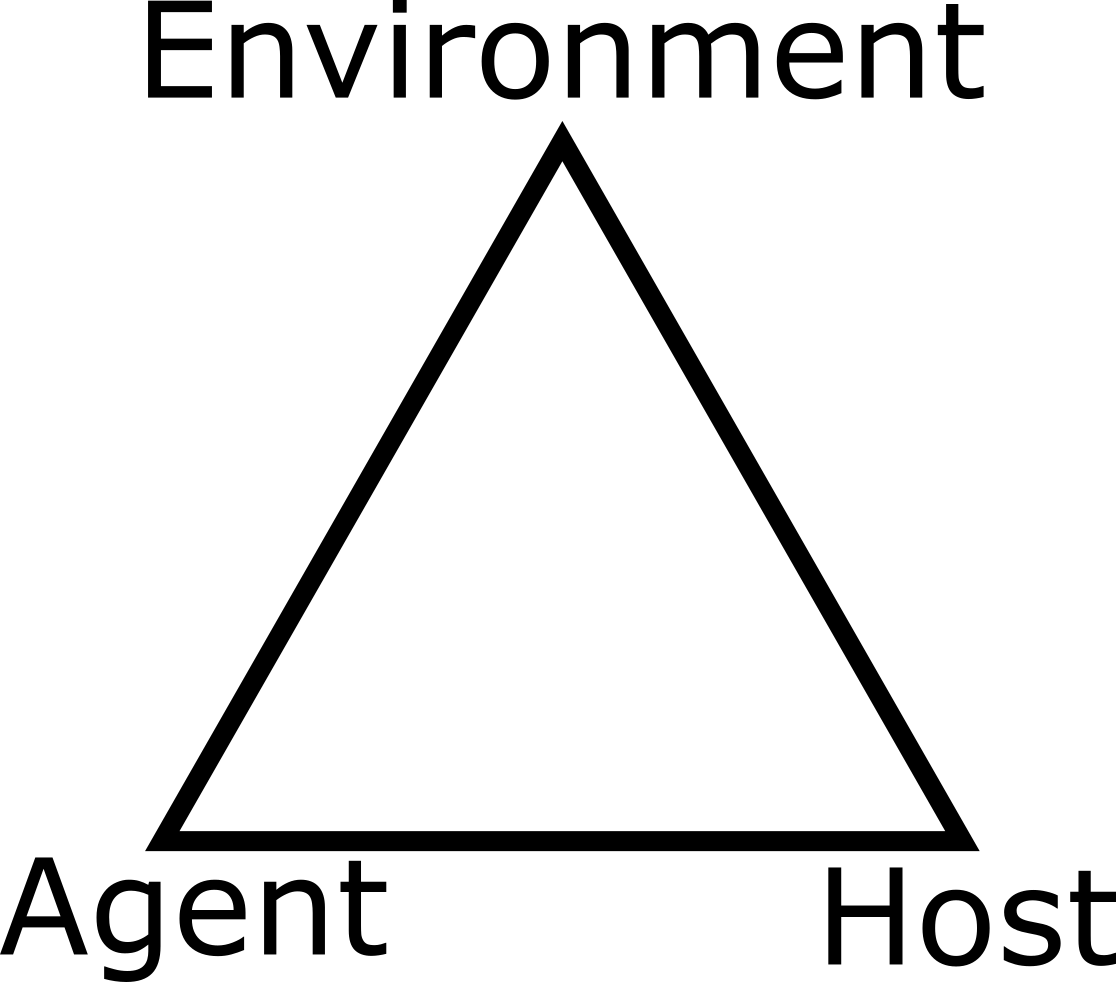
\includegraphics{./images/epi-triangle.png}
\caption{\label{fig:epitriangle}A system perspective - The epidemiological
triangle}
\end{figure}

Similarly, one can think of the basic epidemiological concept of
\emph{person - place - time} as describing a system. The notion of a
system is present in virtually every field of research, ranging from the
hard sciences to social sciences and business.

The scientific approach that has generally been the most successful in
the past was to break down a system into its components and study the
components one at a time. Usually referred to as the
\emph{reductionistic approach}. This approach to understanding the world
is still very powerful and useful.

A complementary approach, which has seen increased use, is to look at
``the whole'' system at once, instead of each component at a time. Using
the whole system approach can provide insights that might not be
obtained by the purely reductionist approach. Looking at the whole
system at once is often referred to as \emph{systems thinking/approach}.

\section{Systems Thinking}\label{systems-thinking}

The term \emph{systems thinking} or \emph{systems approach} or similar
such terminology has become popular in various fields during the last
few decades. It is not a very clearly defined term, but in general, a
\emph{systems} perspective looks at multiple - often many - components
that interact with each other in potentially complicated ways.

For instance, the problem of obesity has many different components that
interact in potentially complex ways to affect a person's weight. Figure
\ref{fig:obesitysystem} illustrates this, see also for instance
\href{https://youtu.be/2vojPksdbtI}{this video}. Complex systems are
everywhere. The approach of studying (most of) the system at once
instead of looking at a single component at a time is the hallmark of
the \emph{systems approach}.

\begin{figure}
\centering
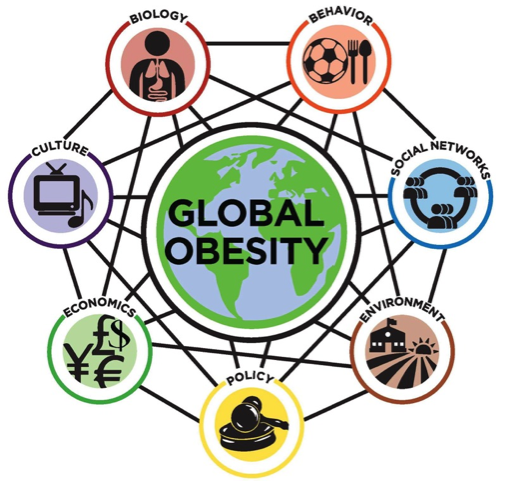
\includegraphics{./images/complexsystem.png}
\caption{\label{fig:obesitysystem}Obesity as a complex system:
\url{http://goo.gl/m2Qq13}}
\end{figure}

\section{Classical and Systems ID Epi
Approaches}\label{classical-and-systems-id-epi-approaches}

While concepts such as the epidemiological triangle acknowledge that
interactions between components are important and determine the behavior
of a system, in practice the standard epidemiological approach, based on
classical study designs such as cohort, case-control and the randomized
trial does not consider system interactions. Indeed, a hallmark
assumption of these study designs is that individuals are independent.
E.g. the chance that someone in a cohort study has the outcome of
interest does not affect the chance of someone else having the outcome.
That works well for non-transmissible diseases, and to some extent for
transmissible/infectious diseases (we'll use the term infectious disease
in the following, mostly meaning diseases that are also transmissible),
as long as there are no interactions (i.e.~contact that could lead to
transmission) between study subjects. Accounting for interactions
between hosts is required to understand important infectious disease
concepts such as population level immunity thresholds, critical
community size, or indirect effects of interventions. This, in turn,
requires a systems approach that explicitly allows for interactions
between hosts.

On the research side, the importance of such interactions has long been
appreciated and is at the core of the infectious disease modeling
paradigm, where one builds and analyzes a system of interacting
components (e.g.~susceptible and infected hosts). Model based system
approaches have a long history in infectious disease epidemiology
(Anderson and May \protect\hyperlink{ref-anderson91}{1991}, Blower and
Bernoulli (\protect\hyperlink{ref-blower04}{2004})). The importance of
computational methods for the study of infectious diseases continues to
increase. In this book, we approach infectious diseases from such a
systems thinking perspective, without delving too deeply into the
mathematical and computational aspects of the topic.

\section{Sytems Thinking and Models}\label{sytems-thinking-and-models}

Models are everywhere in science. Models can be conceptual (e.g.~graphs
or charts), experimental model systems (e.g.~a specific mouse strain in
immunology) or take the form of mathematical/computer models.

Once we take the systems perspective, we have to deal with many
components that interact in potentially complicated ways. Making study
and analysis complicated, especially if we are trying to gain insights
into the causal and mechanistic connections between some quantity
(exposure) and some outcome. When taking a systems approach, it is
therefore often not enough to have a conceptual model alone. While a
conceptual approach often allows some qualitative understanding, it is
somewhat limiting. It is for instance almost impossible to gain a good
\emph{quantitative} understanding how changes in certain conditions and
components of a system lead to changes in outcomes of interest by
relying on conceptual approaches alone. If we want to go beyond
qualitative and move toward a quantitative understanding (i.e.
`increasing the tobacco tax by X\% will reduce smoking-related health
care costs by Y\%'), we need mathematical/computational models. There
are many different types of models one can implement. The following
provides a - very brief - overview of different modeling approaches.

\subsection{Phenomenological (statistical)
Models}\label{phenomenological-statistical-models}

A huge class of models consists of what we usually refer to as
statistical models. In the context of this discussion, I prefer to label
them \emph{phenomenological} models, but that terminology is rarely
used. The idea behind the statistical/phenomenological approach is to
use a mathematical or computational model to study if there are any
patterns between the input (exposure and other variables) and the output
(outcomes of interest).

For instance, a linear regression model investigates if there is a
pattern/correlation between input and output that can be well
approximated by a linear function. More complicated statistical models
exist, some go by the name of \emph{machine learning methods}. All of
these models try to determine if there are patterns between inputs and
outputs of interest in the data.

One feature these statistical/phenomenological models have in common is
that they do not try to describe the mechanisms of interactions within
the system that lead to the observed input-output relations. For
instance, if we find that the relationship between the number of
cigarettes smoked per day and the 5-year risk of lung cancer can be
approximated by a linear function, it does not tell us much about the
mechanisms leading from smoking to lung cancer.

\subsection{Mechanistic Models}\label{mechanistic-models}

Another class of models are mechanistic models, which explicitly -
albeit usually in very simplified form - try to model the mechanisms of
interaction among system components. These models are commonly used for
infectious disease studies. For instance, we might want to know how drug
dose affects pathogen clearance inside an infected patient. We could
collect data on both (such data often needs to come from animal models)
and see if a straight line or another kind of model fits the data.
Alternatively, we could try to build a model that explicitly captures
the mechanism of the drug killing the pathogen, and then see if this
mechanistic model describes the data well. The advantage of these kinds
of models is that they potentially provide better and deeper
understanding of the system. The main disadvantage is that we already
need to know (or at least assume) a good bit about how the components
interact for us to be able to build such a model. If we don't know what
mechanisms might lead to some input impacting some output, we can't
build a mechanistic model.

Both phenomenological (statistical) and mechanistic models are useful
tools with distinct advantages and disadvantages. Deciding which one to
use depends on the question and study system. In this book, we will
focus on mechanistic models, which try to represent an explicit,
simplified description of the system of interest.

\subsection{Dynamical Systems
Thinking/Modeling}\label{dynamical-systems-thinkingmodeling}

The dynamical part adds an explicit time component to the system (and
assumes that we can use equations to describe the dynamics). Consider
this example: We could study how a change in tobacco taxes might lead to
changes in healthcare costs in a given state. Of course, time is present
in this system: First we change the taxes, and then we look at changes
in costs over some time frame. However, when studying this system, one
usually doesn't need to consider an explicitly time-dependent dynamic.
Instead one looks at 2 scenarios: Taxes 1 \& Costs 1 versus Taxes 2 \&
Costs 2. It is usually not necessary to model or simulate the chain of
events leading from tax change to cost change while explicitly
accounting for time.

In contrast, in a dynamical system, the model explicitly changes in
time. We might often want to know how certain changes to the system
(e.g.~interventions) lead to changes in outcomes through a
\emph{dynamical/time-dependent} chain of events. For infectious
diseases, we most often have some underlying dynamics that we need to
take into account (e.g.~an ongoing outbreak) and on top of which we
might want to implement some interventions. Therefore, the dynamical
perspective is often used. Even if a specific disease can be considered
to be `steady' before we implement an intervention (e.g.~a given level
of TB in a country), there is still disease transmission between
individuals happening, which most often makes the dynamical approach
more suitable.

We can illustrate this dynamical perspective by extending the
epidemiological triangle. Figure \ref{fig:dynamictriangle} shows the
components and the interactions of the triangle changing over time.

\begin{figure}
\centering
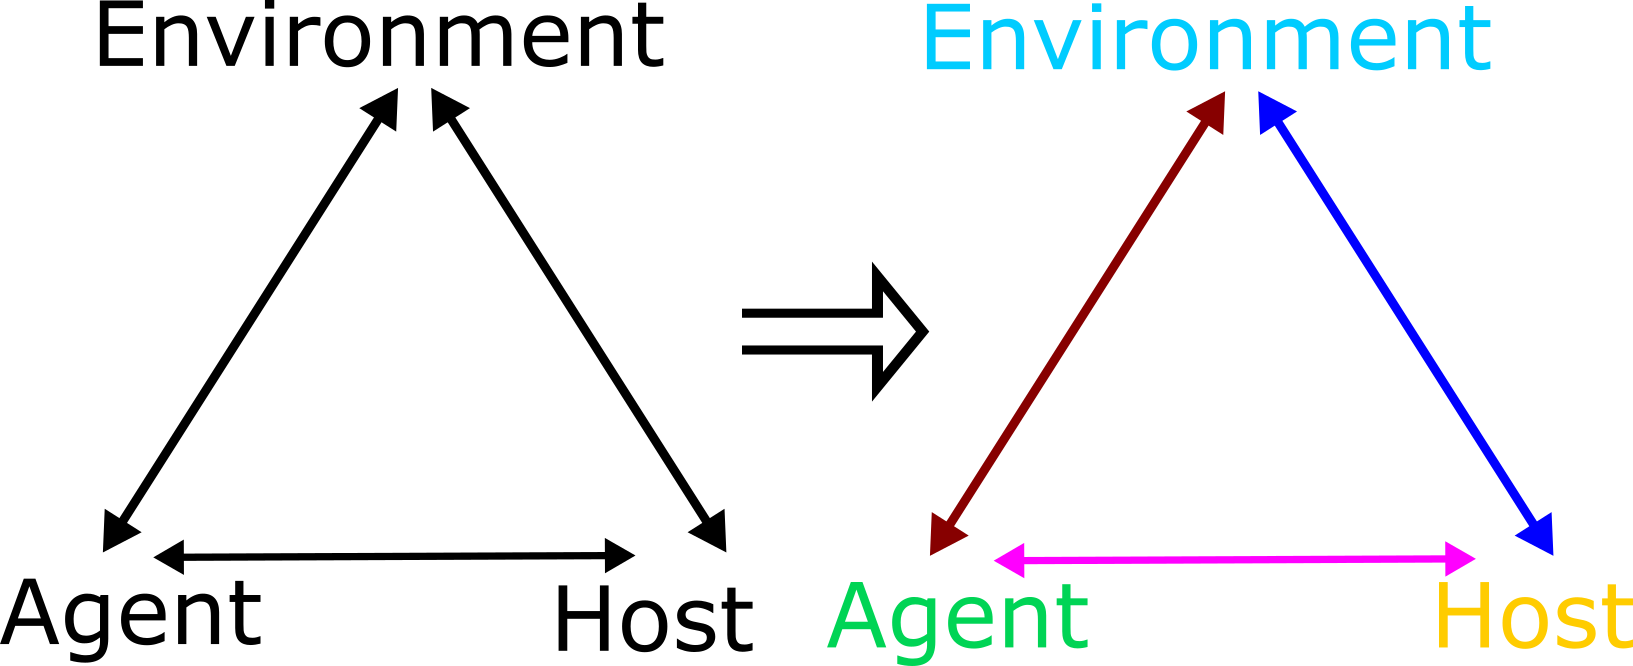
\includegraphics{./images/moving-triangle.png}
\caption{\label{fig:dynamictriangle}Dynamic Epidemiological Triangle.
Interactions between agent, host and environment change explicitly with
time - indicated by the different coloring for each component and
interaction.}
\end{figure}

Mechanistic models are especially well suited to describe dynamical
systems and are therefore the primary choice for the study of complex
dynamical systems.

\subsection{Types of Dynamical, Mechanistic
Models}\label{types-of-dynamical-mechanistic-models}

When building mechanistic, dynamical models based on a systems approach,
there are two main approaches. In one approach, the model is made up of
individual \emph{agents/individuals} and is thus called Agent based or
Individual based model. The agents/individuals - which are often but not
always are humans - interact with each other. Each agent has certain
properties and undergoes certain actions. The interactions of all the
agents lead to potentially interesting and complex dynamics. Schelling's
segregation model (see e.g. \href{https://youtu.be/dFl3Cfw12bo}{this
video} ) is a nice example of such an agent based model. Models and
approaches that consider individuals connected through networks of
contacts are particularly important for infectious diseases, and we'll
briefly discuss those in a later chapter.

Another approach simplifies the system by not tracking every individual
agent, but instead only keeps track of total agents/individuals in
certain states. For instance, for an ecological model, we might track
the total numbers of predators and prey (e.g.~wolves and sheep). The
resulting model is significantly simplified compared to the agent based.
If we had a population of a 100, 1000 or 10,000 wolves or sheep, we
would need to keep track of as many agents. If we only keep track of the
total number of individuals, we only need to track how the numbers in
each \emph{compartment} (here wolves and sheep) change - no matter how
large our population. Those models, which only track total numbers of
individuals, are called \emph{compartmental models}

While these compartmental models are obviously simplifications of the
real system, they often retain enough of the model complexity to allow
us to study the system in detail. Because of this, the majority of
models used in infectious disease epidemiology are still these types of
compartmental models. Both the DSAIDE R package and the example models
shown in this book focus on such compartmental models. For some more
information on compartmental models,
\href{https://en.wikipedia.org/wiki/Compartmental_models_in_epidemiology}{check
out this Wikipedia article}

\section{A Basic Infectious Disease Systems
Model}\label{a-basic-infectious-disease-systems-model}

For infectious disease models, the simplest dynamical systems model
keeps track of the total number of individuals who are susceptible,
infectious and recovered/immune (the so-called SIR model). This model is
a compartmental model, i.e.~we place individuals into distinct
compartments, according to some characteristics. We then only track the
total number of individuals in each of these compartments. In the
simplest model, the only characteristic we track is a person's infection
status according to 3 different stages/compartments:

\begin{itemize}
\tightlist
\item
  \textbf{S} - uninfected and susceptible individuals.
\item
  \textbf{I} - infected and infectious individuals (note that these
  terms are often used interchangeably, but technically we are talking
  about someone who is infected \textbf{and} is infectious, i.e.~can
  infect others).
\item
  \textbf{R} - recovered/removed individuals. Those are individuals that
  do not further participate, either because they are now immune or
  because they died.
\end{itemize}

In addition to specifying the \textbf{compartments} of a model, we need
to specify the \textbf{processes/mechanisms} determining the changes in
each compartment. Broadly speaking, some processes increase the number
of individuals in a given compartment/stage and processes that lead to a
reduction. Those processes are sometimes called inflows and outflows.

For our system, we specify only 2 processes/flows:

\begin{enumerate}
\def\labelenumi{\arabic{enumi}.}
\tightlist
\item
  A susceptible individual (S) can become infected by an infectious
  individual (I) at some rate (for which we use the parameter \emph{b}).
  This leads to the susceptible individual leaving the S compartment and
  entering the I compartment.\\
\item
  An infected individual dies or recovers and enters the
  recovered/removed (R) compartment at some rate. This is described by
  the parameter \emph{g} in our model.
\end{enumerate}

The SIR model is very basic, but it still has the hallmark of a complex
system. Specifically, there is an interaction between components, namely
the \textbf{I} ``component'' interacts with the \textbf{S} component, or
phrased in more ordinary language, infected individuals can interact
with susceptibles and thereby infect them.

For compartmental models (and often other types of models), it is useful
to show a graphical representation of the compartments and processes
included in the model. For compartmental models, such a diagram/figure
is usually called a flow diagram. Such a diagram consists of a box for
each compartment, and arrows pointing in and out of boxes to describe
flows and interactions. For the simple SIR model, the flow diagram is
shown in Figure \ref{fig:basicSIR}.

\begin{figure}
\centering
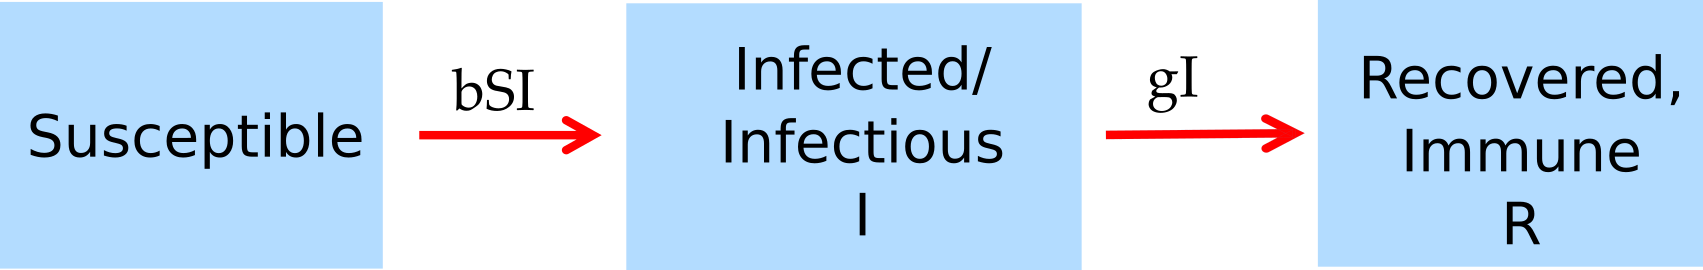
\includegraphics{./images/basicSIRmodelfigure.png}
\caption{\label{fig:basicSIR}Flow diagram for the simple SIR model.}
\end{figure}

\subsubsection{Model Implementation}\label{myadvancedbox}

If one wants to study any model in detail, one needs to implement it
either in the form of a mathematical or a computer model (or both). For
compartmental models, the most common way of implementation is writing
the model as a set of ordinary differential equations and implementing
those in some computer language. This book shows sets of ODE equations
for the several of the discussed models, but a detailed understanding of
these equations is not required to understand the different topics we
discuss. For the model described above, the equations look like this:
\[\dot S = -bSI\] \[\dot I = bSI - gI\] \[\dot R = gI\]

We are using the usual short-hand notation, where a dot over a variable
means its derivative (its change) with respect to time. In all the
models we consider, we always only consider changes with respect to time
(the dynamical aspect of the model).

\section{Some General Comments and
Notes}\label{some-general-comments-and-notes}

In general, the entities that change (that vary) in our system (here the
number of individuals in compartments S, I and R) are called variables
and are each given a compartment/equation. In contrast, the quantities
that are usually assumed fixed for a given system are called parameters.
For the model above, those are the infection rate \emph{b} and the
recovery rate \emph{g}. This is not a fixed rule, though and sometimes,
parameters can be allowed to vary.

When talking about the quantities that are tracked in each compartment,
you will see both the term \emph{host(s)} and \emph{individual(s)} used
interchangeably. While we most often think of human hosts, the hosts can
be any animal (or plants or bacteria infected by phages, etc.).
Sometimes, a compartment might track an entity such as pathogen load in
the environment.

If you want to study a specific ID, you choose parameters such that they
match the specific disease you want to study. We'll return to that idea
throughout this book.

Unfortunately, there are no rules concerning the naming of variables and
parameters. Compartments (e.g.~SIR) tend to be labeled very similarly by
different researchers, while parameter labels are much more variable.
I'm trying to be consistent in this book, though I might mix it up
occasionally. For this book, I decided to stick with letters from the
English alphabet, but you can often find people use Greek letters for
parameters (e.g. \(\beta\) instead of \emph{b} for the transmission
parameter). Always check carefully for a given paper/model what the
definition and meaning of each variable and parameter are.

\section{Summary and Cartoon}\label{summary-and-cartoon}

This chapter provided a brief introduction to the concept of systems
thinking and how modeling is used to study complex systems. We briefly
looked at a simple infectious disease systems model, the famous SIR
model.

\begin{figure}
\centering
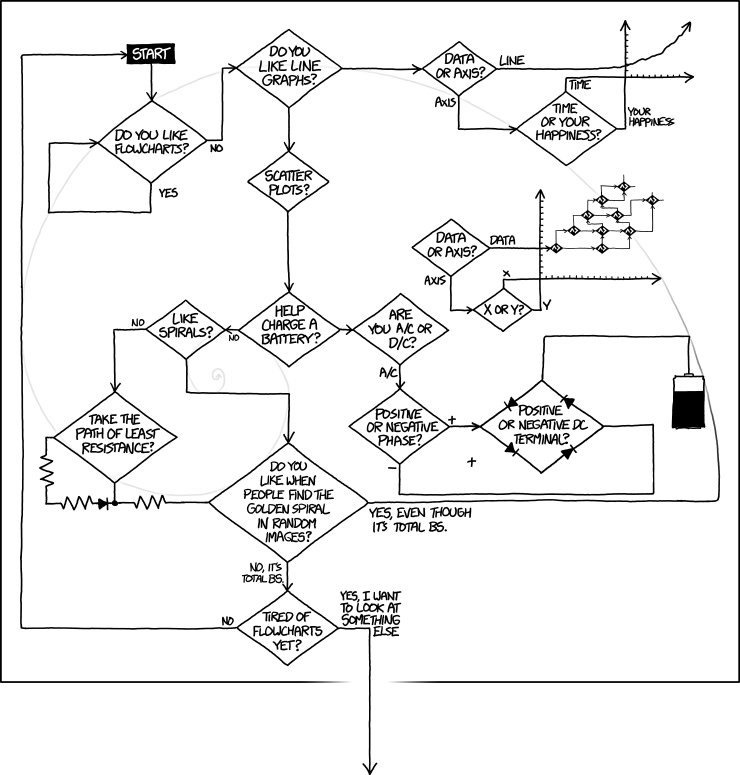
\includegraphics{./images/xkcd-flowcharts.png}
\caption{\label{fig:complexcartoon}Not every diagram helps to understand a
complex system. \href{https://xkcd.com/1488/}{Source: xkcd.com}.}
\end{figure}

\section{Exercises}\label{exercises}

\begin{itemize}
\tightlist
\item
  Work through the tasks for the \emph{ID Dynamics Introduction} DSAIDE
  app.
\item
  Contemplate on your experience with the \emph{ID Dynamics
  Introduction} DSAIDE app. In which way does it capture the `dynamical
  systems' perspective? Did you find any behavior of this - arguably
  still very simple - infectious disease model/system that you would
  consider as being ``complex''? How/why?
\item
  Read the paper ``Systems Science Methods in Public Health: Dynamics,
  Networks, and Agents'' by Luke \& Stamatakis (Luke and Stamatakis
  \protect\hyperlink{ref-luke12}{2012}). Come up with 2 systems that you
  consider complex in the realm of public health or biomedicine (other
  than those mentioned in the paper). Explain what makes them complex.
  Also, come up with 2 systems that you consider not complex and explain
  why you think of them as not complex.
\end{itemize}

\section{Further Resources}\label{further-resources}

\begin{itemize}
\tightlist
\item
  The paper ``Why Model?'' by Joshua Epstein (Epstein
  \protect\hyperlink{ref-epstein08}{2008}) provides a nice, short
  discussion of the purposes of models. Other general introductory
  discussions of systems thinking and model use are (May
  \protect\hyperlink{ref-may04}{2004}; Chubb and Jacobsen
  \protect\hyperlink{ref-chubb10}{2010}; Garnett et al.
  \protect\hyperlink{ref-garnett11}{2011}; Basu and Andrews
  \protect\hyperlink{ref-basu13}{2013}; Gunawardena
  \protect\hyperlink{ref-gunawardena14}{2014}; Homer and Hirsch
  \protect\hyperlink{ref-homer06}{2006}; Peters
  \protect\hyperlink{ref-peters14}{2014}; Sterman
  \protect\hyperlink{ref-sterman06}{2006}).
\item
  Several introductory papers on infectious disease modeling can be
  found in e.g. (Keeling and Danon
  \protect\hyperlink{ref-keeling09}{2009}; Heesterbeek et al.
  \protect\hyperlink{ref-heesterbeek15}{2015}; Lessler et al.
  \protect\hyperlink{ref-lessler16}{2016}; Metcalf and Lessler
  \protect\hyperlink{ref-metcalf17}{2017}).
\item
  While the dynamical systems approach has been applied to infectious
  diseases for a long time, it is starting to be used more frequently in
  other areas of public health. Some recent references on that topic are
  e.g. (Ness, Koopman, and Roberts \protect\hyperlink{ref-ness07}{2007};
  Sánchez-Romero et al. \protect\hyperlink{ref-sanchez-romero16}{2016}).
\end{itemize}

\section{References}\label{references-1}

\chapter{Characterizing Infectious Disease
States}\label{characterizing-infectious-disease-states}

\section{Overview and Learning
Objectives}\label{overview-and-learning-objectives-1}

In this module, we will discuss ways to characterize individuals with
regard to their ID status. We will consider why some infection states
are important for public health control but less for doctors and the
opposite. We will also discuss how different ID states might or might
not correspond to the compartments in our computer models.

The learning objectives for this chapter are:

\begin{itemize}
\tightlist
\item
  Categorize infectious diseases according to medical characteristics
  such as duration of symptoms, mortality, etc.
\item
  Categorize infectious diseases according to public health
  characteristics such as duration of infectiousness, immunity, etc.
\item
  Understand how ``medical states'' (e.g.~symptoms) and ``public health
  states'' (e.g.~infectiousness) do not always overlap.
\item
  Identify the features of infectious diseases that are most important
  to know for successful intervention planning
\item
  Understand how models change as more details are included
\end{itemize}

\section{Introduction}\label{introduction-1}

We previously introduced a very simple compartmental systems model for
an infectious disease (the SIR model) where individuals were split
according to 3 states: susceptible, infected (and infectious) and
recovered (and immune). While easy and sometimes a good starting point,
the simple SIR is often not detailed enough to capture the important
aspects of many infectious diseases. Here, we discuss some important
considerations with regard to the infection status of individuals that
can affect the behavior of the system and thus need to be included if
one wants to build a model to study this system.

\section{Infection states}\label{infection-states}

It is important to keep in mind that infectiousness and symptoms are not
always overlapping. The former is the most important driver of the
ongoing infection process. The latter is important for surveillance and
medical interventions. We will discuss different clinical/medical and
epidemiological/transmission states in the following.

\subsection{Infection states -
clinical}\label{infection-states---clinical}

From a purely medical perspective, focusing on one patient at a time,
the most important characteristic of a disease is its severity, also
called morbidity. We would like to know what kind of symptoms a disease
produces and how frequently those occur. This is the morbidity profile
of a disease. One can consider mortality the ``ultimate symptom''.
Because of its importance, mortality is often considered separate from
morbidity. Knowing morbidity and mortality of an ID are generally most
important when caring for individual patients. For interventions,
understanding what might help mitigate morbidity and mortality is of
prime interest. Morbidity and mortality are also often necessary for the
acquisition of data. It is difficult to determine infected individuals
that do not show symptoms, those that are symptomatic - and obviously,
those that die - are easier to count and thus get estimates for disease
prevalence and incidence.

\subsection{Infection states -
epidemiological}\label{infection-states---epidemiological}

From the perspective of a public health practitioner, other ID
characteristics besides morbidity and mortality are fundamental. We need
to know when someone is infectious (e.g.~before/without symptoms, or
only when symptomatic), how transmission occurs, if recovered
individuals become immune, if immunity is waning, etc. The difficult
part is that our data often comes from clinical (symptomatic) cases or
deaths. If asymptomatic individuals are infectious, or there is
underreporting, we often don't get the full picture.

Of course, the medical and epidemiological perspectives are not an
`either/or'. Instead, success in combating infectious diseases only
comes when all aspects are considered. Still, it is useful to keep in
mind that certain infection states are more important when considering
how to intervene on the individual patient level versus intervention on
a population level.

\subsubsection{Biased Surveillance - an example}\label{myexamplebox}

During the early days of the 2009 H1N1 influenza pandemic, the numbers
on cases and deaths suggested that this strain of influenza might have a
higher than normal case fatality ratio (the often used term case
fatality rate is a bad label as this is not a rate). Once more and
better data became available. It was realized that many infections
initially did not get reported, and adjusting for those it became clear
that the ratio of deaths to infected was thankfully not much different
from seasonal influenza.

\section{Other important infectious disease
stages}\label{other-important-infectious-disease-stages}

In addition to the infection stage, other states of the host might need
to be considered carefully. For instance, while in the classic SIR model
the recovered individuals are assumed to be immune to re-infection - and
thus don't further influence the systems dynamics, there are IDs which
either do not induce immunity (e.g.~many sexually transmitted diseases)
or only lead to short-term immunity (e.g.~norovirus or influenza). This
can often be represented in a model by adjusting the flows, e.g.~if
recovered individuals initially have some immunity and then lose them,
flow from the recovered to the susceptible class can be implemented.

\subsection{Models with more details}\label{models-with-more-details}

To study the dynamics of an infectious disease in more detail than is
provided by the simple SIR model, we can consider models that allow for
additional states. Figure \ref{fig:complicatedmodel} shows a model with
additional compartments. Equations for this model are not shown here,
but a model similar to this one, together with the equations, can be
found in the corresponding DSAIDE app referred to below.

\begin{figure}
\centering
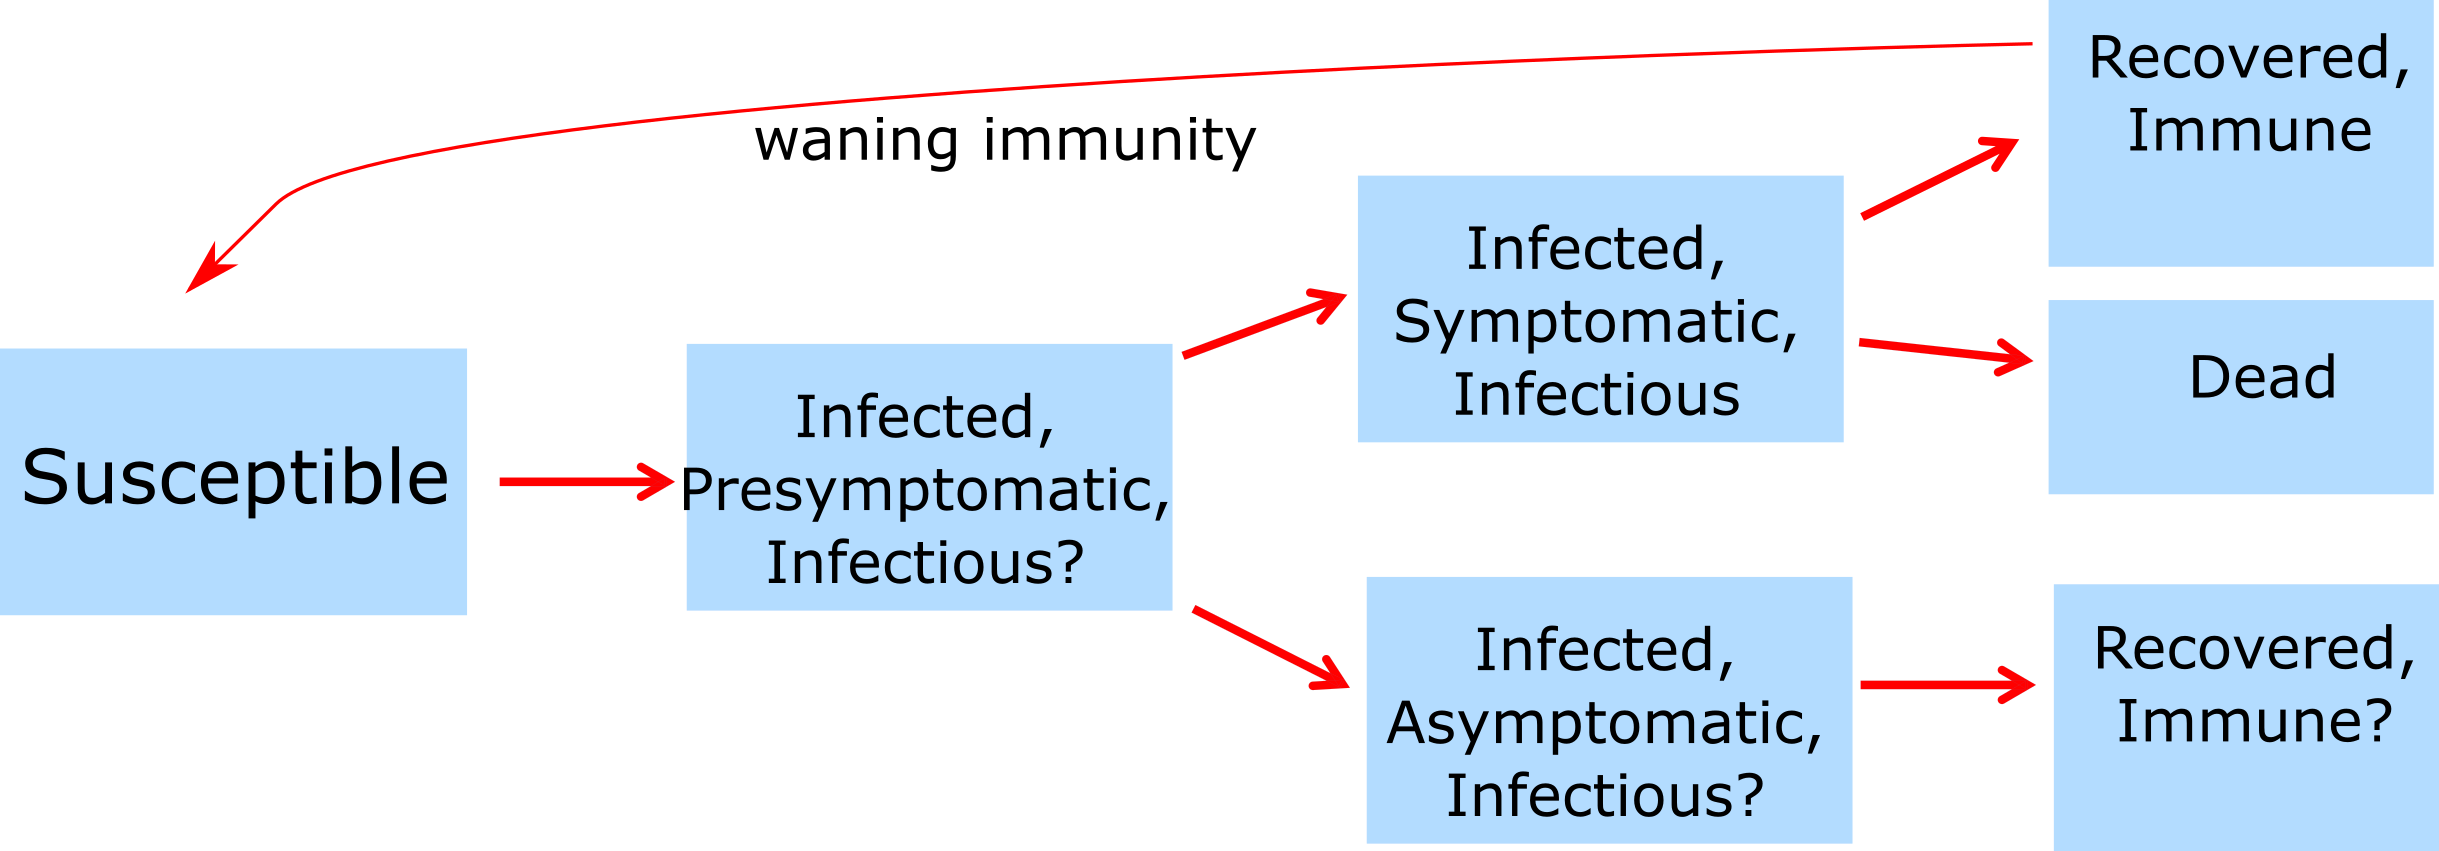
\includegraphics{./images/ComplicatedModel.png}
\caption{\label{fig:complicatedmodel}Example of a model with more
compartments.}
\end{figure}

\section{How complex should our model
be?}\label{how-complex-should-our-model-be}

Individuals can be classified as non-infectious or infectious. The
latter could be divided further, e.g.~into low and high infectiousness.
Infectiousness is the primary driver of the dynamics. Clinical states
that are often tracked are asymptomatic, symptomatic and dead.
Sometimes, individuals are asymptomatic before they become symptomatic.
This is usually labeled pre-symptomatic. Individuals in any of those
states can be infectious or not. Depending on the ID, some of those
states are more important than others. For instance for HIV, individuals
are infectious during the long asymptomatic period, while asymptomatic
individuals infected with TB are not infectious. A model describing a
specific system needs to be tailored to the ID under study.

The question then becomes: What details should we include and which ones
should we omit? We can - and do not want to - include every detail of a
complex system, i.e.~all components and interactions. We need to decide
which parts are important and need to be in the model, and which ones we
can ignore. A simple and somewhat silly example: We never include the
hair color of individuals in any infectious disease models (at least
I've never seen such a model), since we assume that this characteristic
is not important for the ID dynamics. The choice to include or exclude
other features is less obvious in other cases. For instance, for an HIV
model, we likely need gender, while a SARS model might ignore this
characteristic.

In general, we need to decide for a specific ID, scenario, and question
which details to include in our model and which ones to ignore. In
general, the primary interactions between components of the system are
needed. Thus, if we wanted to model the transmission dynamics of Ebola,
we might need to include deceased infected individuals into the model,
since they are known to contribute to transmission. In contrast, if we
want to study how some control strategies for SARS might reduce the
total number of \emph{infected} but we don't care about the impact on
total deaths (unlikely, but let's just pretend). In this case, we would
not need a dead compartment in our model, since those dead don't further
interact with anyone else in the system. However, if we want to keep
track of deaths and how they are impacted by our intervention (likely),
we do need to track them - even though dead people are not known to
transmit SARS.

We will see many different types of models as we go through the course.
In general, the models will include the feature we are focusing on while
excluding others. For instance, we might include human and mosquitos for
vector-borne IDs but ignore things like asymptomatic or pre-symptomatic
states. This is mainly done to keep models simple and focus on one
feature at a time. Models that address ``real'' questions often -- but
not always -- include a fair number of details.

To build models that are suitable to study a particular system, model
builders need to be experts on the system they want to study and/or
collaborate with subject matter experts.

Building a good model needs to follow the
\href{https://en.wikipedia.org/wiki/Goldilocks_principle}{Goldilocks
Principle}: If a model is too small/simple, it likely doesn't
approximate the real system very well. If the model is too big and
complicated, it 's hard to build, hard to analyze, prone to mistakes,
and might not lead to much insight (i.e.~the model is a big black box).
The goal is to get the model \emph{just right} regarding size and
complexity. Unfortunately, no recipe or formula exists specifying how to
build a \emph{just right} model. Being able to build models that are
appropriate/suitable for a given ID and question distinguishes good
modelers/scientists from less good ones.

Also, the model building and analysis process is often iterative. After
a model has been built and studied, it might become clear -- e.g.~by
comparing the model with data -- that important components or
interactions have been ignored or not been included correctly. This
leads to model modification and refinement. This back and forth between
model and data/the real world can happen over multiple iterations.

\section{Summary and Cartoon}\label{summary-and-cartoon-1}

This chapter discussed ways to characterize an individual host's state
with regard to an infection. We discussed the differences between
medical and public health perspectives and how ID states can be mapped
to models. We also briefly discussed how one should build models that
provide the right amount of complexity.

\begin{figure}
\centering
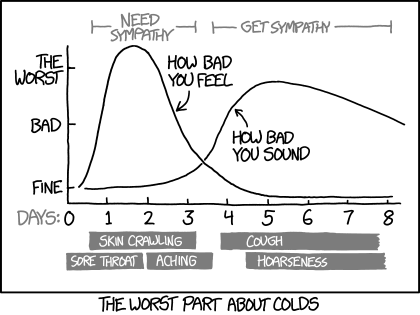
\includegraphics{./images/xkcd-course-of-colds.png}
\caption{\label{fig:coldcourse}Yet another perspective on ID infection
states. \href{https://xkcd.com/1612/}{Source: xkcd.com}.}
\end{figure}

\section{Exercises}\label{exercises-1}

\begin{itemize}
\tightlist
\item
  The \emph{Characteristics of ID} app in the DSAIDE package provides
  hands-on computer exercises for this chapter.
\item
  Suggest a real ID that might be approximately described by the
  \emph{Characteristics of ID} DSAIDE app. Approximately what values for
  the different parameters would be appropriate to describe the ID you
  have in mind? See what you can find for the different parameters of
  the ID you chose in the literature.
\item
  Read the paper ``Modelling an outbreak of an emerging pathogen'' by
  Kajita et al (Kajita et al. \protect\hyperlink{ref-kajita07}{2007}).
  The paper lists 8 assumptions that went into constructing the model.
  Is there any assumption that you might have made differently, and why?
  Are there other assumptions the authors make when building the model
  that are not included in their list of assumptions? If your next step
  would be to further increase model realism, what would you do,
  i.e.~what feature(s) would you include that are currently not in the
  model?
\end{itemize}

\section{Further Resources}\label{further-resources-1}

\begin{itemize}
\tightlist
\item
  The following papers provide some additional information on the ideas
  discussed in this chapter: (Fine \protect\hyperlink{ref-fine03}{2003};
  Milwid et al. \protect\hyperlink{ref-milwid16}{2016}).
\item
  A good example showing how different assumptions about ID states can
  lead to different conclusions, and how models can be used to
  discriminate between alternate hypotheses can be found in (King et al.
  \protect\hyperlink{ref-king08}{2008}).
\end{itemize}

\section{References}\label{references-2}

\chapter{Patterns of Infectious Disease
Dynamics}\label{patterns-of-infectious-disease-dynamics}

\section{Overview and Learning
Objectives}\label{overview-and-learning-objectives-2}

In this module, we will discuss different patterns of ID dynamics, such
as single outbreaks, recurrent cycles, and steady endemic states.

The learning objectives for this chapter are:

\begin{itemize}
\tightlist
\item
  Understand the concept of resource replenishment
\item
  Know the different mechanisms that can lead to ID cycles
\item
  Understand the concept of endemic state
\item
  Understand what leads to different ID patterns
\item
  Understand the difference between intrinsic and extrinsic drivers of
  ID cycles
\end{itemize}

\section{Introduction}\label{introduction-2}

Some IDs produce sporadic outbreaks and then disappear for years. Ebola
is a prominent example. We will discuss in a future module how to figure
out what leads to the (local) extinction of an ID.

Many other IDs show oscillatory behavior, i.e.~we get repeated outbreaks
every so often, with some time of no or little disease in between. For
some ID, the outbreaks are seasonal/annual, for other ID, the cycles are
multi-year.

\begin{figure}
\centering
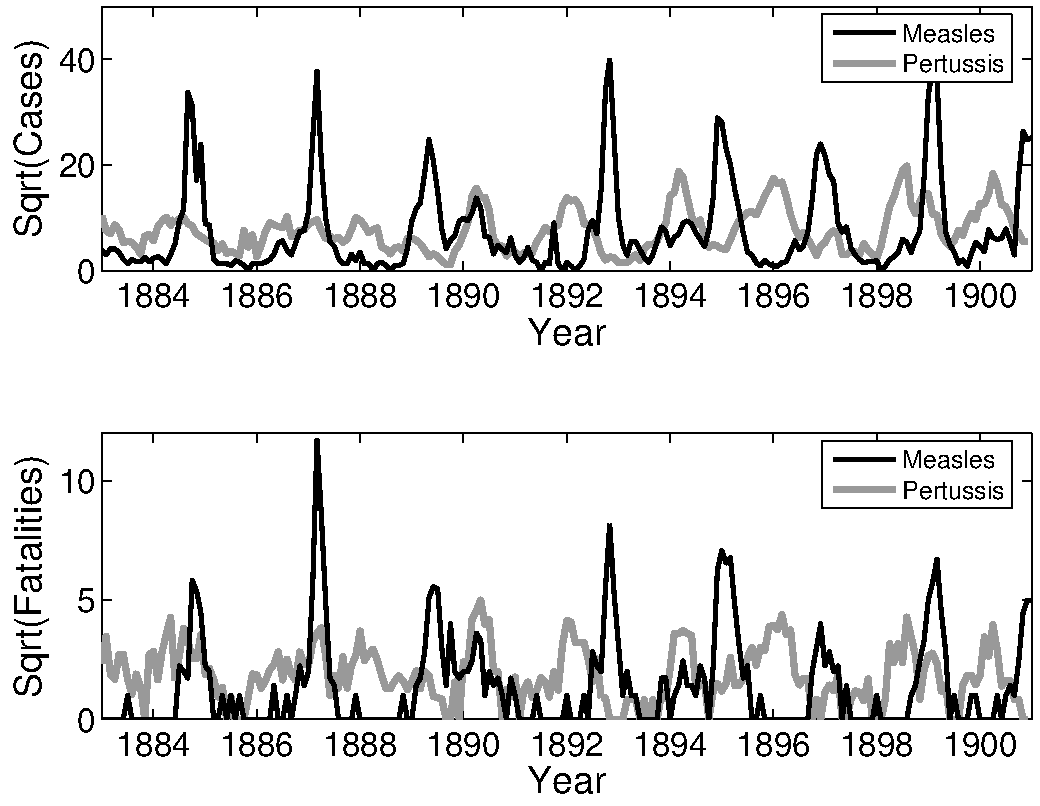
\includegraphics{./images/IDcycles.pdf}
\caption{\label{fig:IDcycles}Examples of ID cycles. From (Keeling and Rohani
\protect\hyperlink{ref-keeling08}{2008}).}
\end{figure}

Why are some ID seasonal, some not? What mechanisms lead to seasonal or
multi-year oscillations? What determines the timing of outbreaks?

Other IDs seem to have ``settled down'' and occur more or less at a
steady level, with only minor fluctuations. TB and HIV in some parts of
the world, as well as certain STD and chronic viral infections of for
instance the herpes virus family, seem to have such a dynamic.

The following discusses the factors affecting these different ID
dynamics patterns.

\section{Resource Replenishment}\label{resource-replenishment}

So far, we mainly looked at scenarios where some ID caused a single
outbreak. As we saw, outbreaks wane because eventually there are not
enough susceptible individuals around to sustain ongoing transmission.
This is a very general ecological principle: Without replenishment of
resources, some consumer of such resources will eventually die out. We
see that in predators eating prey, forest fires ``eating'' trees, and
pathogens ``eating'' their hosts. If the resources are not replenished
quickly enough, the consumer of these resources will go extinct. To
sustain the continued presence of the consumer/predator, resources need
to be replaced.

For our scenario, the resource consumer is the ID, and the resources are
the hosts, usually humans. Replenishment of susceptible hosts can happen
through different mechanisms. Most common is the birth of new,
susceptible individuals, and loss of immunity. Migration, if strong, can
be another way susceptible hosts can be replenished. Similarly,
individuals that become newly sexually active correspond to the birth of
new susceptibles for sexually transmitted infections.

If the replenishment of new susceptibles is rapid, an ID might be able
to maintain itself in a population and never go extinct. (Extinction
will be discussed in more detail later.)

\section{A Model with Resource
Replenishment}\label{a-model-with-resource-replenishment}

A version of the SIR model that includes resource replenishment through
natural births or waning immunity is shown in figure
\ref{fig:birthdeathdmodel}.

\begin{figure}
\centering
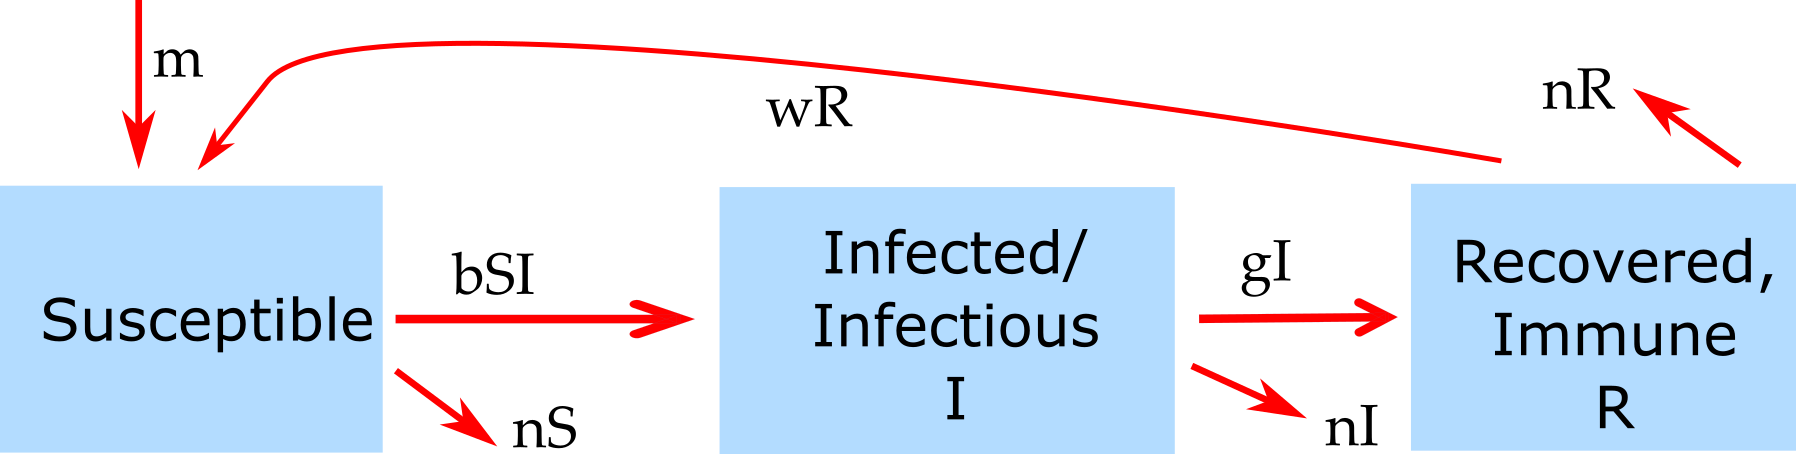
\includegraphics{./images/R0modelfigure.png}
\caption{\label{fig:birthdeathdmodel}Example of an SIR model with births,
deaths and waning immunity.}
\end{figure}

The new features of this model compared to the basic SIR model
introduced earlier are births (of susceptibles) at some rate \emph{m},
natural death at some rate \emph{n}, and the possibility that recovered
lose their immunity and return to the susceptible class at rate
\emph{w}. This new model allows for oscillations/cycles and steady
states, as explained next.

\subsubsection{Mathematical Equations for the Model with Resource
replenishment}\label{myadvancedbox}

The ordinary differential equations corresponding to the compartmental
model shown in figure \ref{fig:birthdeathdmodel} are given by

\[\dot S = m - b I S + wR - n S \] \[\dot I = b IS - gI - n I \]
\[\dot R =  gI - wR - n R\]

\section{Intrinisic Cycles}\label{intrinisic-cycles}

The interaction between susceptible and infectious hosts can lead to a
dynamical pattern that can/does produce oscillations. Specifically, the
dynamics of resource consumption (depletion of susceptible hosts),
waning ID incidence due to reduced availability of hosts, and subsequent
replenishment of susceptibles can lead to cycles. Since these cycles are
not driven by anything ``from the outside'' and arise purely due to the
complex interplay between host resources and ID, there are sometimes
called intrinsic cycles/oscillations. The timing of these cycles (the
period of the oscillations) is determined by characteristics of the ID
and scenario. For instance, the duration of the infectious period and
the transmissibility of the host influence the timing of outbreaks. In
ecology, such cycles are well studied in the context of so-called
predator-prey systems. For our infectious disease models, the ``prey''
are the susceptibles and the ``predators'' are the infected individuals.

\section{Intrinisic Cycles and
models}\label{intrinisic-cycles-and-models}

One can sometimes compute the time between outbreaks. For the simple
compartmental SIR model, an approximate equation for the period close to
the endemic state is
\[T \approx 2 \pi \sqrt{\left( \frac{LD}{R_0 - 1} \right)}\]

Here, \emph{L} is the average lifespan of a host, \emph{D} is the
average duration of infectiousness, and \emph{R\textsubscript{0}} is the
basic reproductive number - a quantity we will discuss shortly. For more
details on this equations, see e.g. (Keeling and Rohani
\protect\hyperlink{ref-keeling08}{2008}).

For more complicated models and real-world scenarios where the simple
SIR model is not a good approximation, the equation just provided does
not apply anymore. It might not even be possible to write down any
equation. One can then instead run a computer simulation of the model
and determine the length of the cycles from the time-series returned by
the computer. The main point still holds, independent of the ability to
write down an equation for the cycle length, namely that there is a
relation between intrinsic characteristics of the system, such as
duration of infectious period (\emph{D}) and transmissibility of the
disease (\emph{R\textsubscript{0}}), and the period of the oscillations.
In cases where we cannot derive a mathematical equation, we can try to
figure out the relation between cycle duration and some parameter of
interest. This can be achieved by repeatedly altering the parameter
(e.g.~the duration of the infectious period, \emph{D}), and recording
the cycle period, \emph{T}, reported by the model simulation for various
values of the parameter. By plotting a figure showing \emph{D} on the
x-axis and \emph{T} on the y-axis, we obtain a relation between these
quantities.

\section{External Drivers of Cycles}\label{external-drivers-of-cycles}

Another mechanism that can lead to oscillations in the dynamics of ID
can come from ``external'' drivers. Of course, these processes are still
part of the whole system, but not as directly as the dynamics and
interaction of the hosts. In that sense, we consider it an external
process.

Weather is one of the most important external factors. Many IDs are
influenced by the weather. For instance influenza virus survives better
when the vapor pressure is low, which in temperate regions is usually
the case in winter (Lipsitch and Viboud
\protect\hyperlink{ref-lipsitch09}{2009}, Shaman et al.
(\protect\hyperlink{ref-shaman10}{2010})).

Other types of seasonality are related to human activity and behavior.
For instance, many childhood diseases increase in incidence when a new
school year starts.

For some ID, weather and behavior interact. Many water-borne diseases in
the U.S. see an uptick in summer. This is due to behavior changes in the
host: More people swim in outdoor water in the summer.

Often, more than one mechanism occurs and influences the ID dynamics. As
such, it is often not possible to isolate a single factor as the main
important one. It often depends on the particular setting.

\section{Notes on Cycles}\label{notes-on-cycles}

In the type of models, we have looked at so far; sustained oscillations
need something like seasonality. Without it, the cycles die out, and the
disease reaches a steady, endemic state. For more complex models or
models that include stochastic dynamics (something we'll discuss later),
cycles can be maintained even in the absence of external drivers.

\section{Steady states}\label{steady-states}

In addition to single outbreaks or recurrent cycles, ID often also reach
a state where the incidence/prevalence in a population is roughly
constant. This is usually referred to as an endemic state. Examples of
that are e.g.~helminth infections in many African countries (in the
absence of control efforts) or certain sexually transmitted diseases in
developed countries.

Note that while at steady state, the total number of ID cases does not
change, there is usually a constant turnover. Some individuals get
infected, while others recover or die. It just happens that these
processes balance each other, making the total numbers roughly constant.

If we have a mathematical or computer model of our system, there are two
ways to determine steady states. One is mathematical, and the other is
through simulating the system. The former approach is more elegant and
powerful but only works if we have a relatively small model. It is
illustrated in the box below. Often, the model is too complicated to
obtain useful equations for the steady state values of the model
variables. Fortunately, we can always determine them numerically. We
simply start our computer simulation model with some values and run it
long enough until it has settled down (we need to make sure it does have
a steady state). We can then record the steady state values. We can do
this for different model parameter values (e.g.~changes in birth rate or
changes of rate of infection). In the end, we can plot a figure showing
how the steady state values change with some model parameter. This
approach is obviously much slower than using the mathematical equations.
However, often it is the only feasible approach.

Note that there are technically steady states that exist but won't show
up in the simulation since they are unstable. Since any unstable steady
state also rarely exists in nature (other than the disease free state,
with a population remaining in that state until a new pathogen arrives),
those steady states tend to be not that important in practice.

\subsubsection{Steady States and Models}\label{myadvancedbox}

When an ID reaches a steady state, a model based on ordinary
differential equations, such as the model shown above, simplifies. At
steady state, there are -- by definition -- no changes in the total
number of individuals in each compartment. Therefore the left side of
the equations are zero, i.e. \(\dot S = \dot I = \dot R =0\). This
changes the differential equations into a set of algebraic equations.
For a fairly small set of equations (usually \textless{} 5), one can
obtain equations for the compartments (\emph{S}, \emph{I}, and \emph{R}
in this case) at steady state that are a function of the model
parameters. While it is often theoretically possible to solve models
with more compartments/equations, the resulting expressions are usually
so big and unwieldy to not provide much useful insight.

The hard method of solving this set of equations is with pen and paper.
Nowadays, there is software that can do it for you. The two most
important packages for such tasks are
\href{http://www.maplesoft.com/}{Maple} and
\href{https://www.wolfram.com/mathematica/}{Mathematica}. Both are
commercial products, fairly powerful and quite expensive. If you only
need a program for occasionally solving such equations, free
alternatives are available. I usually use
\href{http://maxima.sourceforge.net/}{Maxima}.
\href{http://en.wikipedia.org/wiki/Comparison_of_computer_algebra_systems}{Other
packages exist}. Note that \texttt{R} is not suitable for solving
symbolic equations. Using Maxima to solve the equations above (without
immune recovery, i.e. \emph{w=0}, to make the results simpler) gives:

\begin{figure}
\centering
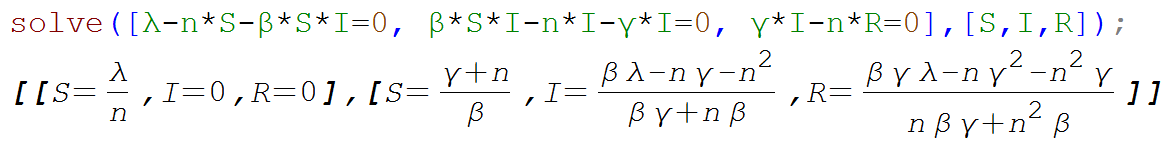
\includegraphics{./images/SSmaxima.png}
\caption{\label{fig:SSmaxima}Maxima code for solving the SIR model steady
state equations.}
\end{figure}

The same results are of course obtained when solving the equations by
hand. The first steady state returned by maxima is the one in the
absence of an ID, with only susceptibles around. Usually, we are
interested in the second steady state, the endemic equilibrium at which
disease prevalence is at a fixed level. We thus find the values for the
number of susceptible, infected and recovered at steady state as a
function of the model parameters.

Having the equations for the steady state allows us to gain insight into
the system behavior rapidly. For instance we can see that for an endemic
steady state to be possible (i.e.~for \emph{I} \textgreater{} 0 at
steady state), we need \(b m > n (n+ g)\). We can make intuitive sense
out of this expression: The combination of pathogen transmission
capacity (\emph{b}) and birth rate \emph{m}, which support ID
persistence, needs to be stronger than the effects of general host death
\emph{n} and host recovery \emph{g}. We will later see that this relates
to the concept of reproductive number.

\section{Detecting cycles or other
patterns}\label{detecting-cycles-or-other-patterns}

It is often hard to determine if there is a specific repeating pattern,
such as oscillations/cycles for a given ID. Consider for instance Figure
\ref{fig:gonorrheapattern}
(\href{http://www.cdc.gov/STD/stats06/images/trends-img-2.gif}{Source
CDC}). One can see that Gonorrhea incidence was fairly stable between
1950-1965 and again 1995-2005, with ups and downs in between. The
changes are not rapid enough to be due to seasonal/annual drivers. If we
had more data and the same up-down pattern repeated, we could speculate
that this might be due to some intrinsic oscillatory dynamics of the
disease. In this case, the most likely explanation for the observed
patterns lies outside the disease dynamics itself. Increased detection
and treatment likely led to a decline in the 40s, changing sexual
behavior lead to an increase starting in the 60s, and strong safe-sex
campaigns, combined with the threat of HIV, resulted in a decrease
starting in the 80s. However, this is somewhat speculative. It might
well be that other factors, (e.g.~changes in surveillance intensity)
could explain the pattern. A careful analysis (which I have not done)
would be needed before one can be more confident as to what might lead
to the observed pattern.

\begin{figure}
\centering
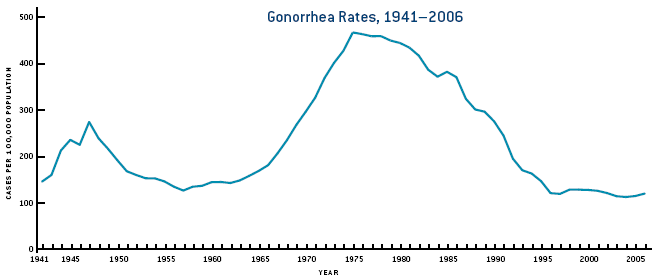
\includegraphics{./images/gonorrhea.png}
\caption{\label{fig:gonorrheapattern}Gonorrhea cases in the US.}
\end{figure}

\section{ID Dynamics in Changing
Populations}\label{id-dynamics-in-changing-populations}

The idea of resource replenishment described above assumes in its
simplest forms that in the absence of the ID, the host population is in
steady state. That is, the number of births and deaths balance each
other, and the population size, therefore, stays constant. We then
investigate ID dynamics on top of such a constant population (which then
might not be constant anymore if the disease leads to many deaths).

One can go a step further and consider an underlying population that
changes in size due to underlying growth or decline of the population.
We can then study the dynamics of an ID on top of an already dynamically
changing population. While this is not much more complicated to do with
computer models, it is harder to understand what exactly is going on in
the system. For instance, consider an ID with high mortality in a
growing population. If we just looked at the population size, it could
be that it remains constant, due to the two processes of natural
population growth and disease induced mortality balancing each other.
We, therefore, need to study how the different processes affect ID
dynamics carefully.

\section{Summary and Cartoon}\label{summary-and-cartoon-2}

This module provided a discussion of the various general patterns we
observe in the dynamics of ID. Those are individual outbreaks, cycles of
repeated outbreaks, and steady endemic states.

\begin{figure}
\centering

\includegraphics{./images/phd_sciencenewscycle.png}
\caption{\label{fig:sciencenewscycle}Here is a different kind of cycle that
(ID) scientists sometimes encounter.
\href{http://www.phdcomics.com/comics/archive.php?comicid=1174}{Source:
phdcomics.com}.}
\end{figure}

\section{Exercises}\label{exercises-2}

\begin{itemize}
\tightlist
\item
  The \emph{Patterns of ID} app in the DSAIDE package provides hands-on
  computer exercises for this chapter.
\item
  Find a scientific article/paper that investigates the
  incidence/prevalence pattern of some ID. Summarize the article.
  Discuss why one sees the observed pattern (and not one of the others).
  Speculate what kind of change to the ID/system could change the
  observed pattern (even if that change is not biologically realistic).
\item
  Read the article ``Dynamical resonance can account for seasonality of
  influenza epidemics'' by Dushoff et al (Dushoff et al.
  \protect\hyperlink{ref-dushoff04}{2004}). They suggest an interesting
  explanation for the seasonal variation in influenza cases. Look at the
  literature to see if since that paper came out, there has been any
  further progress on that question. Discuss recent advances that might
  support or refute the idea suggested by Dushoff et al.
\end{itemize}

\section{Further Resources}\label{further-resources-2}

\begin{itemize}
\tightlist
\item
  The following references provide some more information on and
  discussion of seasonality in IDs: (Altizer et al.
  \protect\hyperlink{ref-altizer06}{2006}; Dowell
  \protect\hyperlink{ref-dowell01}{2001}; Grassly and Fraser
  \protect\hyperlink{ref-grassly06}{2006}; Stone, Olinky, and Huppert
  \protect\hyperlink{ref-stone07}{2007}).
\item
  Seasonality for influenza has been heavily studied, some references
  are (Dushoff et al. \protect\hyperlink{ref-dushoff04}{2004}; Lofgren
  et al. \protect\hyperlink{ref-lofgren07}{2007}; Baumgartner et al.
  \protect\hyperlink{ref-baumgartner12}{2012}).
\item
  A discussion of cycles in Cholera can be found in (Pascual, Bouma, and
  Dobson \protect\hyperlink{ref-pascual02}{2002}; Emch et al.
  \protect\hyperlink{ref-emch08}{2008}).
\end{itemize}

\section{References}\label{references-3}

\chapter{Reproductive Number}\label{reproductive-number}

\section{Overview and Learning
Objectives}\label{overview-and-learning-objectives-3}

The reproductive number is a fundamental concept in infectious disease
epidemiology. It is so important, it even made its way into (at least)
one mainstream movie (``Contagion''
\protect\hyperlink{ref-contagionmovie}{2011})! It is simple in its
definition and rather useful. The hard part is to correctly estimate the
reproductive number for a given disease and scenario. We will discuss
all these aspects in the following.

The learning objectives for this chapter are:

\begin{itemize}
\tightlist
\item
  Know how the reproductive number is defined
\item
  Kow how to compute the reproductive number from data
\item
  Apply the reproductive number concept to ID control
\end{itemize}

\section{Introduction}\label{introduction-3}

We generally want to prevent infectious diseases from causing outbreaks,
stop already ongoing outbreaks, reduce the number of people getting
infected, or even bolder, try to eradicate a disease. If we were able to
make a vaccine against an infectious disease, it is useful to know what
fraction of the population should be vaccinated to prevent future
outbreaks or even eradicate the disease.

Assume you asked the ``person on the street'' the question: ``If we
wanted to prevent a potential future SARS outbreak, what fraction of the
U.S. population do we need to vaccinate to make a large-scale outbreak
impossible?'' I suspect that most people would likely say that nearly
everyone needs to be vaccinated to prevent outbreaks. A smaller number
of people might realize that we don't need to vaccinate everyone, just
enough people to sufficiently reduce the disease's transmission
potential. To reach the second answer, one needs to have thought about
how infectious diseases `work'.

If you happen to come across an ID public health specialist or ID
modeler, you might get a different answer. Namely, they might provide
you with a quantitative estimate of the fraction of people that need to
get vaccinated. They might, for instance, tell you that we would need to
vaccinate around 70\% of the population. This is, of course, the best
kind of information. How do we figure this out? That's where the
reproductive number concept comes into play.

\section{Reproductive number
definition}\label{reproductive-number-definition}

The concept and definition of the reproductive number are rather
straightforward: The reproductive number (usually abbreviated with R),
is defined as the average number of secondary infectious cases caused by
one infectious individual (before they recover or die or are otherwise
not able to further transmit). The following figure illustrates the
concept.

\begin{figure}
\centering
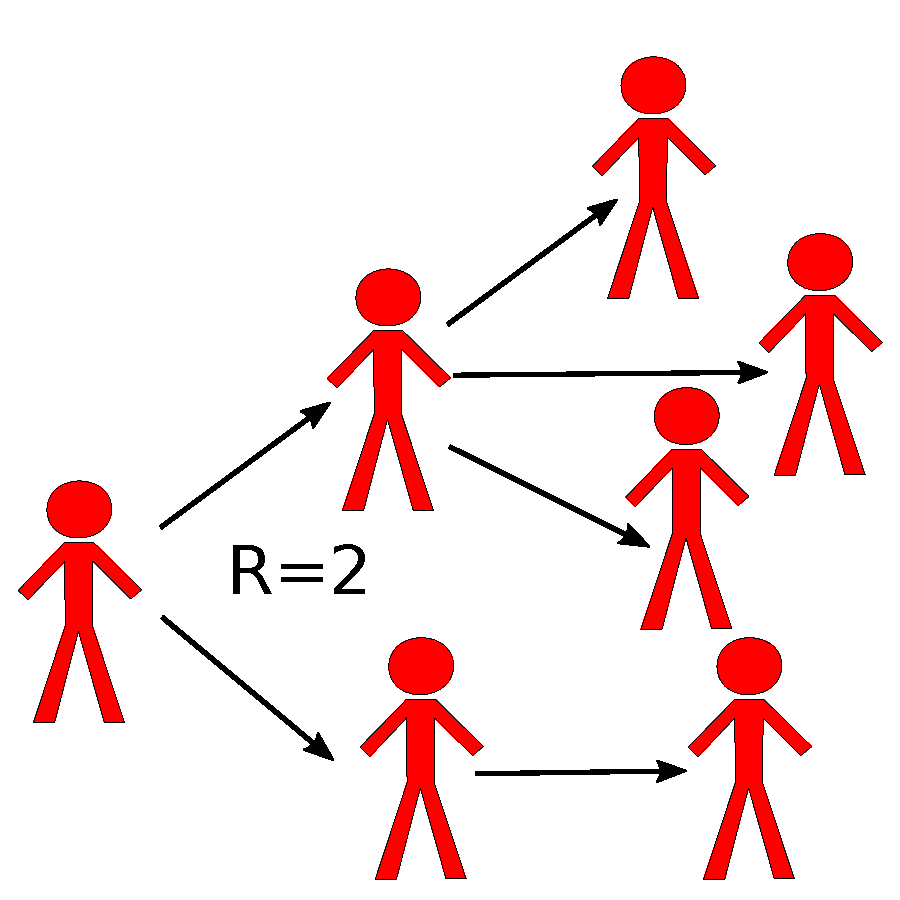
\includegraphics{./images/R0scheme.png}
\caption{Schematic showing the definition of the reproductive number.
Each person `produces' \emph{on average} 2 other infectious individuals.
(Of course, we would usually need to have more data than shown in this
figure to properly estimate R.)}
\end{figure}

From this definition of the reproductive number, it is clear that if the
value is greater than 1, the pathogen keeps spreading to more and more
people and we have a growing outbreak. Conversely, if R is less than 1,
the outbreak will fizzle out. Because of this characteristic, it is
important to know R for a given outbreak, which will then tell us how
stringent the interventions need to be to bring the outbreak under
control. This is more explained in the following sections.

\section{Reproductive number details}\label{reproductive-number-details}

Let's look a bit closer at the definition for R. First, note that it
applies to population \textbf{averages}. A single person might infect
none, a few or many others. R does not capture this detail. It only
describes the average. That's why it is, for instance, possible to have
R=2.5 or other non-integer numbers. Of course, it is not possible for an
individual to infect 2.5 others, but since R describes an average, such
fractional infections are possible. This \textbf{population average}
feature of R is a strength since it makes R relatively easy to
determine. It is also a weakness since often we'd like to know the
distribution in addition to the mean/average - we'll discuss that when
we deal with ideas such as population heterogeneity, core groups, and
super-spreaders in later chapters.

Another point to note is that the definition is about the number of new
\textbf{infectious} hosts produced by one infectious host. For some
diseases, being infected and being infectious are pretty much the same.
E.g. pretty much everyone who is infected with HIV is also - to some
degree - infectious. For other diseases, that is not the case. For
instance, the majority of people who get infected with TB will never
reach a state where they are infectious. To compute R, we do not count
the average number of individuals an infectious person infects, but only
those that later go on to become infectious themselves. The same idea
applies when we talk about diseases that have multiple hosts. R is
defined as the number of infectious hosts `produced' by one infectious
host of the same type. For instance, for vector-borne diseases, R would
be the number of infectious humans `produced' by one infectious human
via the intermediary mosquito/vector stage. While conceptually still
straightforward, measuring and computing R/R\textsubscript{0} in such
multi-host situations can get tricky.

\emph{Note: Here and in other places, I am often sloppy and use the word
``infected'' even if more precisely, I mean ``infectious''. You will
find such sloppy terminology throughout the literature. It is usually
clear from the context if one means an `infected and infectious' person
or just someone who is infected but not infectious (commonly called
``exposed'' or ``latent''). So when you read `infected' here and other
places, assume it means that host is `infectious' as well, unless
otherwise stated.}

\section{Basic reproductive number}\label{basic-reproductive-number}

A special case of the reproductive number is at the beginning of an
outbreak when essentially everyone in the population is susceptible. In
this case, when we assume everyone is susceptible, we define a special
quantity called the \emph{basic} reproductive number, abbreviated as
R\textsubscript{0}. The quantity R\textsubscript{0} is a measurement of
the transmission potential of a disease in a particular setting. It does
by definition not change during an ongoing outbreak. The more general
definition of the reproductive number, R, does change during an
epidemic. We'll discuss that more below.

\section{Notes on the reproductive
number}\label{notes-on-the-reproductive-number}

While I will be mainly using the term reproductive number, there are
alternative names for R. In general, any combination of
reproductive/reproduction and ratio/number is ok terminology. In its
early days, R was called reproductive rate. This is \emph{incorrect}
terminology and should not be used. R is \textbf{not} a rate (there are
no units of inverse time). Why does that matter? See the `R is not a
rate' box for an example.

While we often say ``Infectious disease X has an R\textsubscript{0} of
Y'', this is only an approximation. R and R\textsubscript{0} also depend
on the setting. The potential for transmission for many ID is much
higher in for instance crowded locations (prisons, slums, cruise ships),
or among ``high risk groups'' (e.g.~STD in sex workers). For example
R\textsubscript{0} \textless{} 1 for HIV in the general population but
it is not going away because it has an R\textsubscript{0} \textgreater{}
1 in certain subgroups. When we talk about R, it is, therefore, useful
to specify the scenario/population/setting.

In this reading, and more generally in the literature, you find the use
of R\textsubscript{0}, R or \emph{effective R} (R\textsubscript{eff})
often used (sloppily) in an interchangeable manner. Usually, it's clear
from the context if the symbol refers specifically to \textsubscript{R}0
at the beginning of an outbreak in a susceptible population, or more
generally to R, the average number of secondary infectious cases
produced by one infectious individual in any population.

\subsubsection{Why R Is Not a Rate - Example}\label{myexamplebox}

It is important to understand that R only provides a measure of how
transmissible a pathogen is, R does \textbf{not} provide any information
about the speed at which transmission occurs. This is an important
limitation of R. Consider 2 infections with the similar reproductive
number, say HIV and SARS, which are both estimated to have a
reproductive number of around 3-4. If we let an outbreak `run its
course', we would - based on R - expect to get the same number of
infected individuals. However, the dynamics at which those infections
occur will be quite different. SARS spreads rapidly, i.e.~an infected
person infects 3-4 others within a few weeks. On the other hand, a
person infected with HIV will infect others on a timeframe of years.
These different dynamics have of course important implications on the
control approaches against diseases. Thus, while knowing R is
significant for a given disease, it doesn't tell `the full story'.

\section{Outbreaks and the Change in
R}\label{outbreaks-and-the-change-in-r}

As stated above, at the beginning of an outbreak, a specific disease in
a certain setting will have some value R\textsubscript{0}. As the
outbreak progresses, more and more hosts become infected and - for many
diseases - either die or recover and become immune to further infection.
This leads to a reduction in the reproductive number as the outbreak
progresses. For instance, at the start of the epidemic with everyone
susceptible, R\textsubscript{0}=3. Then once a third of the population
have become infected and immune, an infectious person who would have
infected three others at the beginning of an outbreak now `wastes' one
of their transmissions on an already immune person, and therefore only
infects two others. Similarly, once 2/3 of the population have become
infected and immune, R will have dropped to 1. At this point, the
outbreak does not grow further (recall, we need R\textgreater{}1 for
growth). Instead, the outbreak has reached its peak and now starts to
decline, with R continuing to go down as fewer and fewer susceptibles
remain.

\section{Reproductive Number and Outbreak
Control}\label{reproductive-number-and-outbreak-control}

So how is the reproductive number related to infectious disease
outbreaks? It is intuitively clear that if on average every infectious
person ``produces'' more than one subsequent infectious person, we get a
growing epidemic. In contrast, if every infectious person ``produces''
less than one subsequent infectious person, the pathogen might transmit
a few times, but pretty soon it will disappear. Thus if we can achieve
R\textsubscript{0} \textless{} 1, e.g.~through vaccination, we can
prevent an outbreak from starting. Further, if during an outbreak we can
intervene to get R \textless{} 1, the outbreak is going to fizzle out.
If we wanted to stop any further transmission, we would need to get R
even lower, namely R = 0. Intervention efforts try to achieve an R as
small as possible.

\begin{figure}
\centering
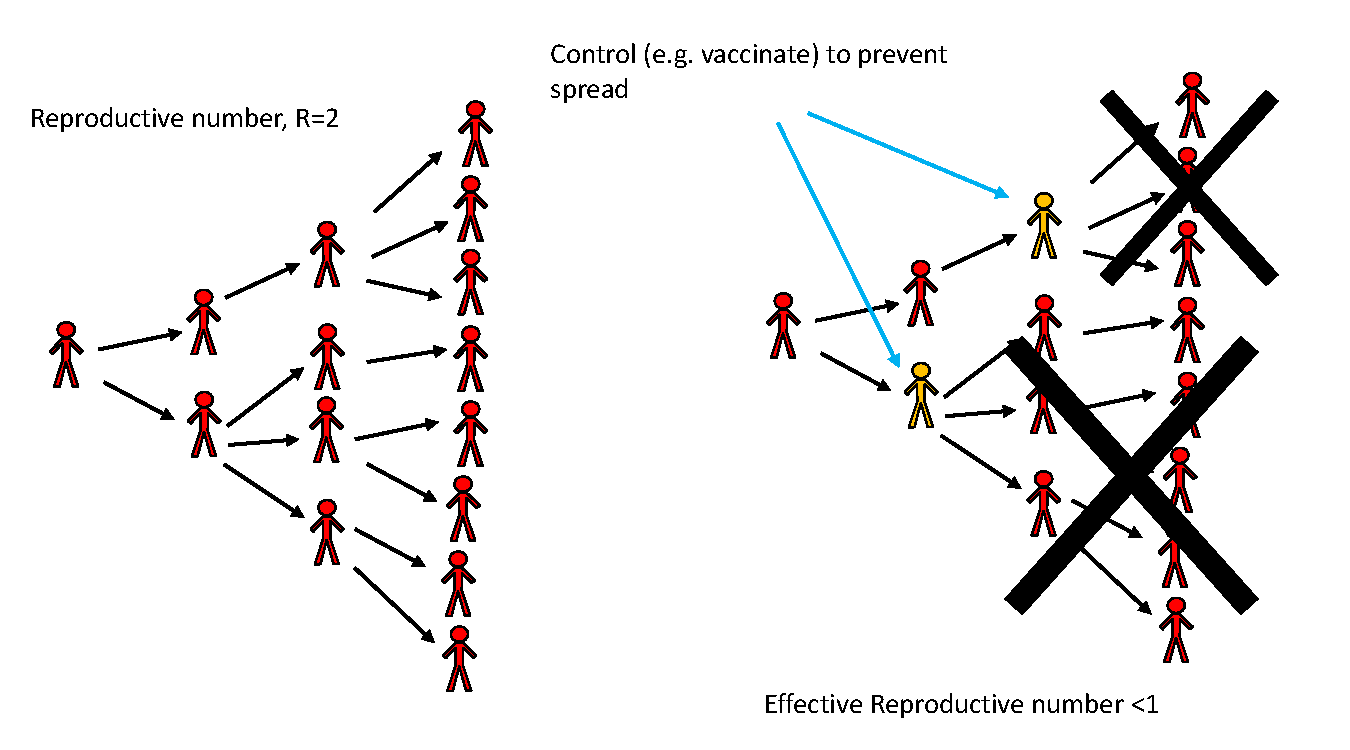
\includegraphics{./images/R0intervention.pdf}
\caption{\label{fig:R0intervention}Impact of an Intervention on
transmission.}
\end{figure}

\subsubsection{R and Outbreak Control - Example}\label{myexamplebox}

During the large Ebola outbreak in West Africa which started in 2013, a
few Ebola patients came to the U.S., and the goal was to have R = 0,
i.e.~no ongoing transmission. That didn't quite happen, a few new
individuals got infected, but R was very close to zero. In contrast, in
West Africa, there was little hope to get R = 0 quickly. Fortunately, R
\textless{} 1 is enough. So we can `tolerate' a few further
transmissions and new cases and still get the outbreak under control
eventually. Of course, in general, we want to get R as close to 0 as
possible, especially for a disease as deadly as Ebola. But to get an
outbreak to fizzle out, we only need R \textless{} 1, not R = 0.

\section{Reproductive Number and ID
Eradication}\label{reproductive-number-and-id-eradication}

If we could achieve R\textsubscript{0} \textless{} 1 globally
everywhere, we could eventually eradicate a disease. The ability to do
that depends on many factors. One important one is the
R\textsubscript{0} value of any ID before we start an eradication
campaign. Intuitively, the higher R\textsubscript{0}, the harder it will
be to get it to \textless{} 1. We'll make that more explicit below.

\section{Connecting Intervention Efforts and
R}\label{connecting-intervention-efforts-and-r}

We just discussed that R \textless{} 1 means no outbreak occurs. Let's
make the relation between response efforts and the reproductive number a
bit more quantitative. As a simple example, consider an infectious
disease with R\textsubscript{0}=2. That means on average every infected
person infects two others. If we could somehow protect a bit more than
half of the susceptibles, then a person who might have become infected
can't become infected anymore, and the \emph{effective R} (sometimes
called R\textsubscript{eff}) drops below 1.

More generally, to prevent an outbreak, a fraction p =
1-1/R\textsubscript{0} of the population needs to be protected
(e.g.~through vaccination). So for R\textsubscript{0} = 2, 50\%
protection is required.

The level of population protection at which R=1 is called critical
herd/population immunity level. The relation between original/basic
reproductive number, vaccine/intervention coverage, and effective R is
R= R\textsubscript{0}(1-p). That's true if we assume that the
intervention adequately protects those to whom it is applied. If
instead, the intervention is not perfect, we have
R=R\textsubscript{0}(1-e*p), where e is the effectiveness of the
intervention/vaccine (e=1 is an entirely effective intervention).

From this, it follows that the higher R\textsubscript{0}, the harder it
is to control and ID.

\begin{figure}
\centering
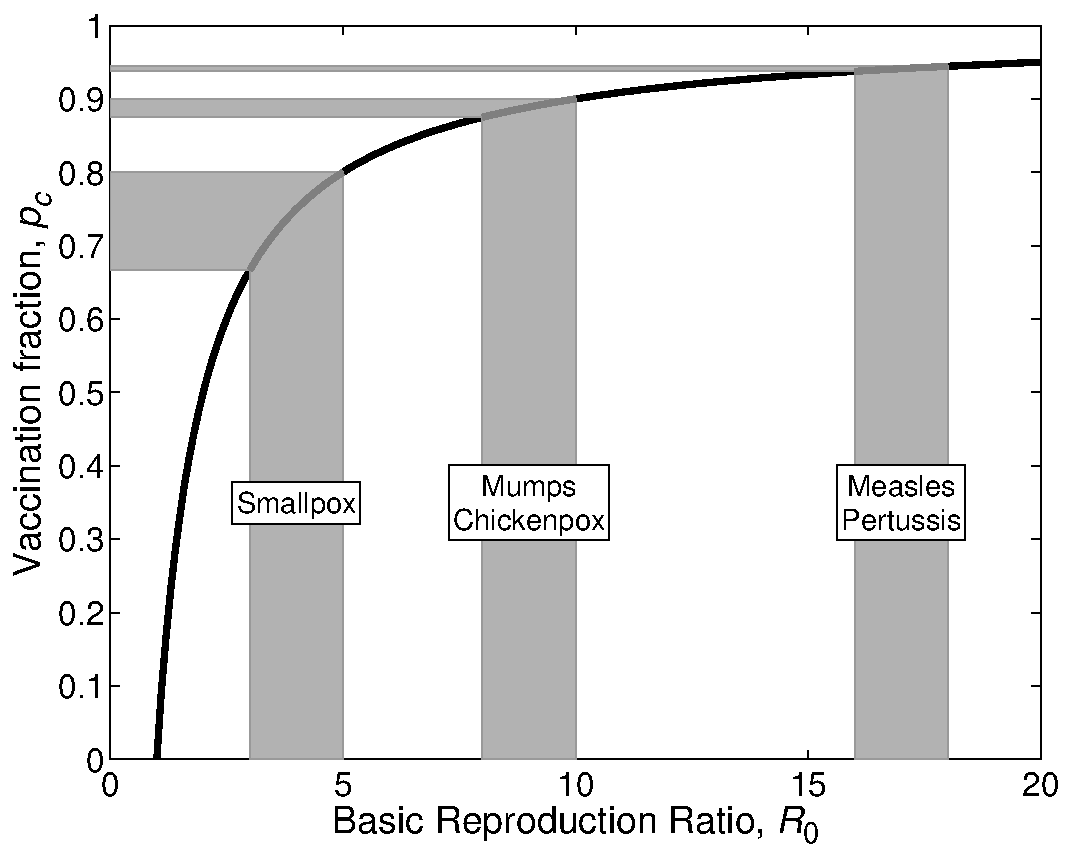
\includegraphics{./images/kr-R0intervention.pdf}
\caption{\label{fig:krR0intervention}R\textsubscript{0} and Interventions.
From (Keeling and Rohani \protect\hyperlink{ref-keeling08}{2008}).}
\end{figure}

\subsubsection{R and the SIR Model}\label{myadvancedbox}

We can connect the concept that R\textgreater{}1 leads to growth and
R\textless{}1 leads to a decline in infectious persons with the simple
SIR model for an outbreak. The model, which we saw earlier, is given by
the following set of differential equations (Don't confuse the \emph{R}
for the recovered with the R/R\textsubscript{0} from the reproductive
number. Unfortunately it is customary to use the same letter for both.):

\[ 
\begin{aligned}
\dot S &= - b SI \\
\dot I &= b S I - g I \\
\dot R &= g I
\end{aligned}
\] For this model, what needs to be true to get an increase in the
number of infectious hosts? The influx of new infectious hosts,
b\emph{S}I, needs to be larger than the outflow, g\emph{I. This
condition, b}S\emph{I \textgreater{} g}I, can be rewritten as 1
\textless{} (b\emph{S)/g. We then define the quantity on the right side
of this condition as the reproductive number, R = (b}S)/g. At the
beginning of an outbreak, where everyone is assumed to be susceptible
(written as S= S\textsubscript{0}), we have the special case of the
basic reproductive number, R\textsubscript{0} =
(b\emph{S\textsubscript{0})/g. Note that the rate of recovery, g, is
related to the average duration of infection, D as D=1/g. Therefore, one
can also write R = D}b*S, with the special case R\textsubscript{0} for
S=S\textsubscript{0}, i.e.~at the beginning of an outbreak.

\section{How to determine R -
Overview}\label{how-to-determine-r---overview}

Knowing the reproductive number for a particular pathogen and scenario
is important to allow for adequate intervention planning. There are
multiple ways to estimate R from data. We'll briefly discuss them now.

\section{Determine R at the Beginning of an
Outbreak}\label{determine-r-at-the-beginning-of-an-outbreak}

Very early in an outbreak, there will only be a few cases, and they
occur seemingly randomly/stochastically. If the outbreak continues
growing after a while, the case numbers will increase exponentially. The
exponential growth rate, r, can be estimated from the data, essentially
by fitting a straight line to the logarithmic values of the case report
data. To go from the growth rate to R, we need some further information.
Namely, we need to know the serial interval. The serial interval, T, is
the time between onset of infection in one host to the onset of
infection in a secondary host. Sometimes T can be approximated by the
duration of the infectious period, D.

Once we know r and T, we can compute R. There are different equations
relating r and T to R, they depend on specific assumptions one makes
about the disease. One relation between r, T, and R is given by R = 1 +
rT, and another one is given by R = e\textsuperscript{rT} . For
assumptions underlying these equations and further details, see e.g.
(Wallinga and Lipsitch \protect\hyperlink{ref-wallinga07}{2007}).

\begin{figure}
\centering
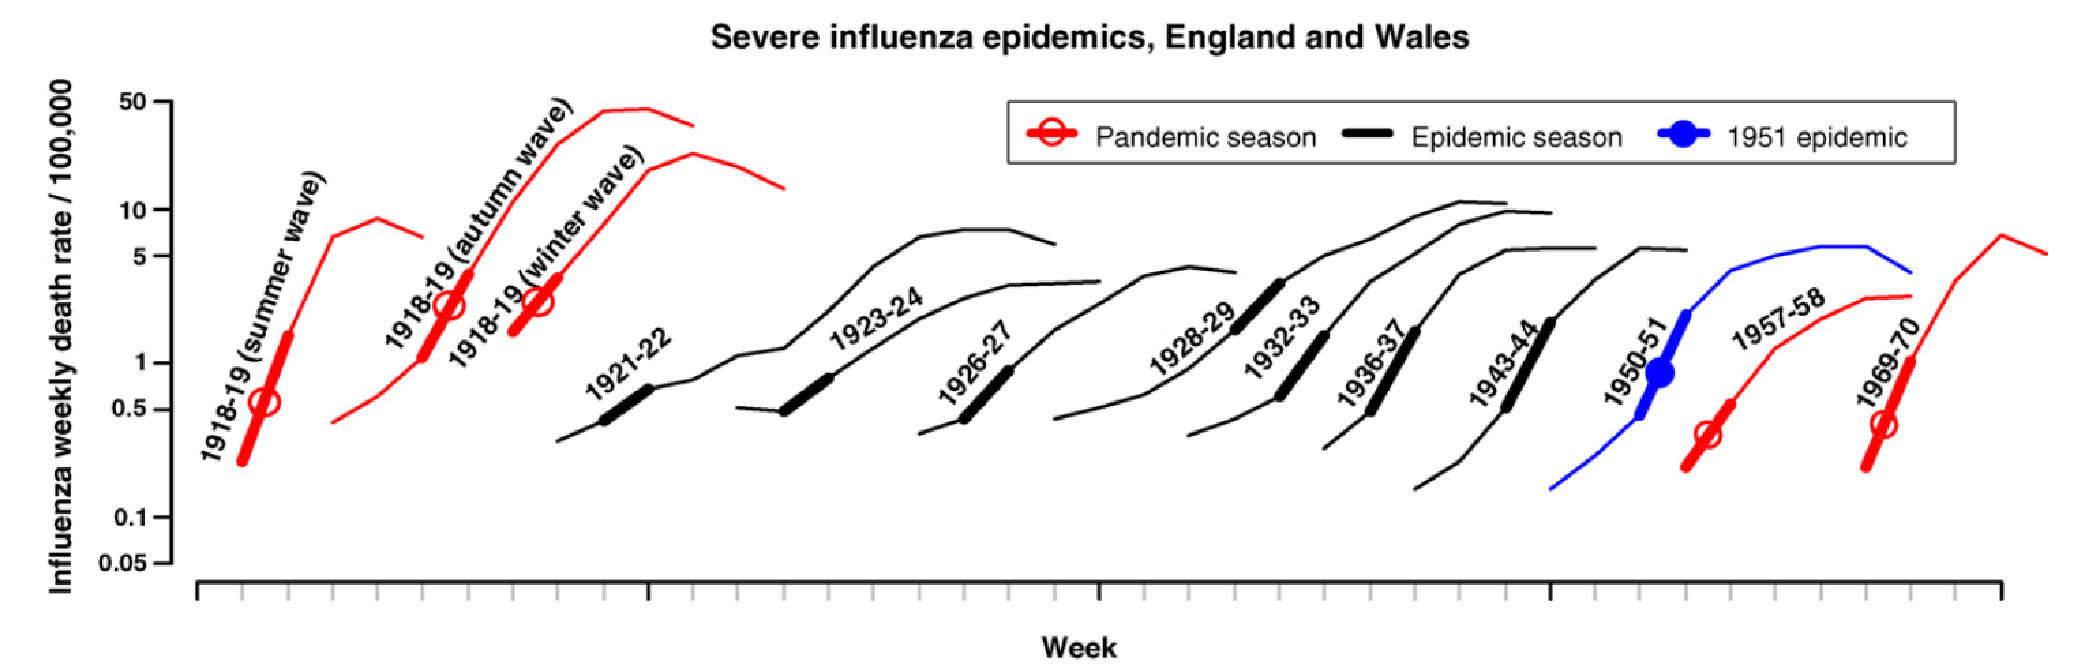
\includegraphics{./images/viboud-R0.pdf}
\caption{\label{fig:viboudR0}Example of R0 estimation based on case data in
the early stages of an outbreak. Source: Viboud et al 2006 Vaccine
(Viboud et al. \protect\hyperlink{ref-viboud06}{2006}).}
\end{figure}

\section{Determine R Once the Outbreak is
Over}\label{determine-r-once-the-outbreak-is-over}

A larger R leads to a larger outbreak (ignoring things like
interventions, behavior change, etc.). The reason to determine R is so
we can use it to predict the expected size of an (uncontrolled) outbreak
- and more importantly, we can learn how strong our intervention efforts
need to be. But we can also flip things around. Once an (uncontrolled)
outbreak has occurred, knowing the outbreak size can allow us to
estimate R. It is often possible to determine outbreak sizes after an
outbreak has occurred, e.g.~through serosurveys which show antibodies
against the disease and therefore indicate who got infected. We don't
need any `timing' information, just the fraction infected at the end.
Essentially, we need to know the number of people that got infected, and
the number of people who were at risk (i.e.~the susceptibles) at the
beginning of the outbreak. Once we know these pieces of the puzzle, we
can estimate R.

More specifically, assume we know the final size of the outbreak,
i.e.~total fraction of those becoming infected, I\textsubscript{f} =
I\textsubscript{tot}/N, where N is the population at risk and
I\textsubscript{tot} is the total number of infected. We then also know
the fraction of susceptibles that are left at the end of an outbreak,
S\textsubscript{f}=1-I\textsubscript{f}. To find R/R\textsubscript{0},
we can use the equation
R=\emph{ln}(S\textsubscript{f})/(S\textsubscript{f} - 1) (here,
\emph{ln} is the natural logarithm). The figure below shows the relation
between the fraction infected and R\textsubscript{0} graphically.

\begin{figure}
\centering
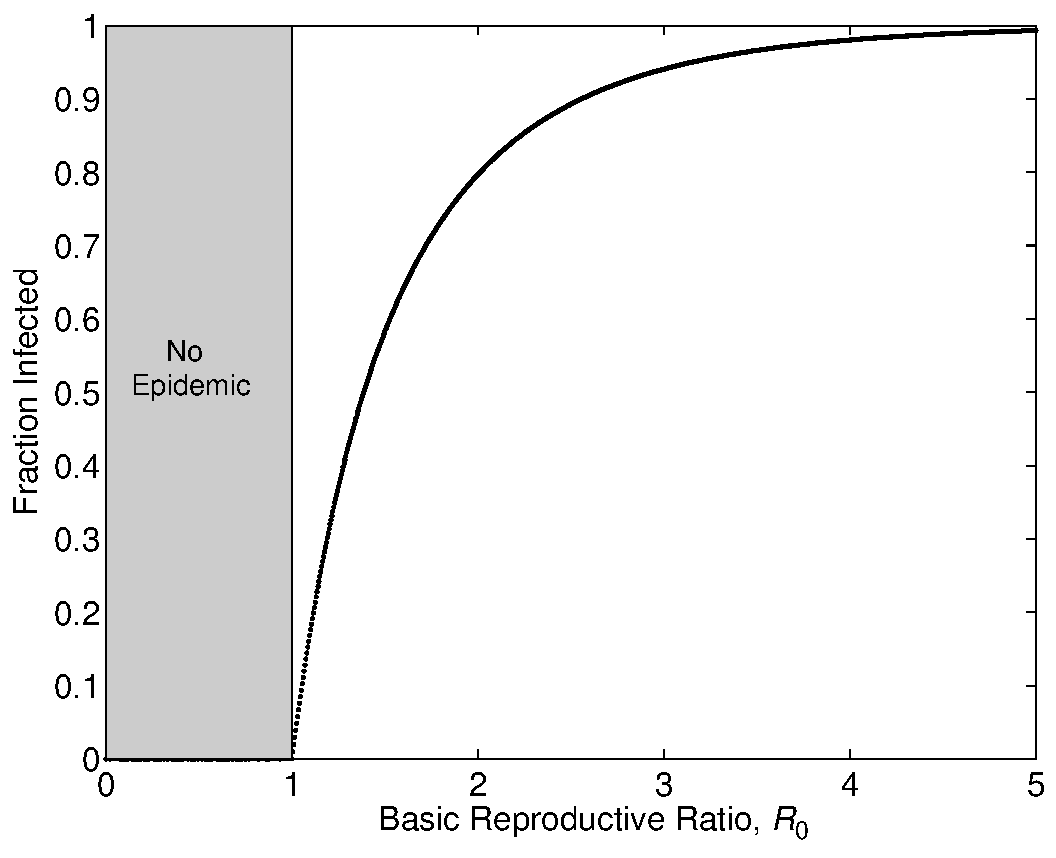
\includegraphics{./images/outbreaksize.pdf}
\caption{\label{fig:outbreaksize}The relation between R\textsubscript{0} and
outbreak Size. If we have information about the size of an outbreak (in
the absence of control measures), we can use it to estimate
R\textsubscript{0}. Source: Keeling and Rohani 2008 (Keeling and Rohani
\protect\hyperlink{ref-keeling08}{2008}).}
\end{figure}

For the above equation to be true, we assume that initially everyone is
susceptible and that the population is well mixed. More refined
estimates for R, with more complicated equations, are available (Ma and
Earn \protect\hyperlink{ref-ma06}{2006}).

\section{Determining R at the Endemic/steady
state}\label{determining-r-at-the-endemicsteady-state}

For an ID that is at an endemic/steady state, we have another way of
determining R\textsubscript{0}. At the endemic equilibrium, the
reproductive number is R\textsubscript{eq} = 1. If it weren't, the ID
would either grow or decline, and it wouldn't be the endemic state. At
this endemic state, a fraction of the population is still susceptible,
S\textsubscript{eq}. By definition, at the beginning of an ID with
transmissibility R\textsubscript{0}, everyone is susceptible
(S\textsubscript{0}=1, expressed as a fraction). If we know
S\textsubscript{eq}, we can then compute R\textsubscript{0} as given by
R\textsubscript{0} = R\textsubscript{eq}
S\textsubscript{0}/S\textsubscript{eq} = 1/ S\textsubscript{eq}. As an
example, if at an endemic state (with R\textsubscript{eq}=1), 50\% of
the population is susceptible, then at the beginning, when 100\% of the
population was susceptible, we have R\textsubscript{0}=2. Conversely, if
we know R\textsubscript{0}, we can predict the number of susceptibles at
the endemic state, S\textsubscript{eq}=1/R\textsubscript{0}.

\section{Determining R Through Age of
Infection}\label{determining-r-through-age-of-infection}

For those ID for which an infection induces life-long immunity,
i.e.~where a host can only be infected once, the age of infection is an
important concept. Intuitively, the more infectious a disease is, the
more likely it is that a host gets an ID at an early age. For an ID that
induces immunity, one can collect serological data (i.e.~antibody
measurements) to determine the fraction of individuals of a given age
who have antibodies, which means they have been previously infected
(assuming for the moment that no vaccine is available). One can define
the median age of infection as the age at which 50\% of the population
has been infected.

\begin{figure}
\centering
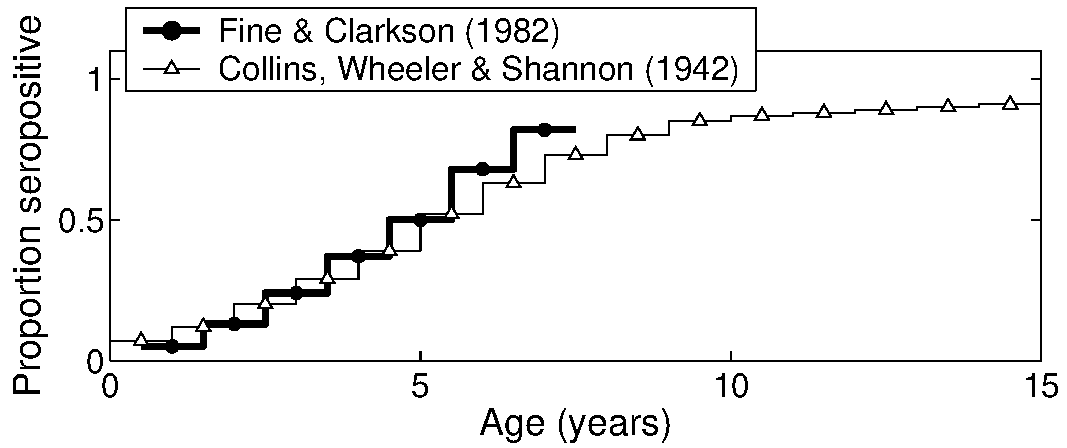
\includegraphics{./images/R0age.pdf}
\caption{\label{fig:R0age}Fraction seropositive (previously infected) as
function of age for measles. Source (Keeling and Rohani
\protect\hyperlink{ref-keeling08}{2008}).}
\end{figure}

For a simple model with certain assumptions (Keeling and Rohani
\protect\hyperlink{ref-keeling08}{2008}), one can find an approximating
equation connecting the median age of infection and the basic
reproductive number with the equation \(A \approx \frac {L}{R_0 - 1}\)
or rewritten \(R_0 \approx \frac{L}{A} + 1\). In this equation, \emph{L}
is the average life expectancy of a host and \emph{A} is the median age
of infection. This shows what we expect intuitively: Higher
R\textsubscript{0}, i.e.~more infectious ID, leads to an earlier age of
infection.

\emph{Note: If you want to determine R/R\textsubscript{0} to be used as
parameter in a mathematical transmission model, you use this approach
based on the age-seroprevalence relation even if the model you plan on
using doesn't have age in it.}

\section{Determining R Through Fitting a Full Transmission
Model}\label{determining-r-through-fitting-a-full-transmission-model}

Instead of just using data for the initial exponential growth phase,
determining \emph{r} and computing R\textsubscript{0} as specified
above, we can fit some or all outbreak data to an SIR type model. We use
the data to estimate the parameters of the model. For instance, for the
simple SIR model, we would estimate the transmission rate, b, and
recovery rate, g. We can then use the equation for R\textsubscript{0}
for a given model to compute its value. For the simple SIR model, that
would be R\textsubscript{0} = bS\textsubscript{0}/g.

\subsubsection{Computing R for a Given Model}\label{myadvancedbox}

Once a mathematical model for a given ID and setting has been specified,
it is often useful to compute R\textsubscript{0} for the model. Above,
we looked at one way to get R\textsubscript{0} for the basic SIR model,
i.e.~we determined that bS/g needs to be greater than 1 and that turned
out to be R\textsubscript{0}. However, it is often better to derive
R\textsubscript{0} for a given model by starting with the basic
definition: R\textsubscript{0} is the average number of secondary
infections caused by one infected individual, assuming the population is
fully susceptible. We can then reason as follows: An individual infected
person infects new susceptibles at a rate b S\textsubscript{0}, for a
duration of 1/g. Therefore the total number of newly infected
individuals is bS\textsubscript{0}/g. Let's apply the same reasoning to
a few variations of the SIR model. Consider the following SIR model with
an additional, disease-induced mortality at rate \emph{m}.

\[ 
\begin{aligned}
\dot S &= -b SI \\
\dot I &= b S I - g I - m I\\
\dot R &= g I
\end{aligned}
\]

An individual infected again infects at rate b\emph{S. The average
duration for which an individual is infectious is now 1/(g + m),
i.e.~the sum of all the outflows out of the \emph{I} compartment. That's
a general rule: The average duration of stay in a given compartment is
the inverse of the sum of all the outflows. Therefore, for this model,
we now get R\textsubscript{0} = b}S\textsubscript{0}/(g+m). Computing R
for larger models can get complicated. There are specific methods one
can use for more complex models. See for instance (Diekmann,
Heesterbeek, and Roberts \protect\hyperlink{ref-diekmann10}{2010}) for
further information on this.

\section{R and model
parameterization}\label{r-and-model-parameterization}

Knowing R is not only essential for public health intervention planning,
but it is also an important component of building and analysis of
infectious disease models. Most models have a parameter for the
transmission rate, such as \emph{b} in the models above. To allow
simulation of a model, all parameters need to get assigned specific
values - chosen to correspond to the disease and scenario under study.
Direct estimates of the transmission rate for a model are usually hard
to find. Instead, we often determine R/R\textsubscript{0} for a given
ID/setting and then use it to compute \emph{b} using equations like
those shown above.

\section{Summary and Cartoon}\label{summary-and-cartoon-3}

The reproductive number is a crucial concept in infectious disease
epidemiology. It has a relatively straightforward definition. However,
estimating R for a specific disease and scenario is not always easy.

Under the assumption that everyone is susceptible, the reproductive
number gets the special name \emph{basic reproductive number} and is a
denoted by R\textsubscript{0}. Knowing R/R\textsubscript{0} helps in
planning the scale of interventions.

R only measures one -- important -- component of a disease, namely its
transmission potential/transmissibility. For a full understanding of a
given disease, we need to know other characteristics such as speed of
transmission, the severity of disease including mortality, routes of
transmission, and other disease specific details.

The simplicity of R is both its strength and its weakness. It gives a
quick, quantitative assessment of the transmission potential (and
therefore outbreak size and needed control measures) of a disease.
However, R is a population level average and ignores heterogeneities of
host, agent, and environment. Therefore any R estimates are only
approximate.

\begin{figure}
\centering
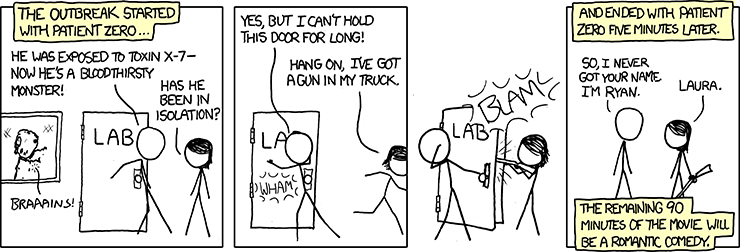
\includegraphics{./images/xkcd-outbreak-control.png}
\caption{\label{fig:xkcd-outbreak-control}The R\textsubscript{0} in this
case was 0. \href{https://xkcd.com/734/}{Source: xkcd.com}.}
\end{figure}

\section{Exercises}\label{exercises-3}

\begin{itemize}
\tightlist
\item
  The \emph{Reproductive Number} app in the DSAIDE package provides
  hands-on computer exercises for this chapter.
\item
  Find a paper from the research literature that provides evidence for
  herd immunity for a specific infectious disease and setting. Summarize
  the paper and explain how it demonstrates the occurrence of herd
  immunity.
\item
  Read the paper ``Herd Immunity: A Rough Guide'' by Fine et al. (Fine,
  Eames, and Heymann \protect\hyperlink{ref-fine11}{2011}). In this
  paper, the authors mention \emph{``\ldots{}the complexities of
  imperfect immunity, heterogeneous populations, nonrandom vaccination,
  and freeloaders\ldots{}''}. For each of those complexities, find, read
  and summarize a research paper that discusses the topic. Ideally,
  choose papers other than those already cited by Fine et al.
\item
  Compute R\textsubscript{0} following the scheme described in this
  chapter for the following model, which has an additional compartment
  of exposed, not-yet infectious hosts (we called those \emph{P} in
  previous models). Note that you always go ``full circle'', i.e.~from
  one infectious individual back to infectious individuals:
  \(\dot S = -b SI, \ \dot E = b S I - a E, \ \dot I = a E - g I - m I, \ \dot R = g I\).
\item
  Compute R\textsubscript{0} following the scheme described in this
  chapter for the following model, which includes births and deaths:
  \(\dot S =m - b SI - n S, \ \dot E = b S I - a E - n E, \ \dot I = a E - g I - n I, \ \dot R = g I - n R\).
  (Note that in the previous exercise, the parameter \emph{m} represents
  disease-induced mortality, here it represents births. I'm purposefully
  re-cycling it, so you get used to the fact that different
  papers/people use different letters for parameters. Always read
  carefully.)
\end{itemize}

\section{Further Resources}\label{further-resources-3}

\begin{itemize}
\tightlist
\item
  The following papers provide further discussions and details on the
  reproductive number: (Heffernan, Smith, and Wahl
  \protect\hyperlink{ref-heffernan05}{2005}; Roberts
  \protect\hyperlink{ref-roberts07}{2007}; Li, Blakeley, and Smith
  \protect\hyperlink{ref-li11}{2011}).
\item
  Further discussions regarding herd immunity can be found in (Metcalf,
  Edmunds, and Lessler \protect\hyperlink{ref-metcalf15}{2015}; Fine
  \protect\hyperlink{ref-fine93}{1993}).
\end{itemize}

\section{References}\label{references-4}

\chapter{Types of Infectious Disease
Transmission}\label{types-of-infectious-disease-transmission}

\section{Overview and Learning
Objectives}\label{overview-and-learning-objectives-4}

In this chapter, we will introduce different types of ID transmission
and how these different modes of transmission impact ID dynamics.
Several of the following chapters will go into more detail on different
modes of transmission.

The learning objectives for this chapter are:

\begin{itemize}
\tightlist
\item
  Know the different types of ID transmission
\item
  Understand the implications different modes of transmission have for
  ID dynamics and control
\end{itemize}

\section{Introduction}\label{introduction-4}

The way in which an infectious disease transmits is important to
understand its transmission dynamics and for planning interventions. An
infectious disease can be transmitted directly or indirectly. Among
indirect ways of transmission, there are again different important
categories, such as environmental or vector-borne transmission. Often,
things are not that clear-cut: Some diseases might transmit by more than
one route, and the definition of direct and indirect is not as clear-cut
as it might sound. The following paragraphs briefly discuss the main
different transmission modes, which will then be discussed in more
detail in the following chapters.

\section{Direct Transmission}\label{direct-transmission}

The most straightforward way of transmission is direct transmission from
infected to uninfected host. The clearest example of direct transmission
are sexually transmitted diseases. It is generally the case that direct
physical contact between infected and uninfected host is required for
transmission. Exceptions exist, such as transmission of HIV through
infected needle sharing, which could even be considered a type of
vector-borne transmission, but non-direct modes of transmission are not
common.

Respiratory diseases are often also considered to transmit directly if
close proximity between infected and uninfected host is needed for
successful transmission. Examples are measles and influenza. It gets a
bit tricky though since many respiratory pathogens can also transmit by
first being deposited in the environment (e.g., inside tiny water
particles floating in the air for a long time, or on a bathroom faucet).
Then if an uninfected person comes into contact with the contaminated
environment, they can get infected. The importance of direct versus
indirect/environmental transmission for many respiratory pathogens is
still not fully understood, and can likely differ between different
settings.

Another path of direct transmission is from mother to baby before or
during birth. This is often called \emph{vertical transmission}, while
all other forms discussed above and below are called \emph{horizontal
transmission}. HIV is an example of a pathogen that can transmit via
both routes.

\section{Environmental Transmission}\label{environmental-transmission}

As just mentioned, respiratory infections might spread through an
environmental stage, where the environment is small water particles in
the air or on solid surfaces. Infected surfaces (in the context of ID
transmission often called fomites) are major routes of transmission for
several important pathogens, for instance, Staph or pathogens that
transmit through the fecal-oral route, e.g., norovirus. Water is the
main transmission environment for another important fecal-orally
transmitted disease, Cholera. The chapter on environmental transmission
will discuss this route in more detail.

\section{Vector-borne Transmission}\label{vector-borne-transmission}

Diseases that transmit through a vector stage, such as Malaria, Dengue,
Zika, and others, are an important category. The most common and
important vector are mosquitos, but other vectors are also important
(e.g., kissing bugs for Trypanosoma, which causes Chagas disease). The
definition of what makes an ID a vector borne ID is tricky. See the
HIV-needle example above, or consider Zika, which can transmit by
multiple routes. For some diseases, it is not clear if one should
consider them vector-borne or not. For instance, \emph{Toxoplasma
gondii} spends part of its life-cycle in cats, and the other part can be
in another host, most commonly mice or birds. If the latter type of host
should be considered a vector or not is largely a matter of definition.
Often, it is called an intermediate host, and \emph{T gondii} and
diseases with similar life-cycles (e.g., Schistosomiasis) are considered
\emph{multi-host diseases}, with the term vector-borne mainly used when
the intermediate (non-human) host is an insect. As we will see, from the
perspective of describing such diseases with models, the labeling does
not make much of a difference.

\section{Summary and Cartoon}\label{summary-and-cartoon-4}

This chapter briefly introduced different modes of ID transmission.

\begin{figure}
\centering
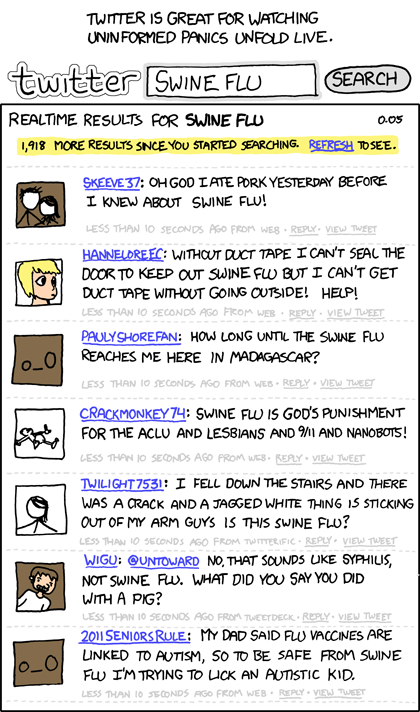
\includegraphics{./images/xkcd-swine_flu.png}
\caption{Knowing transmission routes is important to understand how one
can and cannot contract a specific disease.
\href{https://xkcd.com/574/}{Source: xkcd}}
\end{figure}

\section{Exercises}\label{exercises-4}

\begin{itemize}
\tightlist
\item
  Several apps in the DSAIDE package address specific types of
  transmission, those are discussed in the following chapters.
\end{itemize}

\section{Further Resources}\label{further-resources-4}

\begin{itemize}
\tightlist
\item
  Ewald and colleagues have done some interesting investigations
  connecting transmission type to virulence/pathogenicity of specific
  diseases. See for instance (Ewald
  \protect\hyperlink{ref-ewald87}{1987}; Ewald
  \protect\hyperlink{ref-ewald95}{1995}).
\item
  A detailed discussion linking transmission types to model alternatives
  is provided in (McCallum et al.
  \protect\hyperlink{ref-mccallum17}{2017}).
\end{itemize}

\section{References}\label{references-5}

\chapter{Modes of Direct
Transmission}\label{modes-of-direct-transmission}

\section{Overview and Learning
Objectives}\label{overview-and-learning-objectives-5}

In this chapter, we will discuss different types of direct transmission
and explore how these different modes of transmission impact ID
dynamics.

The learning objectives for this chapter are:

\begin{itemize}
\tightlist
\item
  Understand the assumptions underlying different modes of direct
  transmission
\item
  Understand how different modes of direct transmission affect ID
  dynamics
\end{itemize}

\section{Introduction}\label{introduction-5}

The direct transmission of a pathogen means it goes straight from an
infected host to a new uninfected host. Sounds simple enough, but as
we'll discuss here \emph{straight from host to host} is in fact not that
straightforward, and many pathogens have both direct and indirect
transmission components. We'll discuss the most important direct
transmission types and what hosts fall under that umbrella.

\section{Contact transmission}\label{contact-transmission}

The most straightforward way of transmission is through direct contact
between infected and uninfected hosts. A prime class of pathogens that
follow this route are sexually transmitted infections (STI). For STIs,
the pathogen goes directly from one host to the other. Another pathogen
for which direct contact is an important (but not the only) route of
transmission is Ebola.

A particular group of contact transmission is vertical transmission
between mother and child. This type of transmission is important for
diseases such as HIV or Ebola. Since a model system for vertical
transmission will, at the minimum, require stratification by age, it
will not be discussed further here. After reading the \href{}{\emph{Host
Heterogeneity} chapter}, it should be clear how such a scenario could be
modeled.

\section{Airborne transmission}\label{airborne-transmission}

Some pathogens are \emph{essentially direct} with only a very short time
spent outside the host. Many respiratory infections fall in this
category. Those pathogens are often expelled as small air drops by the
host (through breathing, sneezing or coughing) and then are quickly
inhaled by an uninfected host, thus potentially causing a new infection.
Similarly, a pathogen might for a brief time be deposited on a surface
(e.g., a bathroom faucet). Such a potentially infected surface is often
called a fomite. If the pathogen is picked up fairly quickly by an
uninfected host and thus completes the transmission process, it is
sometimes also reasonable to consider this an essentially direct
transmission process.

The decision to consider airborne or surface mediated transmission
direct or indirect transmission is very much dependent on the
perspective and focus of the question one wants to address. For some
questions and situations, assuming this route of transmission to be
essentially direct is reasonable. For instance, for a large-scale
simulation of a flu pandemic, it is usually a reasonable assumption to
consider transmission directly between infected and uninfected hosts,
without explicitly considering an environmental stage. In contrast, if
one wants to study the transmission process in detail, it might be
necessary to consider the short time the pathogen explicitly spends in
the environment and thus using the perspective discussed in the
\emph{Environmental Transmission} chapter.

\section{Ways in which direct transmission
scales}\label{ways-in-which-direct-transmission-scales}

For direct transmission, there are important ways in which transmission
can scale with population size or population density. One often
distinguishes between \emph{density-dependent} and
\emph{frequency-dependent} transmission. Unfortunately, the terminology
is not very consistent. Other terms are used and sometimes misused. See,
e.g. (McCallum, Barlow, and Hone
\protect\hyperlink{ref-mccallum01}{2001}, Begon et al.
(\protect\hyperlink{ref-begon02}{2002})) for a discussion of this.

The main differences between these two types of transmission have to do
with the scaling of transmission intensity (often measured by the force
of infection) as population size changes. This is a feature of the
number of contacts that a susceptible has with an infected person. For
some types of ID, e.g., STI, the number of contacts (i.e., sexual
encounters) is likely not too dependent on the population density or
size. For instance, the average person living in a town of 100,000
people likely has pretty much the same number of sexual contacts
compared to the person living in a town of 1 million. One could argue
that more opportunities might lead to more sexual contacts, but it's
unlikely to change by much. This type of invariance of transmission is
labeled (using the terminology of (McCallum, Barlow, and Hone
\protect\hyperlink{ref-mccallum01}{2001},Begon et al.
(\protect\hyperlink{ref-begon02}{2002}))) \emph{frequency-dependent}.

In contrast, for some ID, more individuals (given a constant area) leads
to more contacts and more transmission. This might apply to ID such as
influenza or norovirus. A scenario where an increase in population
size/density leads to a (linear) increase in transmission is usually
referred to as \emph{density-dependent} transmission. However, even for
ID that do show some signs of density dependence, the number of social
contacts often dominates. For instance, a person in a city that is 10
times the size of a smaller city likely won't have 10 times as many
contacts.

\subsection{Modeling types of direct transmission}\label{myadvancedbox}

Assuming the simple SIR model, we have the set of equations \[ 
\begin{aligned}
\dot S &= - \lambda S \\
\dot I &= \lambda S  - \gamma I \\
\dot R &= \gamma I.
\end{aligned}
\] The \emph{force of infection}, \(\lambda\) - is equal to \emph{bI}.
The force of infection can be rewritten in a different form, namely
\(\lambda= cpv\), where \emph{c} is the rate of contacts between hosts,
\emph{p} is the probability that a contact is with an infected host and
\emph{v} is the probability that transmission occurs during contact. As
an example, for HIV, \emph{c} would measure the frequency of sexual
encounters, \emph{p} would quantify the fraction of those encounters
that happen with an HIV+ individual, and \emph{p} quantifies the
probability that having sex with an HIV+ individual leads to infection.

Now, depending on the specific assumptions we make for the different
parameters, we can end up with different types of transmission. We often
assume that the probability that a contact is with an infected host is
equal to the prevalence of the ID in the population, i.e., p = I/N. This
is the so-called well-mixed population assumption and holds for both
frequency- and density-dependent SIR type models. If we wanted to relax
this assumption, we would need to switch to for instance network-based
models or build more complicated compartmental models.

For density-dependent transmission, we assume that the rate of contacts
is proportional to the density of hosts, i.e., c = kN/A, where N is the
population size and A the area, and k is some constant of
proportionality. As stated above, this might be a good approximation for
some ID and scenarios, e.g., influenza.

For frequency-dependent transmission, we assume that the rate of
contacts is fixed and independent of the density of hosts, i.e., c = f.
This might be a good approximation, e.g., sexually transmitted diseases,
where the number/density of individuals in the vicinity of an individual
does not (or only in a small way) influence the rate at which a person
has sexual contacts. We therefore end up with \(\lambda_d= kv I/A\) and
\(\lambda_f= fv I/N\) for density- and frequency- dependent
transmission. The terms \emph{kv} and \emph{fv} are often combined into
a new parameter, \emph{b\textsubscript{d}} and
\emph{b\textsubscript{f}}. If population size and area are fixed, the
transmission types lead to the same results, as long as parameter values
are chosen accordingly. If population size changes (not uncommon) or
area changes (less common), one needs to be more careful with the choice
of transmission term.

\section{Summary and Cartoon}\label{summary-and-cartoon-5}

This chapter described different assumptions for direct transmission
models and how they lead to different results with regard to disease
dynamics and potential control strategies.

\begin{figure}
\centering

\includegraphics{./images/smbctransmissionmode.png}
\caption{Some pathogens have direct and more indirect modes of
transmission. \href{http://www.smbc-comics.com/}{Source:
smbc-comics.com}}
\end{figure}

\section{Exercises}\label{exercises-5}

\begin{itemize}
\tightlist
\item
  The \emph{Direct transmission} app in the DSAIDE package provides
  hands-on computer exercises for this chapter.
\item
  Read the paper ``How should pathogen transmission be modelled?'' by
  McCallum et al. (McCallum, Barlow, and Hone
  \protect\hyperlink{ref-mccallum01}{2001}). The authors discuss
  different models for (direct) transmission. They claim that it matters
  in a practical setting to get the transmission term right. Pick some
  ID and explain how different assumptions about transmission might lead
  to different conclusions concerning possible control strategies.
\end{itemize}

\section{Further Resources}\label{further-resources-5}

\begin{itemize}
\tightlist
\item
  The paper (Begon et al. \protect\hyperlink{ref-begon02}{2002})
  provides some additional information and discussion on the topic of
  direct transmission types and how they should be modeled.
\item
  In (Ferrari et al. \protect\hyperlink{ref-ferrari11}{2011}), the
  authors discuss transmission scaling and connect it to network models.
  (This book briefly discusses networks in the \emph{Networks }
  chapter).
\end{itemize}

\section{References}\label{references-6}

\chapter{Environmental Transmission}\label{environmental-transmission-1}

\section{Overview and Learning
Objectives}\label{overview-and-learning-objectives-6}

A number of pathogens are transmitted through an environmental stage.
This chapter discusses the implications on the ID dynamics in such
cases.

The learning objectives for this chapter are:

\begin{itemize}
\tightlist
\item
  Know the hallmarks of indirect, environmental transmission
\item
  Understand what environmental transmission implies for control
  strategies
\item
  Identify diseases for which the environmental transmission pathway is
  important
\end{itemize}

\section{Introduction}\label{introduction-6}

While the distinction between direct and indirect transmission is not
clear-cut, we usually consider an ID to have an indirect mode of
transmission if the time spent outside the main host is \emph{important}
for the whole transmission cycle. The two main types of stages where a
pathogen resides outside the main host are the abiotic environment or
another host species. In the case of the former, we consider it to be
environmental transmission, in the case of the latter, it is
vector-borne. Of course, some IDs are even more complicated and have
both vector and environmental stages. This chapter focuses on
environmental transmission.

\subsection{Environmental
transmission}\label{environmental-transmission-2}

Some diseases are shed by hosts into the environment, where they can
survive for a potentially extended time before re-infecting a new host.
Cholera is an excellent example of an ID that has water sources as the
environmental stage. Similarly, avian influenza is thought to survive in
cold lake water for an extended time. The important consequence of
environmental transmission is that it potentially allows new infections
to occur over long distances in time and space. For instance, an
infected person might shed Cholera into the water somewhere upstream,
and a susceptible person ingests the Cholera bacteria somewhere miles
downstream and days or weeks later. This is fundamentally different to
direct transmission, which requires close contact.

\begin{figure}
\centering
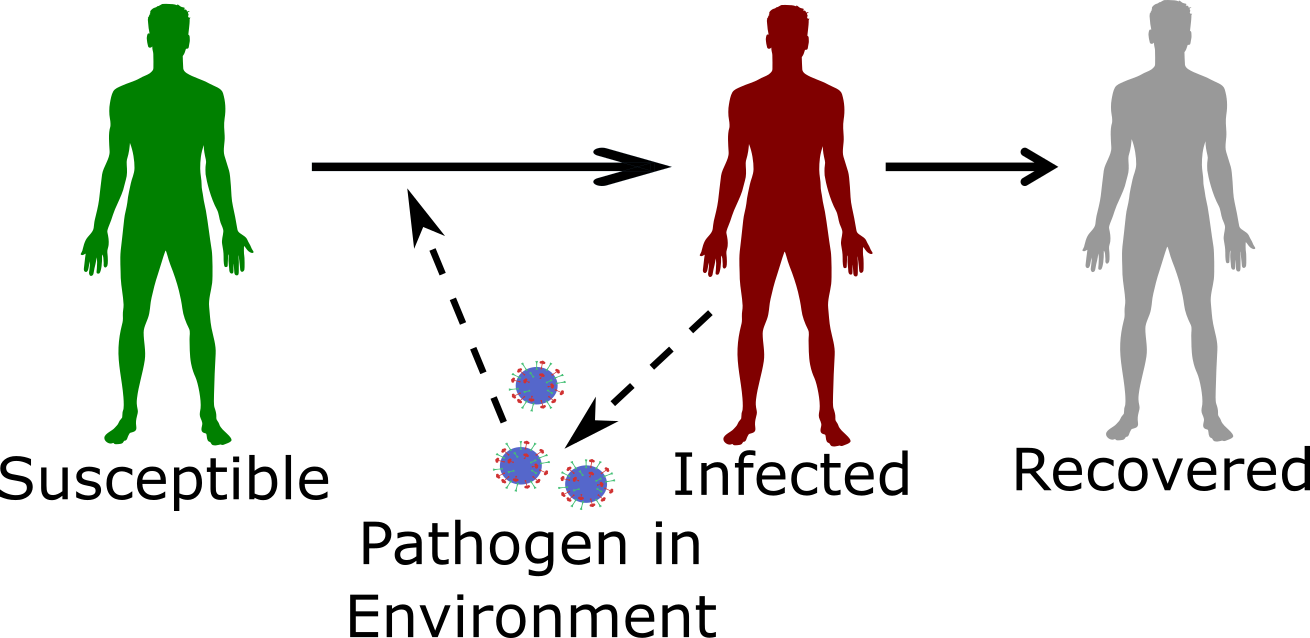
\includegraphics{./images/environmentaltransmissionscheme.png}
\caption{Schematic of an ID with environmental transmission}
\end{figure}

\subsection{Environmental transmission and external
drivers}\label{environmental-transmission-and-external-drivers}

Because environmental transmission involves the survival of pathogen for
a potentially extended time in the environment, such IDs are often more
strongly influenced by external drivers compared to IDs that are
directly transmitted. The weather often has a strong impact, as do
behavior changes. E.g., humans living in temperate zones are more likely
to swim in lakes when it's warm. Therefore water-borne diseases often
have the highest incidence in warm months.

Such external drivers can be included in models by allowing certain
parameters to vary over time. For instance the transmission rate or the
rate at which environmental pathogen decays could be made dependent on
the time of the year.

\subsection{Environmental transmission and
interventions}\label{environmental-transmission-and-interventions}

The environmental stage is a potentially great target for control
mechanisms. Disinfecting surfaces with chemicals such as bleach is
common practice in hospitals and other places where contamination might
be common and needs to be minimized. Similarly, attempts have been made
to disinfect the air with for instance UV radiation. Unfortunately, such
radiation can be harmful to humans, and thus this approach only works
within a system that moves and circulates air (e.g., an air-conditioning
system with a stage at which the circulated air is irradiated). All
modern water treatment plants have systems that remove pathogens, in
conjunction with good sanitation practices, have reduced the incidence
of diseases like Cholera. However, in developing countries, Cholera and
other water borne disease are still a major public health concern. Even
with proper sanitation, other pathogens like norovirus are hard to
control and still often cause local outbreaks. One reason for that is
that these viruses are hard to kill and many regular cleaning agents do
not work. Maybe the most important and famous environmental control
strategy is the tried and true method of hand washing. Our hands can be
considered a potentially infected environment (a fomite). By washing
them, the transmission of pathogens to others is minimized. The fact
that hand-washing is a great infection control strategy has been known
for centuries. Unfortunately, compliance is often still low, leading to
many needless infections, even in settings like hospitals, where one
should expect the staff to know the importance of adhering to the
hand-washing routine.

\subsubsection{Modeling environmental transmission}\label{myadvancedbox}

Most often, during the environmental stage, we assume that the pathogen
does not `do' anything. This is in contrast to vector-borne transmission
where the pathogen might, for instance, undergo replication in the
vector. Thus, we assume that infected hosts shed pathogen into the
environment, where it decays. If a susceptible person comes into contact
with the pathogen in the environment, an infection can occur. The
simplest SIR type model that can capture this process is given by \[ 
\begin{aligned}
\dot S &= - b E S \\
\dot I &= b E S  - \gamma I \\
\dot R &= \gamma I \\
\dot E &= p I - cE
\end{aligned}
\] Infected persons release pathogen into the environment at rate
\emph{p}. The pathogen decays at rate \emph{c}. A susceptible host can
get infected by contact with a contaminated environment at rate
\emph{b}.

\section{Summary and Cartoon}\label{summary-and-cartoon-6}

This chapter provided a discussion of environmental transmission and its
impact on ID dynamics and control.

\begin{figure}
\centering
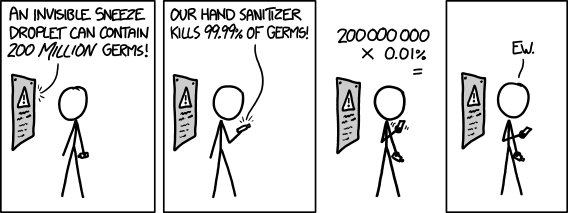
\includegraphics{./images/xkcd-hand_sanitizer.png}
\caption{One problem with environmental transmission control.
\href{https://xkcd.com/1161/}{Source: xkcd}}
\end{figure}

\section{Exercises}\label{exercises-6}

\begin{itemize}
\tightlist
\item
  The \emph{Environmental transmission} app in the DSAIDE package
  provides hands-on computer exercises for this chapter.
\item
  The paper by Killingley and Nguyen-Van-Tam describes modes of
  transmission for influenza. Pick a pathogen that can transmit in a
  somewhat similar manner (e.g., Ebola, SARS, MERS, or such) and compare
  and contrast what is known about similarities and differences in
  transmission between flu and the pathogen you pick. Also briefly
  discuss implications for control.
\end{itemize}

\section{Further Resources}\label{further-resources-6}

\begin{itemize}
\tightlist
\item
  The paper (Cortez and Weitz \protect\hyperlink{ref-cortez13}{2013})
  discusses how direct versus indirect transmission can lead to
  different incidence patterns and how models can help to determine
  routes of transmission.
\item
  Ewald discusses the relation between environmental transmission and
  virulence in (Ewald \protect\hyperlink{ref-ewald91}{1991}).
\item
  Some further discussion about influenza routes of transmission is
  provided in (Brankston et al.
  \protect\hyperlink{ref-brankston07}{2007}; Weber and Stilianakis
  \protect\hyperlink{ref-weber08}{2008}).
\end{itemize}

\section{References}\label{references-7}

\chapter{Vector-borne ID
Transmission}\label{vector-borne-id-transmission}

\section{Overview and Learning
Objectives}\label{overview-and-learning-objectives-7}

In this chapter, we will discuss an important form of indirect
transmission, one that has a vector stage.

The learning objectives for this chapter are:

\begin{itemize}
\tightlist
\item
  Know about important IDs that are vector-borne
\item
  Understand the implications of vector-borne transmission on ID
  dynamics
\item
  Understand how vector-borne transmission influences potential ID
  control strategies.
\end{itemize}

\section{Introduction}\label{introduction-7}

Vector-borne IDs are those that go through - at least - two different
hosts to complete a full replication and transmission cycle. Hosts of
one type infect hosts of the other, and there is no direct transmission
between hosts of the same type.

\begin{figure}
\centering
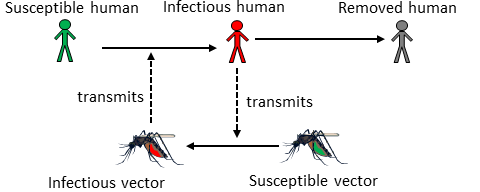
\includegraphics{./images/vectorborne-schematic.png}
\caption{Schematic of a vector-borne ID}
\end{figure}

Not surprisingly, the IDs which receive the most study are those where
one of the hosts are humans. The other host (i.e., the vector) can be
any other animal, such as dogs, rodents, snails, insects, etc. At times,
growth and replication of the pathogen occur mainly in one host, with
the other just serving as a vessel to get between hosts. Most often, the
pathogen completes significant parts of its growth and replication cycle
in both (or all, if there are more than 2) hosts.

\subsection{Vector-borne transmission and ID
patterns}\label{vector-borne-transmission-and-id-patterns}

Understanding what mechanisms lead to potentially observed patterns in
incidence and prevalence for vector-borne diseases is difficult, due to
the presence of more than one host. In a previous chapter, we discussed
cycles that could be caused by the intrinsic transmission dynamics or
influenced by external drivers (e.g., seasonal changes in weather). This
general concept still holds, but there are now two species (e.g., humans
and mosquitos), both have distinct and intrinsic dynamics and responding
differently to external factors. This obviously adds a lot of complexity
to the model. Nevertheless, patterns in ID dynamics are often observed
for vector-borne diseases and are at least partially understood. For
instance, the reproductive cycle of mosquitos strongly depends on the
weather, and specifically the availability or lack of water. As such, in
regions that have strong differences in rainfall between seasons, one
often observes annual cycles based on annual weather patterns.

\subsection{Vector-borne transmission and
interventions}\label{vector-borne-transmission-and-interventions}

With vector-borne ID, there is a unique opportunity for interventions
that do not exist for directly transmitted diseases. Namely, we can try
to control the ID at the vector stage. That often means trying to kill
as many vectors as possible. DDT in the past and more recently
pesticide-coated bed nets have been proven to work very effectively.
Unfortunately, these interventions need to be sustained. Otherwise,
mosquito numbers (or other vectors with a short lifespan) quickly bounce
back. Also, while we mostly think of mosquitos and other insects as a
nuisance or worse, they do perform important roles in the ecosystem, and
it is unclear what the consequences would be of potentially killing all
Anopheles mosquitos (they transmit a lot of important IDs). Some recent
approaches try to make mosquitos resistant to ID. If one could introduce
those and have them out-compete the mosquitos that are susceptible to
the ID, one might - in theory - get rid of relevant IDs without
affecting the ecosystem in unpredictable ways.

A major problem with all control strategies targeting vectors is that
not only do pathogens evolve quickly, but most vectors have fairly short
life spans and large population numbers, which means rapid evolution.
That could result in wide spread resistance making any control measures
ineffective within a short time. Indeed, that was observed for DDT,
where mosquitos resistant to the chemical started to appear before its
widespread use was discontinued.

\section{Modeling vector-borne transmission}\label{myadvancedbox}

The easiest way to model a vector-borne disease is to simply ignore the
vector and assume that the transmission term of the equation (e.g., a
term like \emph{bSI}) represents -- in a very simplified form -- all the
complicated processes involved in transmission, including the vector
stage. That makes the model simple, but of course, doesn't capture the
vector-borne aspects of the dynamics. If we are interested in the
dynamics of the disease in all hosts, we do need to include the vector
components in a model. To add vectors in a model, one could, for
instance, build 2 SIR-type models, with one set of equations for the
(human) host and one for the vector, and then couple the compartments by
including transmission from humans to vectors and vectors to humans.
Equations for such a model might look as follows: \[
\begin{aligned}
\dot S_h &= - \beta_1 S_h I_v \\
\dot I_h &= \beta_1S_h I_v - \gamma_h I_h \\
\dot R_h &= \gamma_h I_h \\
\dot S_v &= - \beta_2 S_v I_h \\
\dot I_v &= \beta_2 S_v I_h - \gamma_v I_v \\
\dot R_v &= \gamma_v I_v
\end{aligned}
\] Here, the index \emph{h} indicates humans and \emph{v} indicates
vectors. The important vector-borne aspect of such a model is that
transmission only occurs from hosts to vector and vector to host, not
between hosts or vectors. In general, the above model needs to be
modified to more accurately describe vector-borne ID dynamics. For
instance, many vectors have a fairly short natural lifespan, and as such
their births and deaths need to be included in the model, even if the
timescale in which we investigate the model is short enough to allow us
to ignore births and deaths for (human) hosts. It is common to include
more details in the human part of the model (e.g., asymptomatic stage
and others as discussed previously) and less detail for the vector part.
The specific details that should be included are driven by the question
one wants to study.

\section{Summary and Cartoon}\label{summary-and-cartoon-7}

Vector-borne transmission adds complexity to an ID, but also allows for
a wider range of control measures (such as vector killing).

\begin{figure}
\centering
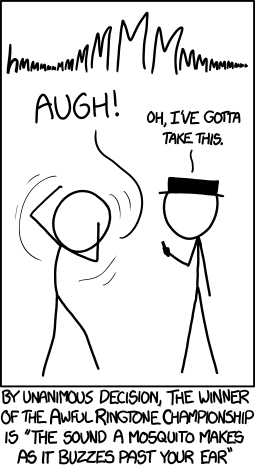
\includegraphics{./images/xkcd-mosquito-ringtone.png}
\caption{There are multiple reasons mosquitos are not popular.
\href{https://xkcd.com/1241/}{Source: xkcd}}
\end{figure}

\section{Exercises}\label{exercises-7}

\begin{itemize}
\tightlist
\item
  The \emph{Vector transmission} app in the DSAIDE package provides
  hands-on computer exercises for this chapter.
\item
  Nominate an ID as a contender for having the `craziest or most
  complicated' mode(s) of transmission. Explain the transmission
  dynamics for your nomination and justify why it deserves the title of
  \emph{craziest or most complicated}. This doesn't have to be a
  vector-borne disease, though some of the ``crazy'' ones tend to use
  multiple hosts.
\end{itemize}

\section{Further Resources}\label{further-resources-7}

\begin{itemize}
\tightlist
\item
  The following papers provide some additional discussion of
  vector-borne diseases and how to model them (Smith et al.
  \protect\hyperlink{ref-smith14}{2014}; Kilpatrick and Randolph
  \protect\hyperlink{ref-kilpatrick12}{2012}; Luz, Struchiner, and
  Galvani \protect\hyperlink{ref-luz10}{2010}).
\end{itemize}

\section{References}\label{references-8}

\chapter{Infectious Disease Control}\label{infectious-disease-control}

\section{Overview and Learning
Objectives}\label{overview-and-learning-objectives-8}

In this module, we will look a closer look at different types of control
against infectious diseases and their potential outcomes.

The learning objectives for this chapter are:

\begin{itemize}
\tightlist
\item
  Know the major types of ID control strategies
\item
  Evaluate the use of different ID control strategies
\item
  Understand how different pathogens require different types of control
\end{itemize}

\section{Introduction}\label{introduction-8}

Generally, the reason why we study IDs and their dynamics is to
eventually \emph{do something}. We want to implement control and
intervention strategies to minimize disease burden. That could be trying
to contain an ongoing outbreak, reduce the incidence of an endemic
disease, or try to eradicate a disease. Depending on modes of
transmission, infectiousness profiles and other ID characteristics, the
types of interventions that are available and potentially useful will
vary. Therefore, the better we understand and ID, the better we can
likely implement control.

\section{Goals of ID Control}\label{goals-of-id-control}

When trying to control an ID, we often have more than one goal in mind.
The following are a list of (overlapping) public health goals that we
often try to achieve with ID control:

\begin{itemize}
\tightlist
\item
  Reduce morbidity
\item
  Reduce mortality
\item
  Reduce transmission
\item
  Reduce incidence/prevalence
\item
  Reduce economic impact
\item
  Minimize ethical or moral dilemmas
\item
  Protect the individual
\item
  Protect the population
\end{itemize}

Most of these goals are overlapping. E.g., reducing transmission likely
reduces overall morbidity and mortality. Sometimes, goals can be
conflicting. For instance, if we have limited resources, should we
target those that are most likely to transmit but not suffer much from
the disease (e.g., children) or target those that are most likely to
experience morbidity/mortality but are not that necessary for
transmission (e.g., elderly)? Similarly, at what level is it acceptable
to force people to (not) do something (e.g., forced vaccination or
quarantine) that might not help - and maybe even slightly hurt - the
individual, but will be beneficial to society? Answers to those
questions are usually beyond the scope of just ID Epidemiology. What we
can contribute to the wider discussion is an assessment of the impact of
various control strategies. That information can then be combined with
other considerations to make decisions.

\section{Types of Infectious Disease
Control}\label{types-of-infectious-disease-control}

The types of control and intervention strategies that exist for a given
ID vary. Some depend on the route of transmission. Others depend on our
skills and ability, e.g., our ability to produce a vaccine. The
following sections describe the major types of ID control.

\subsection{Vaccination}\label{vaccination}

Vaccines are arguably the most cost effective public health intervention
we have. An ideal vaccine is one that has only to be given once to
induce lifelong protection against the ID. It should also be safe, with
little to no side effects. Other characteristics of a good vaccine are
ease of administration, low price and easy to transport and store.

The only IDs we have been able to eradicate so far (smallpox and
rinderpest) are those against which we have good vaccines.
Unfortunately, a good vaccine alone does not mean eradication is likely.
Measles is a good example. We have a good vaccine, but the pathogen is
so highly transmissible that coverage would need to be at levels beyond
those currently achievable.

\subsection{Pharmaceutical Interventions
(Drugs)}\label{pharmaceutical-interventions-drugs}

Drugs, most notably antibiotics, are another very effective means of
combating ID. While vaccines try to prevent infection, drugs usually try
to prevent symptoms (morbidity and mortality) in already infected
individuals. Reduction in symptoms might or might not impact
transmission dynamics. A good example where treatment reduces
infectiousness and transmission is ART treatment for HIV infected
individuals.

While not commonly used, drugs can also be given to susceptibles as
prophylaxis to reduce the risk of infection. As such, one can think of
drugs as short-term vaccines though the mechanism of protection is very
different. Again, HIV is a case in point, where pre-exposure prophylaxis
with ART has recently been shown to be somewhat effective in reducing
the risk of infection.

For some IDs, such as, helminth infections, mass drug treatment is also
being used to try and reduce ID prevalence enough to interrupt
transmission and potentially eliminate the ID.

\subsection{Non-pharmaceutical
Interventions}\label{non-pharmaceutical-interventions}

These are the oldest types of interventions and are often quite
effective. Quarantining of either infected or susceptibles prevents
further transmission. Quarantine alone does not help those that are
already infected. Though if quarantine occurs in a medical setting,
targeted help for the sick might reduce their morbidity and mortality. A
prominent recent example for the use of quarantine was during the 2014
Ebola outbreak in West Africa. No drugs or vaccines were available, and
quarantine was the main control strategy.

These days, strict quarantine can be hard to enforce, especially for
diseases that are not as severe as Ebola. A broader class of
intervention strategies, of which quarantine is a strong form, often
goes by the name of \emph{social distancing interventions}. E.g.,
closing a school to stop an ongoing flu or measles outbreak would
usually not be labeled as quarantine, but would be considered
\emph{social distancing}. In general, social distancing interventions
try to reduce mixing of infected and susceptible people, usually without
going as far as fully isolating/quarantining individuals. This makes the
intervention both less effective and less restrictive. Finding the right
balance between restricting individual freedoms and protecting society
can be difficult.

Another non-pharmaceutical intervention that has a profound long-term
effect is sanitation. By ensuring individuals have access to clean
water, and waste is properly disposed of, the incidence of many ID
dramatically drops. In fact, better living conditions resulted in
reduced incidence for almost all IDs, in Europe and North America even
before the introduction of antibiotics. These are commonly called
diseases of poverty.

While usually not considered ID interventions, a general improvement in
health (e.g., better nutrition), living conditions (e.g., better
housing) and health literacy (better education) are known to be very
effective at reducing the burden of any disease. Unfortunately, such
systemic interventions are among the hardest to achieve.

\subsection{Special Interventions for Non-human
Hosts}\label{special-interventions-for-non-human-hosts}

If one of the hosts is not a human (e.g., a mosquito vector, or some
other animal), it is possible to use interventions that are not feasible
for humans. Widespread killing of mosquitoes is ethically acceptable
(though often not too effective). The killing of mammals, e.g., culling
of dogs in certain parts of the world to prevent the spread of rabies or
other diseases, is more controversial. For some animals, ethical
concerns are usually not too great (e.g., killing of poultry), but
economic implications can be huge.

\section{Characteristics of
Interventions}\label{characteristics-of-interventions}

In addition to grouping interventions into specific classes as done
above, it is also useful to think about them in terms of their overall
characteristics.

\textbf{Temporal/timing characteristics:} While some interventions are
permanent or long-term, e.g., vaccines, sanitation, improved living
standards, other interventions are short-term, such as drug treatment or
quarantine. In general, those interventions with lasting effects are
preferable. However, those are also often the most expensive and
difficult to implement.

\textbf{Target group characteristics:} Another way to distinguish ID
interventions is by the target group. Vaccines are ideally given before
someone becomes infected with the ID. Drugs, on the other hand, are
usually given to infected persons (though pre-exposure prophylaxis is
sometimes used, e.g., for HIV or flu during a pandemic). Quarantine can
be applied to either susceptibles or infected. Measures such as
sanitation improvement affect everyone.

\textbf{Impact level characteristics:} By that, I refer to the primary
target being the individual or the population. The primary goal of drugs
is to help the individual - population level effects as discussed
earlier are secondary. In contrast, quarantine primarily targets
population level impacts. It might not help an individual infected host
if they are quarantined (though ethically, they should receive whatever
support can be provided). Vaccines are also primarily meant to help
protect the individual getting the vaccine. However, the effect of good
vaccines is so powerful that in planning vaccination strategies,
secondary population level effects due to herd immunity are nowadays
taken into account. Interventions such as sanitation almost always
target whole populations (e.g., a village/town/country).

Of course, for many interventions, these categories are not clear-cut
and overlap. Still, it is conceptually useful to think about
interventions in such broad categories. By looking at all the tools
available and assessing their impact and feasibility, one can try to
come up with the best strategy for a given ID and scenario. Such a best
strategy will often involve using more than one method.

\section{Impact of Interventions}\label{impact-of-interventions}

We discussed previously that to eradicate a disease (or prevent local
outbreaks) one has to get the effective reproductive number to just a
bit below 1 (of course the lower and closer to 0, the better). The level
of population protection at which R=1 is called critical herd/population
immunity level. The relation between original/basic reproductive number,
intervention coverage, and effective R is R= R\textsubscript{0}(1-p).
That's true if we assume that the intervention fully protects those to
whom it is applied. If instead, the intervention is not perfect, we have
R=R\textsubscript{0}(1-e*p), where e is the effectiveness of the
intervention (e=1 is a perfectly effective intervention).

By discussing intervention coverage, we assumed that the intervention
was applied to the susceptibles. However, the same idea also applies if
the intervention is applied to infected. Recall that the reproductive
number is given by \(R = D \beta S\). Reducing the fraction of
susceptibles by some intervention reduces \emph{R}. But we can also
reduce \emph{R} by reducing the duration of the infectious period, D, or
the infectiousness/rate at which an infected transmits, \(\beta\).
Quarantining infected is a strategy to reduce \(\beta\), drugs sometimes
can reduce \emph{D} and \(\beta\). For instance, if we can reduce the
duration of the infectious period in the average infected person by
\emph{p}, we get a new effective reproductive number
\(R_{e} = D(1-p) \beta S\). Obviously, the best strategy is one where we
reduce the duration of infection, transmissibility, and number of
susceptibles by some fraction, thus leading to a potentially large
reduction in \emph{R}.

\section{Interventions and Models}\label{interventions-and-models}

Studying the potential impact of interventions is probably the single
most important current use of ID models. It is often simply not possible
to do field studies or experiments to test the impact of specific
intervention strategies. Such field studies would take a long time, be
very costly, be logistically hard to do, and often be simply unethical:
We can't introduce Ebola into a population, just to see how effective
different intervention strategies might be! Thus, we rely on modeling to
investigate hypothetical scenarios. Models are relatively easy and quick
to build and analyze (at least compared to real field studies), there
are no ethical problems, and we have `full control' over the whole
system and `know everything'. The hope is that if our models are decent
approximations of the real world, we can make informed decisions and
prepare for future outbreaks.

\section{Summary and Cartoon}\label{summary-and-cartoon-8}

\begin{figure}
\centering
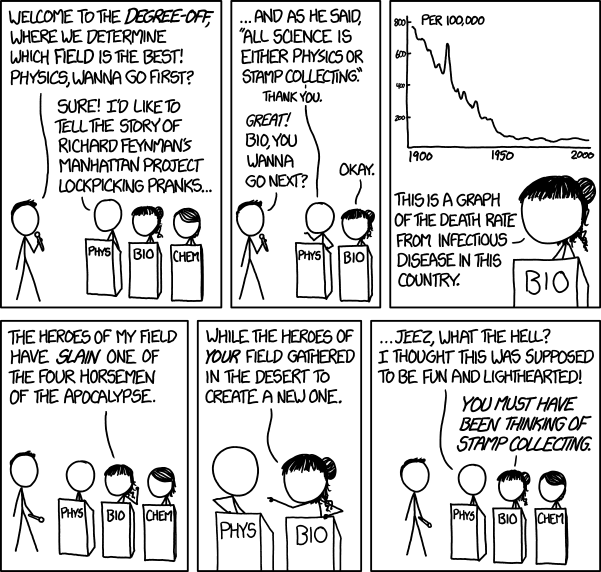
\includegraphics{./images/xkcd-disease-eradication.png}
\caption{Infectious disease control is arguably one of the greatest
successes of epidemiology and biology.}
\end{figure}

\section{Exercises}\label{exercises-8}

\begin{itemize}
\tightlist
\item
  The \emph{ID Control} app in the DSAIDE package provides hands-on
  computer exercises for this chapter.
\item
  Read the article ``Towards the endgame and beyond: complexities and
  challenges for the elimination of infectious diseases'' by Klepac et
  al. (Klepac et al. \protect\hyperlink{ref-klepac13}{2013}). Choose
  some ID - either one listed in box 1 of the paper or a different one -
  and discuss the current plans for elimination/eradication. What
  features of the ID will likely be helpful or unhelpful with regard to
  eradication/elimination? Reference the different areas the paper
  discusses? What is your overall assessment of feasibility?
\end{itemize}

\section{Further Resources}\label{further-resources-8}

\begin{itemize}
\tightlist
\item
  The relatively new Dengue vaccine raises interesting questions
  regarding the interplay of vaccination coverage and disease severity
  and is analyzed for instance in (Ferguson et al.
  \protect\hyperlink{ref-ferguson16}{2016}).
\item
  A brief discussion of ID control is provided in (Halloran and Longini
  \protect\hyperlink{ref-halloran14}{2014}).
\end{itemize}

\section{References}\label{references-9}

\chapter{Infectious Disease
Surveillance}\label{infectious-disease-surveillance}

\section{Overview and Learning
Objectives}\label{overview-and-learning-objectives-9}

In this module, we will take a look at surveillance of different
infectious diseases.

The learning objectives for this chapter are:

\begin{itemize}
\tightlist
\item
  Understand surveillance
\end{itemize}

\section{Introduction}\label{introduction-9}

To be able to implement successful interventions, we first need to know
what is actually happening. Once we implemented a control strategy, we
also want to know how it works. For both of those goals, good
surveillance is key.

\section{Goals of Surveillance}\label{goals-of-surveillance}

\begin{itemize}
\tightlist
\item
  Identify new emerging diseases as quickly as possible
\end{itemize}

\section{Types of Surveillance}\label{types-of-surveillance}

Active and passive

Medical/clinical and sequence

Ongoing or ad-hoc

\section{Problems with surveillance}\label{problems-with-surveillance}

Knowing numerator and denominator. Bias due to getting more severe
cases. Behavior change during an outbreak.

\section{Summary and Cartoon}\label{summary-and-cartoon-9}

\begin{figure}
\centering
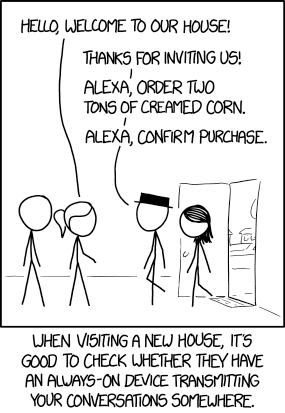
\includegraphics{./images/xkcd-listening.png}
\caption{A comprehensive, `always on' surveillance for infectious
diseases would be ideal.}
\end{figure}

\section{Exercises}\label{exercises-9}

\begin{itemize}
\item
\end{itemize}

\section{Further Resources}\label{further-resources-9}

\begin{itemize}
\item
\end{itemize}

\section{References}\label{references-10}

\chapter{Host Heterogeneity}\label{host-heterogeneity}

\section{Overview and Learning
Objectives}\label{overview-and-learning-objectives-10}

In this module, we will briefly discuss the idea that hosts differ in
characteristics that are important with regard to ID dynamics and
control.

The learning objectives for this chapter are:

\begin{itemize}
\tightlist
\item
  Know the most common host characteristics that lead to heterogeneity
\item
  Understand how heterogeneity might impact ID dynamics
\item
  Evaluate the need to account for heterogeneity depending on setting
\item
  Understand how different types of heterogeneity affect ID control
\end{itemize}

\section{Introduction}\label{introduction-10}

So far, we tracked hosts concerning their infection status (susceptible,
infected, symptomatic, recovered, etc.). We assumed that hosts are
similar enough with regard to any other characteristics that might
matter for ID dynamics and control that we did not have to consider
them. For instance, we did not account for age, sex, pre-existing
conditions or any other such potentially differentiating detail among
hosts.

That approach is of course at best a decent approximation and at worst
completely wrong. Many characteristics affect how an ID interacts with a
host. For instance, for many ID, children and the elderly are more
likely to get infected and might suffer more severe symptoms. For other
ID, only specific groups are affected. For instance, only sexually
active individuals are at risk of contracting a sexually transmitted
infection (ignoring for a moment less common transmission routes such as
blood transfusion for HIV). We will discuss some of these
differences/heterogeneities between hosts and how they affect ID
transmission and control in this module.

\section{Types of Host Heterogeneity}\label{types-of-host-heterogeneity}

We generally only care about differences in hosts as they relate to the
infectious disease process. Consider a simple - maybe silly - example:
Almost no infectious disease study (none that I know of) cares about a
person's hair color. That's because this characteristic has - as far as
we are aware - no effect on the interaction of host and ID. On the other
hand, a fundamental feature that affects many IDs is age. Therefore age
often needs to be taken into account when studying IDs. Other important
more broad categories such as genetics and behavior can also affect ID
infection and spread.

Some host characteristics might only have an impact on a single
component of the ID, e.g., the level of susceptibility to infection.
Other host differences can affect multiple components, e.g., a person
with numerous sexual partners is more likely to contract an STI, and if
they are infected, they are also more likely to transmit an STI.

\subsection{Host Heterogeneity Examples}\label{myexamplebox}

Several famous examples show how differences in genetics can impact ID.
For instance, persons with a certain mutation of the CCR5 co-receptor on
T-cells are much less likely to get infected with HIV. Similarly,
persons with a particular mutation in the FUT2 gene are much less likely
to get infected with norovirus. It is probable that there are genetic
differences for almost any ID that influence the probability of getting
infected, the severity of symptoms, and the duration and amount of
shedding.

\section{Heterogeneity in Transmission: Core
Groups}\label{heterogeneity-in-transmission-core-groups}

To study ID transmission dynamics, differences in the potential and
ability of individual hosts to spread an ID are obviously of great
importance. This idea of heterogeneity in transmission has been studied
in several contexts and under different names. One of the first was the
concept of a core group introduced to explain the persistence of
gonorrhea in the 1970s (see (Yorke, Hethcote, and Nold
\protect\hyperlink{ref-yorke78}{1978})). Core groups are subgroups in
which transmission is higher compared to other groups. For many STI,
transmission in the general population is low enough that the
reproductive number is below 1. The question then is, why does that not
lead to the extinction of the ID? The core group concept provides a
reasonable explanation. Where a small but defined population of
individuals maintain the ID with a reproductive number that is greater
than 1. Infections spread from this group to those in the general
population allows the ID to persist in the general population with a
reproductive number less than 1.

Once we have identified that different groups have different
transmission behavior, it also becomes necessary to understand how
individuals belonging to one of the groups interact with people of the
other groups. Often called the \emph{mixing} pattern between groups. We
are most interested in the mixing and contact patterns that facilitate
transmission of the ID under consideration. For instance, it is well
known that humans tend to have more contacts with others of the same
age, e.g., children predominantly contacting other children. This is
called \emph{assortative} mixing, and such age-specific mixing is
important for the transmission of many respiratory diseases. The
opposite is \emph{disassortative} mixing. For instance, for STI, most
mixing occurs between individuals from the opposite sex (and there are
also more contacts among individuals of similar age). Therefore, for
STI, mixing with regard to gender can be considered
\emph{disassortative}. However, it is also known that people who engage
in risky sexual behavior (e.g., more partners per year) tend to have
more contacts with others that engage in similar risk behavior, thus
with regard to transmission and infection risk, STI often show
\emph{assortative} mixing. If there is no mixing preference, it is
called \emph{random} mixing. The \emph{random} mixing assumption is made
implicitly in any model that does not account for contact/transmission
heterogeneity, e.g., the basic SIR model assumes \emph{random} mixing
and contact patterns between susceptible and infected, independent of
any other characteristic. Determining the mixing patterns between
individuals is important but also difficult. For some research in that
area, see, e.g. (Edmunds et al. \protect\hyperlink{ref-edmunds06}{2006};
Mossong et al. \protect\hyperlink{ref-mossong08}{2008}).

\section{Heterogeneity in Transmission:
Superspreaders}\label{heterogeneity-in-transmission-superspreaders}

An equivalent concept to that of the core group, but applied to
individuals, is known by the term superspreaders. Superspreaders are
individuals who spread/transmit an ID much more than the \emph{average}
infected person. It turns out that for most ID, the number of secondary
transmissions produced by the average infected person is not too
meaningful. Such a measure would be a good description if the
distribution of secondary infections were close to normal (or Poisson),
with most infected individuals infecting similar numbers of others.
However, what is often observed is a heavily skewed distribution, with
most individuals infecting none or only a few others, and a few
individuals infecting many others (Galvani and May
\protect\hyperlink{ref-galvani05}{2005}).

\section{Heterogeneity and The Reproductive
Number}\label{heterogeneity-and-the-reproductive-number}

If we have multiple host types, we need to extend the idea of the
reproductive number. While it is possible to compute a reproductive
number for the overall population, this quantity might not tell the full
story. Instead, we might want to look at the reproductive number for
subsets of the population, for instance for the general population
(non-superspreaders) and core groups (the superspreaders). If one wants
to compute an overall reproductive number, one needs to account for the
population heterogeneity by including a measure of the variability of
contacts in the equation for the reproductive number. See, (May, Gupta,
and McLean \protect\hyperlink{ref-may01}{2001}) for a discussion of this
topic.

\section{Heterogeneity and ID
control}\label{heterogeneity-and-id-control}

Heterogeneity among hosts concerning their susceptibility,
infectiousness, and severity has direct implications for control. If we
know who is most likely to transmit, who is most likely to have a severe
case of a disease, and who is most likely to catch an ID in the first
place, we can implement targeted control strategies. For instance,
instead of vaccinating people at random, we could target those that are
most vulnerable to getting the ID, or those most likely to infect others
if they were to get infected. The better we can target the intervention,
the more impact they can have, and while also getting more `bang for our
buck'.

\section{Modeling Heterogeneity}\label{modeling-heterogeneity}

The basic concept of including host heterogeneity in models is
relatively straightforward. We stratify the population according to the
characteristic we want to take into account. For instance, instead of
lumping everyone into susceptible-infected-recovered categories, we can
track males and females, or children and adults, separately. Figure
\ref{fig:heterogeneity} illustrates this.

\begin{figure}
\centering
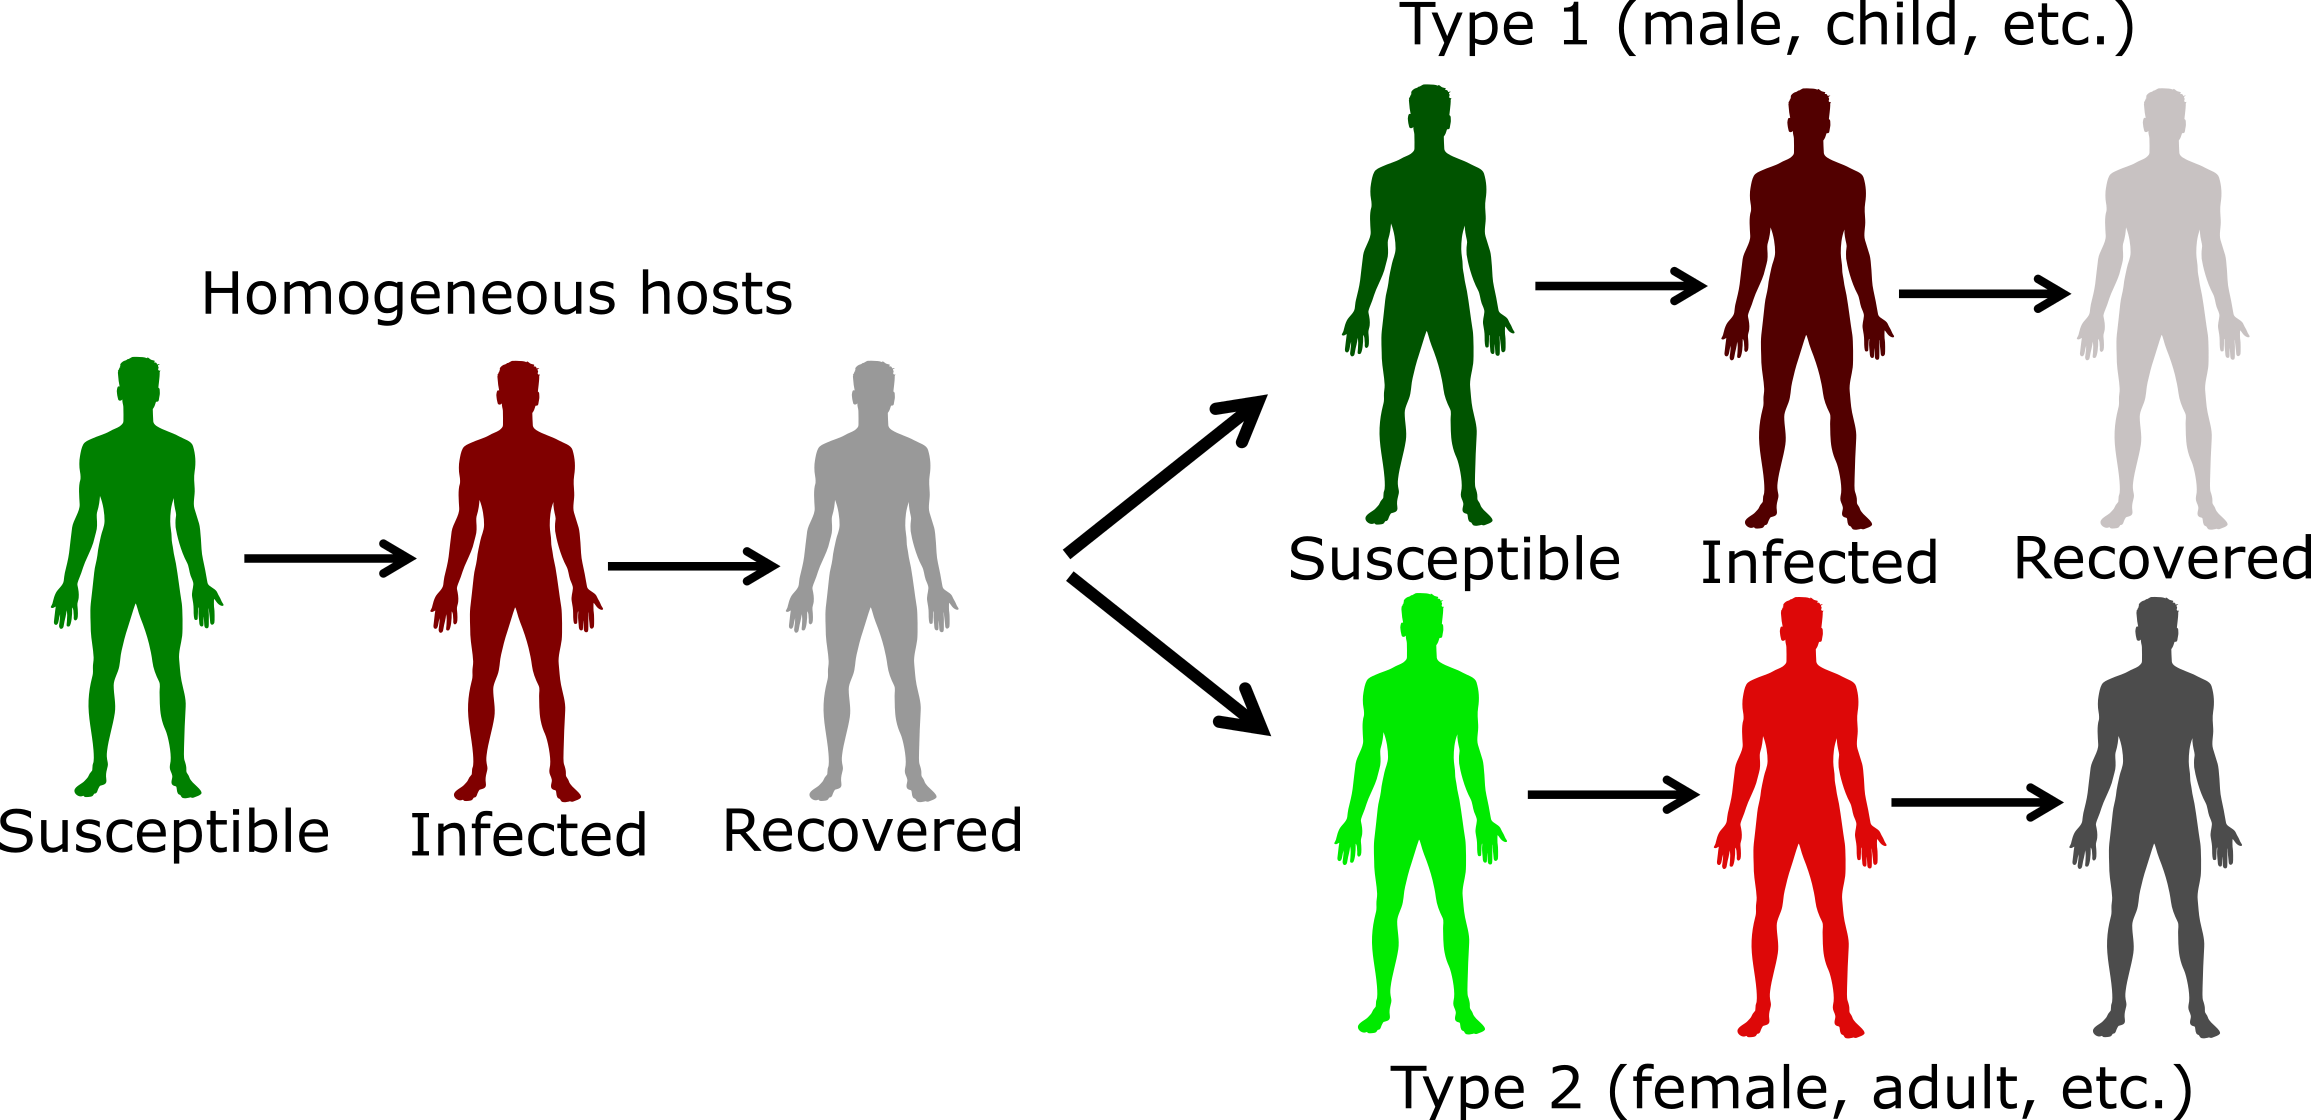
\includegraphics{./images/heterogeneityexample.png}
\caption{\label{fig:heterogeneity}Example of including host heterogeneity in
an SIR model.}
\end{figure}

The challenges with including more details in the model are not
conceptual but are instead logistical and potentially technical. Bigger
models are harder to formulate, implement, and analyze. Additionally, we
need estimates of model parameters with regard to the stratifying
characteristics, which are often hard to get. Because of that, it is
often best to start with a simple model, and slowly introduce host
characteristics as they are deemed relevant to the ID setting, and
question one wants to address.

At some point, if we want to include a lot of detail, it might be worth
switching the modeling framework. For compartmental models, hosts are
grouped according to characteristics. As we want to track more
characteristics, the number of compartments we need to include
increases. If the basic model has C compartments/variables, P
parameters, and we model N subpopulations, we have C x N equations and
at least P x N (or more) parameters. For instance, if we had a basic
SEIR model (4 compartments), and wanted to track males and females in 4
different age groups, we had 4 x 2 x 4 = 32 compartments. If we had
additional compartments to follow say vaccination or treatment status,
one could end up with more than 50 compartments, sometimes even going
into the hundreds.

Once the number of compartments gets too large, it might then be worth
deciding to stop using compartmental models and instead switch to a type
of model that is called agent or individual-based model (ABM/IBM). In
such models, the individual host is modeled and tracked. We can give
everyone as many different characteristics as we want. This makes the
model very flexible and potentially very realistic. The downside of
these ABM is that they tend to be more complicated than compartmental
models, are generally much harder to code, and often take a long time to
run, especially if one wants to model a large population. Further, for
detailed models, lots of parameter estimates are needed, and they are
often not available, leading to potentially large uncertainty in model
predictions. Also, it 's hard to make any statistical inference with
ABM. Because of these disadvantages, the compartmental modeling
framework is still the most frequently used and a good starting point
for most situations and questions. For IDs where we know a lot and want
detailed predictions (e.g., influenza), ABMs are becoming more common.

\section{Summary and Cartoon}\label{summary-and-cartoon-10}

This chapter provided a brief discussion of host heterogeneity, how to
consider it in studies, and its impact on transmission and control. We
also discussed how to include heterogeneity into models.

\begin{figure}
\centering
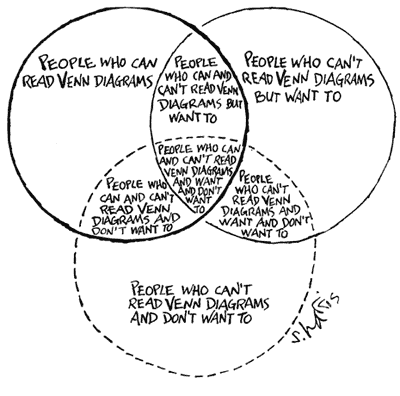
\includegraphics{./images/crazyvenndiagram.png}
\caption{\label{fig:crazyvenndiagram}That is the best heterogeneity cartoon
I have - let me know if you know a better one!}
\end{figure}

\section{Exercises}\label{exercises-10}

\begin{itemize}
\tightlist
\item
  The \emph{Host Heterogeneity} app in the DSAIDE package provides
  hands-on computer exercises for this chapter.
\item
  Read the article ``Disease spread, susceptibility, and infection
  intensity: vicious circles?'' by Beldomenico and Begon (Beldomenico et
  al. \protect\hyperlink{ref-beldomenico09}{2009}). The paper mostly
  discusses non-human IDs. Find evidence from human IDs for which the
  different components they discuss (variable host susceptibility,
  variable infection intensity, feedback circles in the
  individual/population level) might be applicable.
\end{itemize}

\section{Further Resources}\label{further-resources-10}

\begin{itemize}
\tightlist
\item
  Good further discussions of the superspreader concept can be found in
  (Galvani and May \protect\hyperlink{ref-galvani05}{2005}; Lloyd-Smith
  et al. \protect\hyperlink{ref-lloyd-smith05}{2005}; Stein
  \protect\hyperlink{ref-stein11}{2011}).
\item
  The impact of host heterogeneity on the reproductive number is for
  instance discussed in (May, Gupta, and McLean
  \protect\hyperlink{ref-may01}{2001}), an application to Chlamydia is
  provided in (Potterat et al.
  \protect\hyperlink{ref-potterat99}{1999}).
\item
  An influential study that collected detailed information on contact
  patterns using a diary approach is (Mossong et al.
  \protect\hyperlink{ref-mossong08}{2008}).
\item
  General discussions of transmission heterogeneity are given in
  (Matthews and Woolhouse \protect\hyperlink{ref-matthews05}{2005};
  Paull et al. \protect\hyperlink{ref-paull12}{2012}).
\item
  Host heterogeneity and control is for instance discussed in (Yorke,
  Hethcote, and Nold \protect\hyperlink{ref-yorke78}{1978}; Woolhouse et
  al. \protect\hyperlink{ref-woolhouse97}{1997}).
\end{itemize}

\section{References}\label{references-11}

\chapter{Dynamics of Multiple
Pathogens}\label{dynamics-of-multiple-pathogens}

\section{Overview and Learning
Objectives}\label{overview-and-learning-objectives-11}

In this chapter, we will discuss scenarios where more than one
infectious disease is considered simultaneously.

The learning objectives for this chapter are:

\begin{itemize}
\tightlist
\item
  Know important multi-ID systems
\item
  Understand how IDs can interact
\end{itemize}

\section{Introduction}\label{introduction-11}

So far, we focused on a single ID at a time. The main reason for this is
simplicity. A single ID is already difficult to study and leads to
complex dynamics. It makes sense to first study and understand
individual IDs before including further IDs. That said, there are always
many pathogens present at the same time, and infection with more than
one ID is very common (Petney and Andrews
\protect\hyperlink{ref-petney98}{1998}). This is true in the developed
world with a fairly low ID burden, and even more so in developing
countries. It is thus often useful to consider systems with more than
one ID.

\section{Interactions of ID}\label{interactions-of-id}

Sometimes, different IDs do not interact, i.e., being infected with one
does not impact the susceptibility or course of infection for another
ID. It is likely that some amount of interaction occurs for almost all
IDs, mediated by the immune response or through other mechanisms such as
a change in host behavior or host death (Rohani et al.
\protect\hyperlink{ref-rohani03}{2003}). However, unless the IDs are
relatively common and the interaction effect is strong, it is often hard
to determine if and how IDs affect each other. As such, we know how some
IDs interact (e.g., TB and HIV) but for most ID, we have very little
knowledge. The next few sections briefly discuss some IDs for which we
have some understanding regarding interactions. This is not an
exhaustive discussion. Instead, we focus on some of the best-known
interactions.

\subsection{HIV-TB Interactions}\label{hiv-tb-interactions}

HIV is the pathogen that is best studied with regard to interaction with
other pathogens (Karp and Auwaerter
\protect\hyperlink{ref-karp07}{2007}\protect\hyperlink{ref-karp07}{b};
Karp and Auwaerter
\protect\hyperlink{ref-karp07a}{2007}\protect\hyperlink{ref-karp07a}{a};
Griffiths et al. \protect\hyperlink{ref-griffiths11}{2011}). Arguably of
most public health interest and concern is the interaction with TB.
Having an (untreated) HIV infection makes it much more likely for an
individual latently infected with TB to develop TB disease. Further,
once TB disease develops, an individual who is also infected with HIV
has worse symptoms and a much higher chance of dying (Pawlowski et al.
\protect\hyperlink{ref-pawlowski12}{2012}). An important current
question that is still not fully answered is if the suppression of HIV
by antiretroviral therapy treatment removes all detrimental effects of
HIV on TB progression, or if the presence of HIV, albeit at minuscule
levels, still has a negative impact on TB disease progression.

\subsection{HIV-Hepatitis
Interactions}\label{hiv-hepatitis-interactions}

Persons infected with HIV are also often at risk of having HBV or HCV
infections. The primary reason for this is that risk factors for these
pathogens are very similar (e.g., drug use) (Sulkowski
\protect\hyperlink{ref-sulkowski08}{2008}). Co-infection leads to faster
rate of liver failure (Chen, Feeney, and Chung
\protect\hyperlink{ref-chen14}{2014}). If HBV or HCV leads to more rapid
progression to AIDS and HIV-mediated death is unclear (Kim and Chung
\protect\hyperlink{ref-kim09}{2009}). It seems that with antiretroviral
therapy and the new drugs against viral hepatitis, the impact of this
co-infection on health can be minimized.

\subsection{Influenza-Strep
Interactions}\label{influenza-strep-interactions}

The interaction of influenza with some bacteria and most notably
\emph{Streptococcus pneumoniae} has been somewhat well studied
(McCullers \protect\hyperlink{ref-mccullers06}{2006}). Some careful
animal experiments, as well as modeling studies, have shown how
influenza interacts with bacteria co-infections (Smith and McCullers
\protect\hyperlink{ref-smith14a}{2014}; Shrestha et al.
\protect\hyperlink{ref-shrestha13}{2013}). In general, an influenza
infection seems to make it more likely - during a short time window - to
have a subsequent bacterial infection, and the outcome of the bacterial
infection is often worse. It is still not well understood if there is
also an effect of a respiratory bacterial infection on a potential
secondary influenza infection (Davis et al.
\protect\hyperlink{ref-davis12}{2012}).

\section{More Than Two Infectious
Diseases}\label{more-than-two-infectious-diseases}

While not much is known about interactions between any two ID (apart
from the examples just described and a few others), even less is known
for 2+ ID. It is fair to say that given our current level of knowledge
about the biology and epidemiology of various ID, understanding
interactions and dynamics of multiple ID is beyond our current scope,
and will likely remain so for a while.

\section{Multiple ID and Control}\label{multiple-id-and-control}

If multiple IDs are present, it makes sense to try and implement control
strategies against as many of them as possible. This is true for
diseases which interact or are independent. Unfortunately, given the way
health systems are structured and funded, it is still often the case
that interventions target a single ID at a time. E.g., a campaign
against malaria focuses solely on malaria treatment, even though many of
the patients probably also have TB or some helminth infections and
should be tested and treated for those diseases at the same time. The
one important exception is HIV. Often HIV testing and treatment is
included even if a study or health campaign focuses on a different
disease. Having a more wide-spread multi-ID approach to control would
very likely be highly effective since, for many ID, individuals who are
likely to get infected with one are also likely to get infected with
other ID. This is because many IDs have the same risk factors for
transmission from poor nutrition or unsanitary conditions to particular
behaviors that increase the risk for multiple IDs. One could, therefore,
efficiently find and effectively treat many different IDs. Public health
is slowly moving this direction.

Some ways in which multiple IDs are controlled are almost accidental. It
is well known that better education, better nutrition, better standard
of living, improved sanitation and housing all reduce morbidity and
mortality to a large number of diseases. As developing countries become
richer and people escape extreme poverty, the incidence of many IDs
fall. This is the trajectory many developed countries were on, e.g., TB
incidence in Europe was falling rapidly even before the introduction of
anti-TB drugs. As more countries become developed, the ID burden will
decline (and likely with it, ``wealth diseases'' like obesity will
rise).

\section{Modeling multiple ID}\label{myadvancedbox}

The approach to modeling multiple ID is similar to that of host
heterogeneity: We need to split/stratify the population according to
infection status of each ID. The complicated part is modeling any
potential interactions between IDs correctly. As mentioned previously,
more compartments the more complex the model becomes. Making it harder
to code, analyze, and we need estimates for each parameter, which are
often hard to get. Because of that, considering/modeling more than 2 ID
is still almost never done - but many critical 2-ID modeling studies
exist. Figure \ref{fig:coinfection} shows the diagram for a 2 ID model.

\begin{figure}
\centering
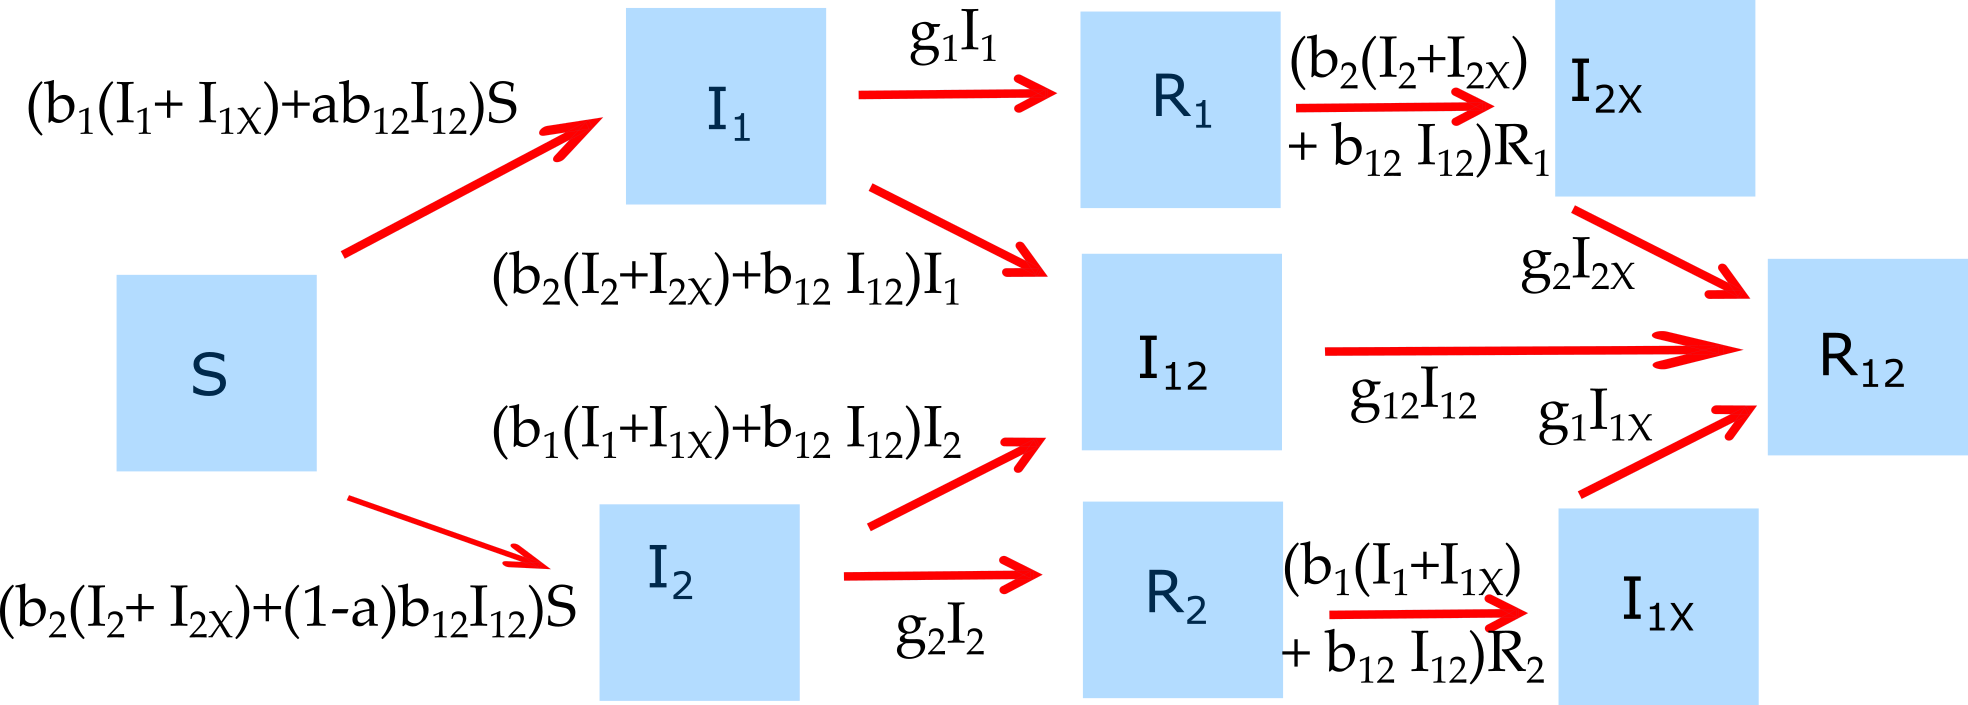
\includegraphics{./images/multipathogenmodel.png}
\caption{\label{fig:coinfection}Example of a model that considers 2 ID.}
\end{figure}

The differential equations corresponding to this diagram are given by:

\[\dot S =  -  (b_{1} (I_1+I_{1X}) + b_{2} (I_2+I_{2X}) + b_{12}I_{12}) S  \]
\[\dot I_1 =   (b_{1} (I_1+I_{1X}) + ab_{12} I_{12})S - (g_1  + b_{2} (I_2+I_{2X})  + b_{12}  I_{12}) I_1\]
\[\dot I_2 =   (b_{2} (I_2+I_{2X}) +  (1-a) b_{12} I_{12})S - (g_2 + b_{1}(I_1 + I_{1X}) + b_{12} I_{12}) I_2\]
\[\dot I_{12} = (b_{2} (I_2+I_{2X})  + b_{12}  I_{12}) I_1 + (b_{1}(I_1 + I_{1X}) + b_{12} I_{12}) I_2  - g_{12} I_{12}\]
\[\dot R_1 = g_1 I_1 - (b_2 (I_2 + I_{2X}) + b_{12}  I_{12}) R_1\]
\[\dot R_2 = g_2 I_2 - (b_1 (I_1 + I_{1X}) + b_{12}  I_{12}) R_2\]
\[\dot I_{1X} = (b_1 (I_1 + I_{1X}) + b_{12}  I_{12}) R_2 - g_{1} I_{1X}\]
\[\dot I_{2X} = (b_2 (I_2 + I_{2X}) + b_{12}  I_{12}) R_1 - g_{2} I_{2X}\]
\[\dot R_{12} = g_{1} I_{1X} + g_{2} I_{2X} + g_{12} I_{12} \]

\section{Summary and Cartoon}\label{summary-and-cartoon-11}

This chapter discussed multi-pathogen systems.

\begin{figure}
\centering
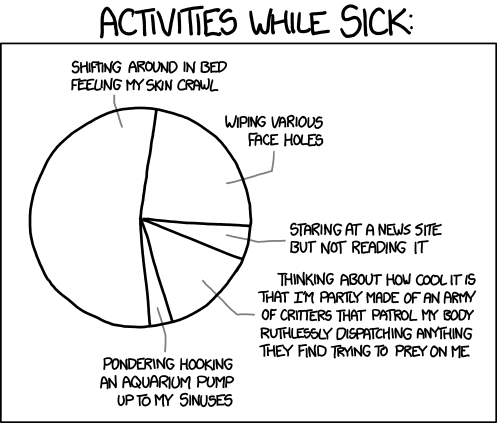
\includegraphics{./images/xkcd-sick_day.png}
\caption{I don't have a topical cartoon, so instead just a random one.
Let me know if you find a suitable one!}
\end{figure}

\section{Exercises}\label{exercises-11}

\begin{itemize}
\tightlist
\item
  The \emph{Multi-pathogen dynamics} app in the DSAIDE package provides
  hands-on computer exercises for this chapter.
\item
  Read the article ``The nature and consequences of coinfection in
  humans'' by Griffiths et al. (Griffiths et al.
  \protect\hyperlink{ref-griffiths11}{2011}). They report that for
  several of the ``top 10'' ID no co-infection studies could be found
  among 2009 publications. See if you can find any coinfection studies
  on one of those IDs that were published since. Describe and summarize
  the studies you found.
\end{itemize}

\section{Further Resources}\label{further-resources-11}

\begin{itemize}
\tightlist
\item
  The references mentioned in this chapter provide further information
  on specific topics.
\item
  An interesting modeling study looking at potential interactions of HIV
  and Malaria is (Abu-Raddad, Patnaik, and Kublin
  \protect\hyperlink{ref-abu-raddad06}{2006}).
\item
  A review of possible interactions between TB and parasitic infections
  can be found in (Li and Zhou \protect\hyperlink{ref-li13}{2013}).
\item
  A very nice analysis of the impact of measles and measles vaccination
  on other childhood infectious diseases is given in (Mina et al.
  \protect\hyperlink{ref-mina15}{2015}).
\end{itemize}

\section{References}\label{references-12}

\chapter{Stochastic Dynamics and
Extinctions}\label{stochastic-dynamics-and-extinctions}

\section{Overview and Learning
Objectives}\label{overview-and-learning-objectives-12}

In this chapter, we take a look at stochasticity and how it impacts ID
dynamics. A focus is on the potential of ID extinction. We discuss how
one needs to account for stochasticity in models if one wants to study
extinction.

The learning objectives for this chapter are:

\begin{itemize}
\tightlist
\item
  Understand the difference between stochastic and deterministic models
\item
  Know when one needs to make use of stochastic models
\item
  Understand the concept of critical community size
\item
  Understand how stochasticity affects ID dynamics and can lead to
  extinctions
\end{itemize}

\section{Deterministic Models}\label{deterministic-models}

So far, all the models we have used to explore different aspects of ID
dynamics have been \emph{deterministic}. For a deterministic model, once
you choose the initial conditions and parameter values, you always get
the same result, no matter how often you run the model. There is no
randomness present.

Such deterministic models are relatively easy to implement and to study.
That is one of the reasons they are so commonly used. Such a modeling
approach also often provides a good representation of the dynamics of
real ID if numbers are large. That is due to the law of large numbers.
While every individual host or pathogen undergoes somewhat random
dynamics, these random parts get \emph{averaged out}, and the dynamics
of the whole population is fairly predictable and well described by such
deterministic models. (This is the same concept we use in classical
epidemiological studies, where we enroll sufficiently large numbers such
that we can say something predictable about differences between groups,
even if individuals are somewhat unpredictable.)

\section{Stochasticity}\label{stochasticity}

Biological systems are never deterministic. When numbers are small,
randomness starts to matter. As an example, consider an outbreak of some
ID. Let's say we have a group of 100 infected. At a given time, some of
them will transmit to others, and after that, they will recover from the
disease, while others will recover before infecting others. The overall
outbreak dynamics can be well approximated by a deterministic model if
we accurately specify the average rate of transmission and the average
rate of recovery. In contrast, now assume that there is a single
infected person. Now it makes a huge difference if this person transmits
to someone else before recovering, or if they recover before
transmission occurs. In the latter case, the outbreak is over, and the
ID has gone extinct. Thus, at small numbers, randomness/unpredictability
in the order of events can make a large difference.

\section{Discrete Numbers and
Extinctions}\label{discrete-numbers-and-extinctions}

Another problem inherent in the deterministic differential equation
based models we have looked at so far is that they treat individuals in
each compartment as continuous. For instance, the models allow 142.7
infected hosts. Of course, in reality, those numbers have to be
integers. If we are dealing with large numbers, the difference between
142.7 and 142 or 143 is minor and doesn't matter. However, once numbers
get small, the fact that we are dealing with discrete numbers of hosts
becomes significant. So once less than 1 host has an infection the ID is
in reality gone, but a continuous model would instead allow the number
of infected to drop below 1 but remain above 0. In this way, the ID in
the continuous models never actually goes extinct, it only gets closer
and closer to 0 (and at some point is so close to 0 that the computer
can't distinguish it from 0 anymore).

\section{Modeling Stochasticity and
Extinction}\label{modeling-stochasticity-and-extinction}

To capture both the randomness and discrete nature of real systems
requires a slightly different modeling approach. We can still use
compartmental models, i.e., we track total numbers of individuals in
particular states (e.g., S-I-R). But now, instead of letting the numbers
in each compartment change continuously through inflows and outflows,
changes happen in discrete steps, determined by specific events that
occur in a probabilistic manner.

As an example, instead of new susceptible hosts entering the system at
some continuous birth rate, we now model births occurring as discrete
events. Each birth event leads to an increase in the number of
susceptibles by 1. The timing of the birth events is somewhat random,
with an overall probability determined by the model (e.g., a higher
birth rate will mean births occur more frequently, but still randomly).

\section{Factors Affecting
Extinction}\label{factors-affecting-extinction}

Extinction of ID is of interest because that is often our final goal. We
would like to drive an ID to extinction, either locally or even better,
globally. If and how an ID can be driven to extinction depends on
different factors. For IDs in humans, the only real chance is to tackle
those with no other hosts or reservoirs. As such, we will likely never
be able to eradicate influenza. But measles eradication might be
possible (though hard).

Factors related to the host population and distinct ID characteristics
influence the likelihood of an ID to go extinct. Two significant
population factors are the size of the host population and the speed at
which new susceptible hosts are replenished. Important characteristics
of the ID included the infectiousness, the duration of the latent and
infectious periods, the ability of the ID to persist outside the host,
and other.

\section{Critical Community Size}\label{critical-community-size}

The minimum size of a population at which an ID can maintain itself in a
population without extinction has been termed the Critical Community
Size (CCS) (this also depends on the replenishment of new susceptibles,
e.g., birth rates). Studies for measles suggested that the CCS was
several hundred thousand (Keeling and Grenfell
\protect\hyperlink{ref-keeling02}{2002}), meaning that measles could
have only become a human pathogen once human populations were large
enough to maintain it. The CCS is the number of susceptibles in a
population and does not include those who are immune. Through
vaccinating it is possible to reduce the size of the susceptible
population below the CCS. So it is not necessary to vaccinate everyone
to get an ID to go extinct. We just need to reach enough individuals to
get the population of susceptibles below the critical level. This task
is already hard by itself, as evidenced by the fact that we have not
been able to eradicate measles, despite having a good vaccine.

\section{Host Extinction}\label{host-extinction}

Another way an ID can go extinct is if its hosts go extinct - either due
to mortality from the ID or other causes. For most human diseases, such
host extinction is fortunately not very common - though highly lethal ID
such as Ebola can lead to marked reduction in the number of hosts in a
given population. For non-human disease, extinctions of hosts due to
disease is a more significant issue. Here, conversation efforts might
try to achieve non-extinction of the host and - ideally - extinction of
the ID.

The host extinction approach is also often considered and used for
vector-borne diseases. Here, the idea is to drive one of the hosts
(commonly called the vector) to extinction. The obvious reasoning is
that if there are fewer vectors (e.g., mosquitoes), the chances for
humans to get infected are lower. Widespread use of DDT or
insecticide-coated bed-nets are examples of this. A similar but more
controversial approach is the attempted control of rabies in humans by
killing its primary host, vampire-bats (Stoner-Duncan, Streicker, and
Tedeschi \protect\hyperlink{ref-stoner-duncan14}{2014}).

\section{Disease Emergence}\label{disease-emergence}

The flip-side of extinction is the emergence of a new disease. During
extinction, infected/pathogen numbers move from a level that can be
decently approximated by a deterministic model to numbers so small that
it requires a stochastic analysis approach to allow the possibility of
extinction. During emergence, the new disease starts at zero, then is
introduced in modest numbers (possibly only a single introduction) into
a new population, and ``bounces around'' for a while in small numbers.
If conditions are right (i.e., local reproductive number greater than
1), the disease might take off and spread (Antia et al.
\protect\hyperlink{ref-antia03}{2003}). It might eventually reach high
enough numbers that a deterministic approximation which focuses on the
mean dynamics is warranted. Many recent emerging disease outbreak
followed that pattern. The 2014 Ebola outbreak and 2009 Influenza
pandemic reached sufficiently large numbers that a deterministic
approach was reasonable, while the 2013 SARS epidemic and previous Ebola
outbreaks lead to relatively few cases, so a stochastic modeling and
analysis approach is likely more appropriate.

The next chapter discusses the evolution and emergence of new diseases
in more detail, with a focus on drug resistance evolution and emergence.

\section{Summary and Cartoon}\label{summary-and-cartoon-12}

This module provides a brief discussion of stochasticity in ID dynamics,
and its relation to disease extinctions.

\begin{figure}
\centering
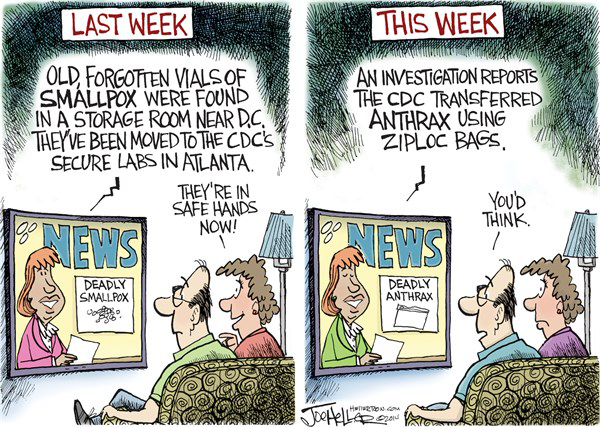
\includegraphics{./images/smallpox.png}
\caption{\label{fig:smallpox}Smallpox is \emph{almost} extinct.}
\end{figure}

\section{Exercises}\label{exercises-12}

\begin{itemize}
\tightlist
\item
  The \emph{Stochastic dynamics} app in the DSAIDE package provides
  hands-on computer exercises for this chapter.
\item
  Read the article ``Measles Endemicity in Insular Populations: Critical
  Community Size and Its Evolutionary Implication'' by Black (Black
  \protect\hyperlink{ref-black66}{1966}). The paper discusses critical
  community size for measles. Find 2 papers/analyses that discuss the
  CCS for other IDs. Read, summarize and critique the papers.
\end{itemize}

\section{Further Resources}\label{further-resources-12}

\begin{itemize}
\tightlist
\item
  Some further analysis of critical community size and measles can be
  found in (Bartlett \protect\hyperlink{ref-bartlett57}{1957}; Bartlett
  \protect\hyperlink{ref-bartlett60}{1960}; M J Keeling
  \protect\hyperlink{ref-keeling97}{1997}; M. J. Keeling
  \protect\hyperlink{ref-keeling97a}{1997}).
\item
  Some further discussion of stochastic epidemic models can be found in
  (Black and McKane \protect\hyperlink{ref-black12}{2012}; Britton
  \protect\hyperlink{ref-britton10a}{2010}).
\item
  A broad discussion of invasion and persistence of ID and the role of
  stochasticity is given in (J. O. Lloyd-Smith et al.
  \protect\hyperlink{ref-lloyd-smith05b}{2005}).
\item
  An interesting discussion of critical community size and its
  dependence on birth dynamics, especially birth pulses, is provided in
  (Peel et al. \protect\hyperlink{ref-peel14}{2014}).
\end{itemize}

\section{References}\label{references-13}

\chapter{Evolutionary Dynamics}\label{evolutionary-dynamics}

\section{Overview and Learning
Objectives}\label{overview-and-learning-objectives-13}

In this chapter, we will take a look at ID-evolution and its relation to
control measures.

The learning objectives for this chapter are:

\begin{itemize}
\tightlist
\item
  Understand the central mechanisms and drivers of ID-evolution
\item
  Be able to assess how different control strategies can affect
  ID-evolution
\end{itemize}

\section{Introduction}\label{introduction-12}

Evolution is based on the generation of diversity, usually genetic
diversity through mutations and the subsequent increase or decrease in
certain genetic variants through selection or random drift.
Microorganisms, especially viruses, tend to undergo rapid evolutionary
change. High mutation rates and large population sizes provide many
opportunities for the generation of genotypic and phenotypic diversity.
Short generation times and fluctuations in population size (e.g.,
through transmission bottlenecks) allow selection to quickly act on this
diversity, amplifying those mutants that have a fitness advantage and
eliminating those with low fitness. These features of microbial
populations often lead to rapid evolutionary changes. Such evolutionary
change can become a public health problem.

\section{Evolution and Immune Escape}\label{evolution-and-immune-escape}

A powerful driver of evolution is the host immune response. If an ID
induces a strong immune response which subsequently protects the host
from re-infection, a mutant of the ID which can partially escape the
host immunity and infect a host will have a large fitness advantage.
This is the process which drives the continuous evolution of influenza
in humans. It is likely also the driver for changes in many other
diseases, especially viruses. Why some pathogens do not seem to evolve
much to circumvent immune response (measles is a good example) is not
quite clear, though some studies have speculated on that topic (Frank
and Bush \protect\hyperlink{ref-frank07}{2007}; Lange and Ferguson
\protect\hyperlink{ref-lange09}{2009}).

\section{Public Health Interventions and
Evolution}\label{public-health-interventions-and-evolution}

Some of the most potent drivers of evolution are in fact public health
interventions that try to reduce the burden of an ID. The more powerful
the intervention (e.g., vaccines or drugs), the more evolutionary
pressure a pathogen faces and the more advantaged a pathogen variant
that is partially or entirely resistant to the intervention will be. The
following sections briefly discuss several drivers of public health
importance that influence the selective fitness of different genetic
variants and thereby drive ID-evolution.

\subsection{Evolution of Immunity or Vaccine
Escape}\label{evolution-of-immunity-or-vaccine-escape}

Vaccines are some of our most potent interventions. Vaccination induces
immunity in the vaccinated hosts. If a pathogen can circumvent immunity
and infected vaccinated individuals, it will have a large fitness
advantage. Therefore, any mutation that arises which allows a pathogen
to reduce the impact of host immunity will likely spread through a
population quickly. Most immunity works through antibodies. Thus
pathogen variants that evolve not to be (or less) recognized by
pre-existing antibodies have an advantage. This is the same mechanism
induced by natural immunity. Thus, pathogens that frequently evolve to
escape natural antibody-based immunity (e.g., influenza, HIV) are also
able to develop resistance to vaccine-induced immunity. This is the
reason we need to get re-immunized with influenza vaccines regularly and
why we have not managed to develop an HIV vaccine. In contrast, an ID
like measles which does not seem to be able to escape natural immunity
also does not evolve resistance to the vaccine, and we can use the same
vaccine against measles we have been using for decades.

The reason why measles might not be able to escape binding by
pre-existing antibodies is likely because the binding site is also the
part of the virus that is needed to attach to and enter host cells. Any
mutation evading antibody binding would also lead to an inability to
attach to and infect cells. In contrast, for influenza, the antibody
binding regions and the receptor attachment regions are somewhat
distinct.

\subsection{Evolution of Drug
Resistance}\label{evolution-of-drug-resistance}

Drugs are another mechanism that applies a strong selective pressure.
Any pathogen that can avoid being killed by a drug can potentially `take
over' a patient and transmit to the next. If drug use is widespread in
the population, those resistant mutants which generally have lower
fitness than the wild-type, drug-sensitive strain can take over in a
population. This phenomenon has been observed with many different ID and
drugs and produced such looming public health problems as extensively
drug-resistant TB (XDR TB) and methicillin-resistant Staphylococcus
aureus (MRSA) (Levy and Marshall \protect\hyperlink{ref-levy04}{2004}).
Since viruses tend to evolve faster than bacteria, drug resistance
evolution is often a problem at the individual patient level. HIV is the
prime example. Single-drug therapy for HIV fails consistently because
the virus quickly evolved resistance. Only once we started using
multiple drugs at the same time were we able to prevent rapid evolution.
We are playing a `numbers game' since the chance of 3 resistance
mutations against 3 different drugs occurring is so small that it rarely
happens during the treatment of an individual host, thus making the
drugs effective for the host's lifetime. Since drug resistance is such
an important public health problem, it is widely studied. This includes
many modeling studies. For an overview of some of those, see (Louz et
al. \protect\hyperlink{ref-louz10}{2010}; Temime et al.
\protect\hyperlink{ref-temime08}{2008}; Wiesch et al.
\protect\hyperlink{ref-wiesch11}{2011}).

\section{Evolution of Virulence}\label{evolution-of-virulence}

The term virulence is a bit fuzzy, but it generally means `harm to the
host'. That could be due to mortality caused by an ID, or in less severe
forms, ID-related morbidity (sickness/symptoms). Pathogens `don't care'
about harming their hosts, their primary `purpose' is to get in,
replicate, and get back out and infect the next host. Sometimes,
inducing some morbidity in the host is useful for the pathogen. Sneezing
and coughing for respiratory infections might lead to enhanced
transmission and therefore increased pathogen fitness. In other
situations, inducing morbidity/mortality doesn't increase pathogen
fitness, but it also doesn't decrease it. Therefore, selection doesn't
act to change the number of symptoms induced. Pathogens that are too
virulent, and in extreme cases kill their hosts, generally have reduced
fitness since, in most situations, dead hosts do not transmit. The idea
is then that pathogens evolve to induce the level of virulence that is
optimal for their overall transmission fitness.

\section{Evolution and Public Health
Interventions}\label{evolution-and-public-health-interventions}

In general (apart from the possible phenomenon of drug-induced
hypermutation in bacteria), the generation of genetic variants is not
influenced by any human intervention. Those mutants are constantly
produced. In the usual setting, most mutants are less fit than the
wild-type strain and therefore are outcompeted. If not, they replace the
current strain and become the new wild-type. What happens in the
presence of interventions is that the fitness landscape changes. For
instance, if we give a patient drugs, a mutant resistant to drugs with a
fitness less than the wild-type in the absence of drug treatment has a
significant advantage and can outcompete the wild-type strain.

\section{Co-evolution}\label{co-evolution}

While the hosts infected by ID also evolve, this usually happens on much
slower time-scales. As such, studying evolution by assuming only the ID
evolves and not the host is often a good approximation. However, there
are examples where host evolution needs to be considered. A good example
is the introduction of myxoma virus to control Australian rabbit
populations. Evolution of both the virus and rabbits was observed. Over
longer time-scales, features such as sickle cell anemia, which comes
from a mutation that is associated with reduced malaria morbidity, is
likely a trait some humans evolved in response to malaria. A discussion
of genetic characteristics in humans that might be attributable to
evolution in response to specific infectious diseases is provided in
(Pittman et al. \protect\hyperlink{ref-pittman16}{2016}).

\section{Modeling Evolutionary
Dynamics}\label{modeling-evolutionary-dynamics}

To study evolutionary dynamics, we will need to implement models that
allow for changes in the system on top of the non-evolutionary dynamics
of the ID. Unless we plan to model many different potential new
variants, it is often easiest to pre-specify the number of variants we
want to track. In the simplest form where we only track pathogen
evolution, we might model the wild-type (normal, pre-existing) form of
the pathogen and a single mutant that is different in some important
characteristic, e.g., resistant to a drug or able to evade a vaccine. We
would build a model with these compartments. We often also pre-specify
the characteristics (i.e., the parameter values) for both the wild-type
and mutant. We implement the process of mutant generation in the model
and run the simulation. Under certain circumstances, we might see the
mutant be generated and take over the population.

If we want to model many different mutants, maybe allowing for random,
not pre-specified, differences in their fitness, and perhaps even
allowing for host evolution, the models get quite a bit more
complicated. They are not necessarily conceptually harder, but there is
more bookkeeping and coding involved making it technically trickier.

\section{Summary and Cartoon}\label{summary-and-cartoon-13}

This module provides a brief discussion of ID-evolution, especially
concerning ID control.

\begin{figure}
\centering
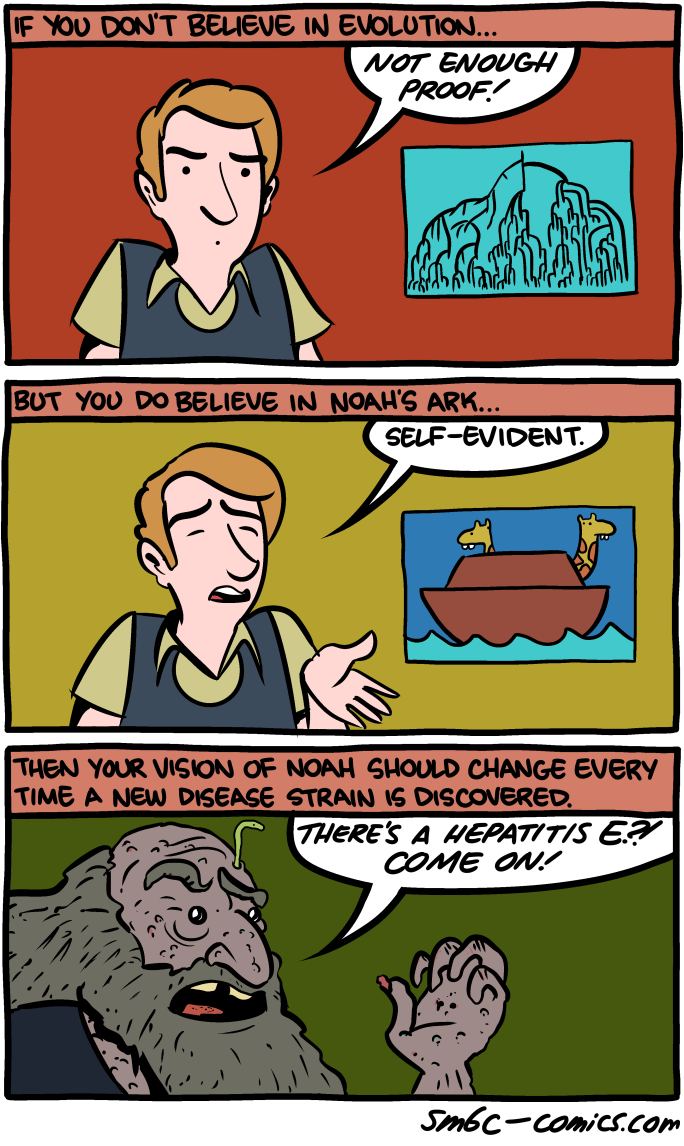
\includegraphics{./images/smbc-ID-evolution.png}
\caption{Even if one believes that pathogens evolve (at a high rate),
most human-only pathogens could have only survived a recent worldwide
flood such as the one described in Genesis by living on/in the surviving
humans. Source: smbc-comics.com (\url{http://www.smbc-comics.com/})}
\end{figure}

\section{Exercises}\label{exercises-13}

\begin{itemize}
\tightlist
\item
  The \emph{Evolutionary dynamics} app in the DSAIDE package provides
  hands-on computer exercises for this chapter.
\item
  Read the article `Evolutionary epidemiology 20 years on: Challenges
  and prospects' by Restif. The paper talks about 3 evolutionary
  patterns that are important to ID control. Find one or several papers
  that have been published in the last 5 years which address ID control
  from an evolutionary perspective of one or more of those topics
  mentioned in the Restif paper. Summarize and discuss the paper(s) you
  found. Critically assess the feasibility of the ideas put forward.
\end{itemize}

\section{Further Resources}\label{further-resources-13}

\begin{itemize}
\tightlist
\item
  The references mentioned in this chapter provide further information
  on specific topics.
\item
  Some clever ideas to fight and prevent drug resistance have recently
  been proposed, see (Baym, Stone, and Kishony
  \protect\hyperlink{ref-baym16}{2016}).
\item
  The interaction of co-infection (discussed in a previous chapter) and
  drug resistance is discussed in (Birger et al.
  \protect\hyperlink{ref-birger15}{2015}).
\item
  One of the primary goals in ID research is to be able to forecast the
  dynamics of ID, both on short and long timescales (similar to weather
  and climate forecasts). A review and discussion of that topic are in
  (Gandon et al. \protect\hyperlink{ref-gandon16}{2016}).
\end{itemize}

\section{References}\label{references-14}

\chapter{Emerging Infectious
Diseases}\label{emerging-infectious-diseases}

\section{Overview and Learning
Objectives}\label{overview-and-learning-objectives-14}

In this chapter, we will take a look at a specific evolutionary process
underlying the emergence of new Infectious Diseases

The learning objectives for this chapter are:

\begin{itemize}
\tightlist
\item
  Understand the central mechanisms and drivers of emergence
\end{itemize}

\section{Introduction}\label{introduction-13}

\section{Emergence and Evolution}\label{emergence-and-evolution}

For infectious diseases, you will often hear the term \emph{emergence}
as in \emph{Emerging Infectious Diseases}. This means the ID is in some
way new to a population, either never seen in a particular host before
(e.g., SARS emergence in 2003 in humans) or a disease that emerges in a
new location. The pathogen can either be an entirely new type (e.g.,
SARS, MERS) or a variant of an existing one (e.g., a new strain of
influenza or norovirus, or a drug-resistant form of a bacteria).
Emergence describes the observed phenomenon. Almost always in such
cases, some evolution occurs. For instance, a pathogen that is already
in the human population evolves drug resistance. Or a new pathogen is
introduced into the human population and then undergoes evolution to
adapt to the new host. While one could define emergence as the
phenomenon and evolution as the mechanism, in practice, you will often
find these terms used interchangeably, and the exact meaning will depend
on how the author defines it. In this chapter, we will discuss both the
mechanisms of evolution and how they can lead to the emergence of new
pathogens. The ability to understand and predict the emergence of new
IDs is, of course, of vital importance, recent references providing
additional information are (Brett, Drake, and Rohani
\protect\hyperlink{ref-brett17}{2017}; Dibble et al.
\protect\hyperlink{ref-dibble16}{2016}).

\section{Ecological drivers of evolution and
emergence}\label{ecological-drivers-of-evolution-and-emergence}

Many external, ecological factors affect ID dynamics. Weather, climate,
vegetation, the abundance and density of hosts and other species,
nutritional status, and general living conditions are all important
factors influencing human and animal ID. This is true both for
short-term dynamics (e.g., weather patterns can affect disease
incidence) as well as for the long-term evolutionary dynamics. The
emergence of many new viral pathogens among humans (e.g., HIV, SARS,
MERS) is likely caused by the closer contact humans have with the
animals who are the main hosts of those diseases. Transmission in these
situations of close human-animal contact is often called spillover.
Similarly, as discussed in the previous chapter, measles and other
diseases were only able to emerge and establish themselves among humans
once human populations became large enough. As global warming will
affect climate and as people become more affluent and urbanized, we can
expect further changes in ID dynamics and evolution over the next
decades - though predicting what changes exactly will occur, and which
diseases might increase and decrease in importance is very difficult
(Altizer et al. \protect\hyperlink{ref-altizer13}{2013}).

\section{Modeling ID Emergence
Dynamics}\label{modeling-id-emergence-dynamics}

To study evolutionary dynamics, we will need to implement models that
allow for changes in the system on top of the non-evolutionary dynamics
of the ID. Unless we plan to model many different potential new
variants, it is often easiest to pre-specify the number of variants we
want to track. In the simplest form where we only track pathogen
evolution, we might model the wild-type (normal, pre-existing) form of
the pathogen and a single mutant that is different in some important
characteristic, e.g., resistant to a drug or able to evade a vaccine. We
would build a model with these compartments. We often also pre-specify
the characteristics (i.e., the parameter values) for both the wild-type
and mutant. We implement the process of mutant generation in the model
and run the simulation. Under certain circumstances, we might see the
mutant be generated and take over the population.

If we want to model many different mutants, maybe allowing for random,
not pre-specified, differences in their fitness, and perhaps even
allowing for host evolution, the models get quite a bit more
complicated. They are not necessarily conceptually harder, but there is
more bookkeeping and coding involved making it technically trickier.

\section{Summary and Cartoon}\label{summary-and-cartoon-14}

This module provides a brief discussion of ID emergence.

\section{Exercises}\label{exercises-14}

\begin{itemize}
\item
\end{itemize}

\section{Further Resources}\label{further-resources-14}

\begin{itemize}
\item
\end{itemize}

\section{References}\label{references-15}

\chapter{Networks and ID}\label{networks-and-id}

\section{Overview and Learning
Objectives}\label{overview-and-learning-objectives-15}

In this module, we will briefly discuss the concept of transmission
networks and how that affects ID dynamics and control.

The learning objectives for this chapter are:

\begin{itemize}
\tightlist
\item
  Know the how to define and measure transmission networks
\item
  Understand how different types of network structures affect ID
  transmission and control
\item
  Understand how transmission networks affect disease spread
\item
  Evaluate the impact of network structure on ID transmission
\end{itemize}

\section{Introduction}\label{introduction-14}

ID spread along \emph{connections} between infected and uninfected
hosts. Those could be very close and defined connections, such as for
sexually transmitted infections, or much less well-defined connections,
such as a shared water or air source (e.g., cholera and influenza). If
we want to account for these connections explicitly, we need to consider
a conceptual framework that moves away from the compartmental approach.
In the compartmental approach, all hosts with given characteristics
(e.g., infected children) were lumped together, and no notion of
connectivity was included. In contrast, a network perspective explicitly
considers individuals and their connections.

\section{Network Terminology}\label{network-terminology}

The basic building blocks of networks are entities and their
connections. Those entities go by different, equivalent names, such as
actor, node, vertex, site. Similarly, the connections have different,
equivalent names, such as edge, link, bond, tie or connection. The
different names stem from the fact that the network framework was
developed independently in various scientific sub-fields.

\begin{figure}
\centering
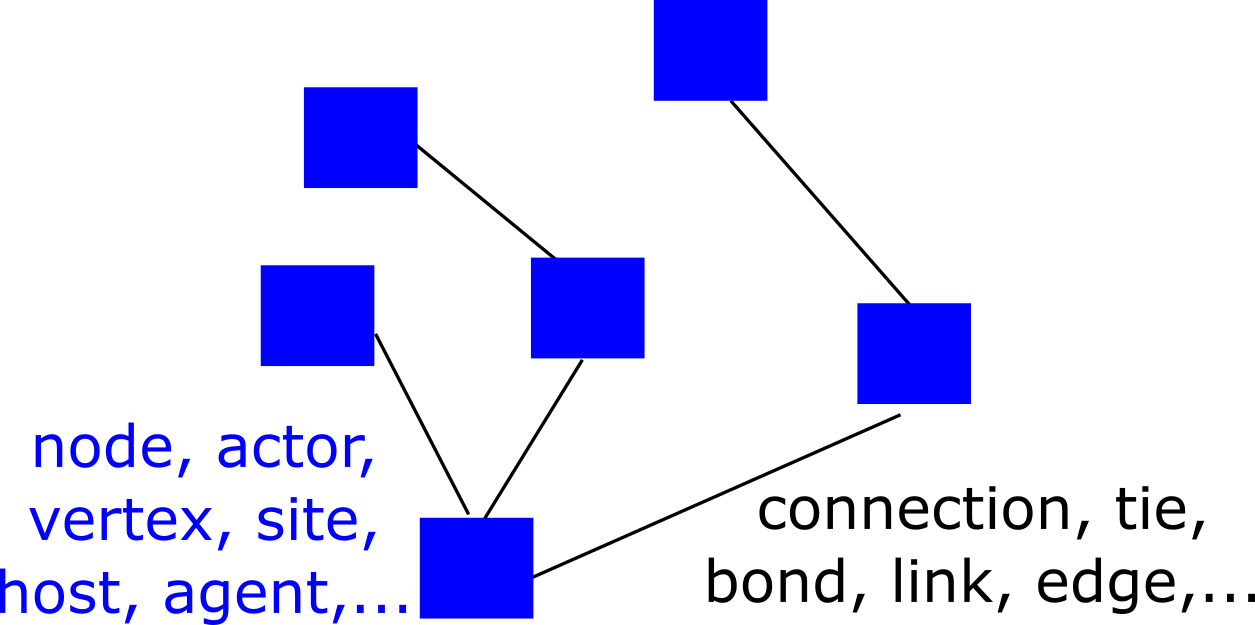
\includegraphics{./images/network-diagram.png}
\caption{Simple network diagram}
\end{figure}

\section{Network Nodes}\label{network-nodes}

Usually, the nodes are individual hosts (e.g., humans). But that does
not have to be the case. Nodes can also represent entities such as
schools, cities, hospitals, etc. Simple networks only have one type of
node, and more complicated networks can have different types of nodes.
For instance, humans can be connected to specific places where they
meet.

In their simplest form, nodes are only characterized by their
connections, and they don't have any other properties. In model
simulations, it is possible to give nodes features such as age, gender,
etc. and account for that when simulating ID spread.

\section{Network Connections}\label{network-connections}

What constitutes a connection in a network strongly depends on the
question asked and the ID under consideration. Sexual networks connect
people that have some form of sexual contact that was sufficient to
transmit the disease in question. Similarly, social contact networks
consider contacts between individuals in a social setting that allows
for the transmission of an ID, e.g., close contact for transmission of a
respiratory disease. Proximity networks can be built based on people
frequenting the same locations. Connections can either be simple or have
characteristics, which describe the relationship that exists between
nodes. For instance, connections can have weights, with stronger
connections between people that have closer or longer contacts.
Connections can also have directions. For instance, if we wanted to
model cholera transmission and had a network of villages, then a village
upstream would have a connection pointing to villages downstream, but
not the reverse. In other words, an `infected village' upstream can
infect a downstream village, but the opposite does not occur.

\begin{figure}
\centering
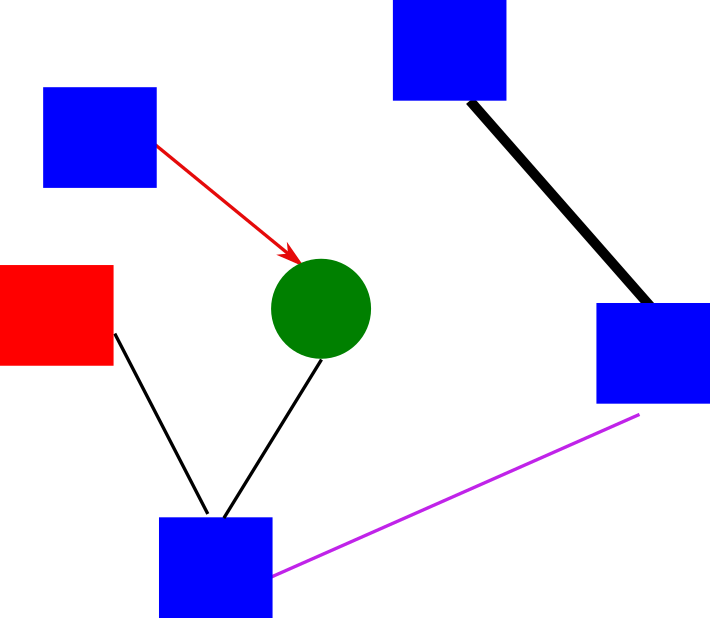
\includegraphics{./images/complex-network-diagram.png}
\caption{More complex network diagram showing different types of nodes
and connections.}
\end{figure}

\section{Network Characteristics}\label{network-characteristics}

The initial study of a network often starts with the properties of the
network itself, without considering any ID spread (yet). One of the most
important characteristics of a network is the degree distribution of the
nodes. This is simply a histogram of the number of connections that each
node has. If connections have directions or there is more than one type
of connection possible, then each one would have a histogram.

Another network characteristic is the `shortest path length', which
measures the shortest distance of going from a particular node to some
other node. Every node has a shortest path length to every other node
(if 2 nodes are not connected because they belong to unconnected
subparts of a network, the path length is considered infinite).

Many other network characteristics exist, the field of network analysis
has proliferated in the last several years. If you want to learn more,
(Newman \protect\hyperlink{ref-newman13}{2013}) is a useful resource.
Many review articles on that topic also exist (Keeling and Eames
\protect\hyperlink{ref-keeling05}{2005}).

It is important to understand that some characteristics are attached to
individual nodes and some to the full network. For instance, every node
has a number of degrees (connections), and the network has an overall
degree distribution. Similarly, one can compute the mean shortest path
length for each node and, if one takes another mean, a mean path length
for the whole network.

\section{Important types of networks}\label{important-types-of-networks}

There are several types or classes of networks with specific
characteristics that have been studied in great detail, either because
they are analytically tractable or because of their real-world
importance.

One of the best-studied networks is the random network. In this network,
any 2 nodes have a fixed probability of being connected. For a network
of \emph{N} nodes and connection probability \emph{p}, the average
number of connections each node has (it's degree) is \emph{(N-1)p}. The
degree distribution of the network is binomial, which for large networks
becomes a normal distribution. That means most nodes have approximately
the average number of connections. There are only a few nodes with
substantially fewer or more connections.

Many real-world networks do not have the degree distribution found for
random networks. It is often common that most nodes have very few
connections, while a few nodes have many connections. This idea, for
instance, underlies the superspreader concept. Such a distribution of
connections can be well described by a scale-free network. In which case
the degree distribution follows a power law, with most nodes having very
few connections but a small number of nodes having very many
connections.

\begin{figure}
\centering
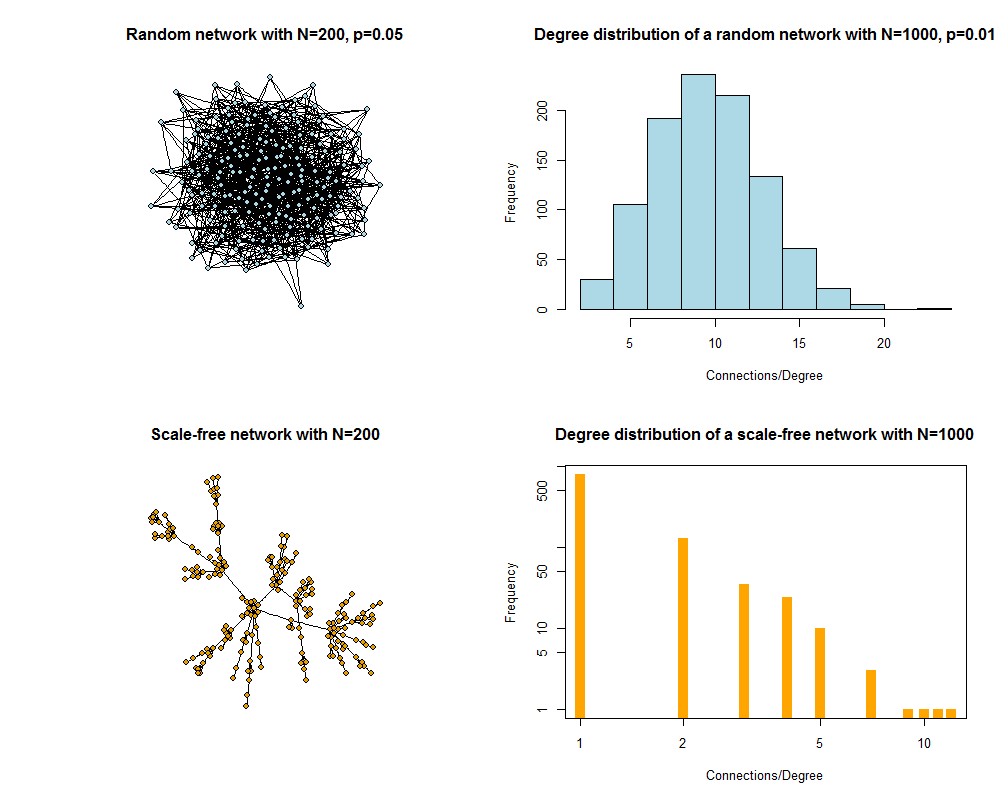
\includegraphics{./images/network-examples.png}
\caption{\label{fig:network-examples}Random and scale-free networks and
degree distribution.}
\end{figure}

\section{ID Transmission on Networks}\label{id-transmission-on-networks}

The premise for ID transmission is that it can only occur along the
connections of a network. As such, the structure of the network can
strongly influence the dynamics of the ID. How exactly different
characteristics of networks, such as the one discussed above and others,
interact with the features of the ID to affect overall ID dynamics is an
area that is currently heavily investigated. For some recent work on
that, see (Bansal, Grenfell, and Meyers
\protect\hyperlink{ref-bansal07}{2007}).

\section{Networks and ID Control}\label{networks-and-id-control}

Knowing about the connection structure is necessary for ID control. Most
obviously, if we are aware who the individuals are with many
connections, we could target them preferentially and have a potentially
larger impact compared to targeting random people. Other individuals
that connect separate clusters of a network might also be prime targets.
The challenge in real-world systems is to identify the individuals that
should be targeted and being able to reach them, and in an outbreak
situation, that would need to be done under time pressure. As such,
while network theory has much to offer for control, it is still
challenging to implement network-based intervention approaches in
practice.

\section{Modeling ID Transmission on
Networks}\label{modeling-id-transmission-on-networks}

Building and analyzing network models of ID transmission is generally
more challenging than the compartmental modeling approach. For networks,
we usually track individuals and as such the model becomes an
agent-based model caring all the added complexity associated with
agent-based modeling. It is also somewhat harder to analyze the results.
Still, networks are a much closer approximation of real systems and have
therefore seen increased use in the ID modeling community in recent
years. With an increase in available data of the `network type'
(geocoded cellphone data) further increases in computational power and
more sophisticated and efficient analysis approaches, it is quite likely
that network-based methods will continue to grow in importance.

\section{ID Transmission on Dynamic
Networks}\label{id-transmission-on-dynamic-networks}

Most of the time, networks are considered static and do not change
during the ID transmission process. However, this does not have to be
the case and is often not realistic. The most detailed models allow for
variations in the network through the making and breaking of connections
and addition and loss (birth and death) of nodes. Implementing and
analyzing models that have a dynamically changing network with the ID
dynamics (and potential control measures) occurring `on top' is
technically challenging. Not too many of such models currently exist,
but it is an area of active investigation by many, see (Bansal et al.
\protect\hyperlink{ref-bansal10}{2010}).

\section{Summary and Cartoon}\label{summary-and-cartoon-15}

This module provides a brief discussion of transmission networks and how
they impact dynamics and control of ID.

\begin{figure}
\centering
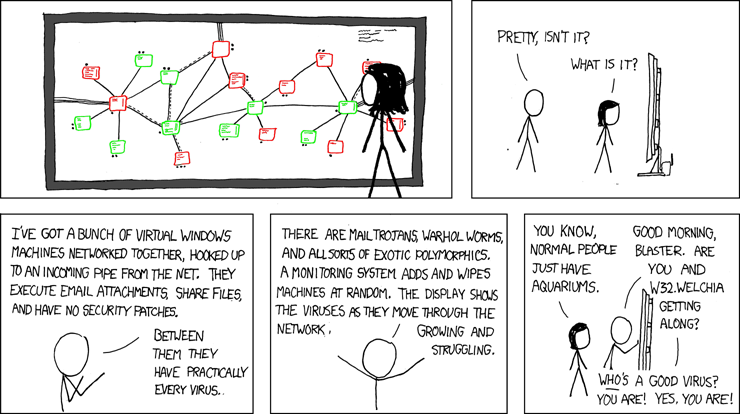
\includegraphics{./images/xkcd-network.png}
\caption{\label{fig:xkcdnetwork}Computer viruses and human viruses are in
many ways similar. \href{https://xkcd.com/350/}{Source: xkcd.com}.}
\end{figure}

\section{Exercises}\label{exercises-15}

\begin{itemize}
\tightlist
\item
  The online game \href{http://vax.herokuapp.com/}{VAX} provides a nice
  interactive setting where you can explore vaccination on networks and
  how it can help reduce disease spread. Try to pass all levels.
\item
  Find a study that looked at the dynamics of an ID on a network.
  Summarize and discuss the study. Explain what findings in the study
  are due to the network approach. Discuss/speculate how results would
  be different if one were to ignore the network structure and instead
  used a compartmental model approach.
\item
  Read the article ``Networks and epidemic models'' by Keeling and Eames
  (Keeling and Eames \protect\hyperlink{ref-keeling05}{2005}). Find a
  recent paper that investigates a network for some ID and explain which
  data collection approach of the ones mentioned in section 3 (or a
  different one) was used. Also, discuss the structure of the network
  that was observed in relation to the ones described in section 5.
\end{itemize}

\section{Further Resources}\label{further-resources-15}

\begin{itemize}
\tightlist
\item
  Nice general introductions to networks are given in {[}Strogatz
  (\protect\hyperlink{ref-strogatz01}{2001}); newman03{]}
\item
  Further discussion of networks and ID spread are provided in (Pellis
  et al. \protect\hyperlink{ref-pellis15}{2015}; Pastor-Satorras et al.
  \protect\hyperlink{ref-pastor-satorras15}{2015}; Ferrari et al.
  \protect\hyperlink{ref-ferrari11}{2011}; Bansal, Grenfell, and Meyers
  \protect\hyperlink{ref-bansal07}{2007})
\item
  Networks and ID control are for discussed in for instance (Salathé and
  Jones \protect\hyperlink{ref-salathe10}{2010}).
\end{itemize}

\section{References}\label{references-16}

\chapter{Summary}\label{summary}

This book provided an introduction to Infectious Disease Epidemiology
from a modern, dynamical systems perspective.

While the ability to be able to develop and analyze dynamical models
requires additional training and skills in mathematics and coding, I
hope that this book helped you to understand such a systems modeling
perspective and different ID concepts best discussed from such a
perspective.

\section{All References}\label{all-references}

\hypertarget{refs}{}
\hypertarget{ref-abu-raddad06}{}
Abu-Raddad, Laith J, Padmaja Patnaik, and James G Kublin. 2006. ``Dual
Infection with Hiv and Malaria Fuels the Spread of Both Diseases in
Sub-Saharan Africa.'' \emph{Science (New York, N.Y.)} 314 (5805):
1603--6.
doi:\href{https://doi.org/10.1126/science.1132338}{10.1126/science.1132338}.

\hypertarget{ref-altizer06}{}
Altizer, Sonia, Andrew Dobson, Parviez Hosseini, Peter Hudson, Mercedes
Pascual, and Pejman Rohani. 2006. ``Seasonality and the Dynamics of
Infectious Diseases.'' \emph{Ecology Letters} 9 (4): 467--84.
doi:\href{https://doi.org/10.1111/j.1461-0248.2005.00879.x}{10.1111/j.1461-0248.2005.00879.x}.

\hypertarget{ref-altizer13}{}
Altizer, Sonia, Richard S Ostfeld, Pieter T J Johnson, Susan Kutz, and C
Drew Harvell. 2013. ``Climate Change and Infectious Diseases: From
Evidence to a Predictive Framework.'' \emph{Science (New York, N.Y.)}
341 (6145): 514--19.
doi:\href{https://doi.org/10.1126/science.1239401}{10.1126/science.1239401}.

\hypertarget{ref-anderson91}{}
Anderson, Roy M, and RM May. 1991. ``Infectious Disease of Humans.''
\emph{Dynamics and Control}.

\hypertarget{ref-antia03}{}
Antia, Rustom, Roland R Regoes, Jacob C Koella, and Carl T Bergstrom.
2003. ``The Role of Evolution in the Emergence of Infectious Diseases.''
\emph{Nature} 426 (6967): 658--61.
doi:\href{https://doi.org/10.1038/nature02104}{10.1038/nature02104}.

\hypertarget{ref-bansal07}{}
Bansal, Shweta, Bryan T. Grenfell, and Lauren Ancel Meyers. 2007. ``When
Individual Behaviour Matters: Homogeneous and Network Models in
Epidemiology.'' \emph{J R Soc Interface} 4 (16). Computational; Applied
Mathematics, Institute for Computational Engineering; Sciences,
University of Texas at Austin, 1 University Station, C0200, Austin, TX
78712, USA.: 879--91.
doi:\href{https://doi.org/10.1098/rsif.2007.1100}{10.1098/rsif.2007.1100}.

\hypertarget{ref-bansal10}{}
Bansal, Shweta, Jonathan Read, Babak Pourbohloul, and Lauren Ancel
Meyers. 2010. ``The Dynamic Nature of Contact Networks in Infectious
Disease Epidemiology.'' \emph{J Biol Dyn} 4 (5). Center for Infectious
Disease Dynamics, The Pennsylvania State University, University Park,
PA, USA. shweta@sbansal.com: 478--89.
doi:\href{https://doi.org/10.1080/17513758.2010.503376}{10.1080/17513758.2010.503376}.

\hypertarget{ref-bartlett60}{}
Bartlett, M. S. 1960. ``The Critical Community Size for Measles in the
United States.'' \emph{Journal of the Royal Statistical Society. Series
A (General)} 123 (1): 37.
doi:\href{https://doi.org/10.2307/2343186}{10.2307/2343186}.

\hypertarget{ref-bartlett57}{}
Bartlett, Maurice S. 1957. ``Measles Periodicity and Community Size.''
\emph{Journal of the Royal Statistical Society. Series A (General)} 120
(1). JSTOR: 48--70.

\hypertarget{ref-basu13}{}
Basu, Sanjay, and Jason Andrews. 2013. ``Complexity in Mathematical
Models of Public Health Policies: A Guide for Consumers of Models.''
\emph{PLoS Medicine} 10 (10): e1001540.
doi:\href{https://doi.org/10.1371/journal.pmed.1001540}{10.1371/journal.pmed.1001540}.

\hypertarget{ref-baumgartner12}{}
Baumgartner, Eduardo, Christine N. Dao, Sharifa Nasreen, Mejbah Uddin
Bhuiyan, Syeda Mah-E-Muneer, Abdullah Al Mamun, M. A. Yushuf Sharker, et
al. 2012. ``Seasonality, Timing, and Climate Drivers of Influenza
Activity Worldwide.'' \emph{The Journal of Infectious Diseases} 206 (6):
838--46.
doi:\href{https://doi.org/10.1093/infdis/jis467}{10.1093/infdis/jis467}.

\hypertarget{ref-baym16}{}
Baym, M., L. K. Stone, and R. Kishony. 2016. ``Multidrug Evolutionary
Strategies to Reverse Antibiotic Resistance.'' \emph{Science} 351
(6268): aad3292--aad3292.
doi:\href{https://doi.org/10.1126/science.aad3292}{10.1126/science.aad3292}.

\hypertarget{ref-begon02}{}
Begon, M., M. Bennett, R. G. Bowers, N. P. French, S. M. Hazel, and J.
Turner. 2002. ``A Clarification of Transmission Terms in
Host-Microparasite Models: Numbers, Densities and Areas.''
\emph{Epidemiol Infect} 129 (1). ences, The University of Liverpool,
UK.: 147--53.

\hypertarget{ref-beldomenico09}{}
Beldomenico, Pablo M, Sandra Telfer, Stephanie Gebert, Lukasz Lukomski,
Malcolm Bennett, and Michael Begon. 2009. ``The Vicious Circle and
Infection Intensity: The Case of Trypanosoma Microti in Field Vole
Populations.'' \emph{Epidemics} 1 (3): 162--67.
doi:\href{https://doi.org/10.1016/j.epidem.2009.05.002}{10.1016/j.epidem.2009.05.002}.

\hypertarget{ref-birger15}{}
Birger, Ruthie B, Roger D Kouyos, Ted Cohen, Emily C Griffiths, Silvie
Huijben, Michael J Mina, Victoriya Volkova, Bryan Grenfell, and C
Jessica E Metcalf. 2015. ``The Potential Impact of Coinfection on
Antimicrobial Chemotherapy and Drug Resistance.'' \emph{Trends in
Microbiology} 23 (9): 537--44.
doi:\href{https://doi.org/10.1016/j.tim.2015.05.002}{10.1016/j.tim.2015.05.002}.

\hypertarget{ref-black12}{}
Black, Andrew J., and Alan J. McKane. 2012. ``Stochastic Formulation of
Ecological Models and Their Applications.'' \emph{Trends in Ecology \&
Evolution} 27 (6): 337--45.
doi:\href{https://doi.org/10.1016/j.tree.2012.01.014}{10.1016/j.tree.2012.01.014}.

\hypertarget{ref-black66}{}
Black, F L. 1966. ``Measles Endemicity in Insular Populations: Critical
Community Size and Its Evolutionary Implication.'' \emph{Journal of
Theoretical Biology} 11 (2): 207--11.

\hypertarget{ref-blower04}{}
Blower, Sally, and Daniel Bernoulli. 2004. ``An Attempt at a New
Analysis of the Mortality Caused by Smallpox and of the Advantages of
Inoculation to Prevent It. 1766.'' \emph{Reviews in Medical Virology} 14
(5): 275--88.

\hypertarget{ref-brankston07}{}
Brankston, Gabrielle, Leah Gitterman, Zahir Hirji, Camille Lemieux, and
Michael Gardam. 2007. ``Transmission of Influenza A in Human Beings.''
\emph{The Lancet Infectious Diseases} 7 (4): 257--65.
\url{http://www.sciencedirect.com/science/article/pii/S1473309907700294}.

\hypertarget{ref-brett17}{}
Brett, Tobias S, John M Drake, and Pejman Rohani. 2017. ``Anticipating
the Emergence of Infectious Diseases.'' \emph{Journal of the Royal
Society Interface} 14 (132). The Royal Society: 20170115.

\hypertarget{ref-britton10a}{}
Britton, Tom. 2010. ``Stochastic Epidemic Models: A Survey.''
\emph{Mathematical Biosciences} 225 (1): 24--35.
doi:\href{https://doi.org/10.1016/j.mbs.2010.01.006}{10.1016/j.mbs.2010.01.006}.

\hypertarget{ref-chen14}{}
Chen, Jennifer Y, Eoin R Feeney, and Raymond T Chung. 2014. ``HCV and
Hiv Co-Infection: Mechanisms and Management.'' \emph{Nature Reviews
Gastroenterology \& Hepatology} 11 (6). Nature Research: 362--71.

\hypertarget{ref-chubb10}{}
Chubb, Mikayla C., and Kathryn H. Jacobsen. 2010. ``Mathematical
Modeling and the Epidemiological Research Process.'' \emph{European
Journal of Epidemiology} 25 (1): 13--19.
doi:\href{https://doi.org/10.1007/s10654-009-9397-9}{10.1007/s10654-009-9397-9}.

\hypertarget{ref-contagionmovie}{}
``Contagion.'' 2011. Warner Bros.
\url{https://en.wikipedia.org/wiki/Contagion_(film)}.

\hypertarget{ref-cortez13}{}
Cortez, Michael H., and Joshua S. Weitz. 2013. ``Distinguishing Between
Indirect and Direct Modes of Transmission Using Epidemiological Time
Series.'' \emph{The American Naturalist} 181 (2): E43--E52.
doi:\href{https://doi.org/10.1086/668826}{10.1086/668826}.

\hypertarget{ref-davis12}{}
Davis, Brian M, Allison E Aiello, Suzanne Dawid, Pejman Rohani, Sourya
Shrestha, and Betsy Foxman. 2012. ``Influenza and Community-Acquired
Pneumonia Interactions: The Impact of Order and Time of Infection on
Population Patterns.'' \emph{American Journal of Epidemiology} 175 (5):
363--67.
doi:\href{https://doi.org/10.1093/aje/kwr402}{10.1093/aje/kwr402}.

\hypertarget{ref-dibble16}{}
Dibble, Christopher J, Eamon B O'Dea, Andrew W Park, and John M Drake.
2016. ``Waiting Time to Infectious Disease Emergence.'' \emph{Journal of
the Royal Society Interface} 13 (123). The Royal Society: 20160540.

\hypertarget{ref-diekmann10}{}
Diekmann, O., J A P. Heesterbeek, and M. G. Roberts. 2010. ``The
Construction of Next-Generation Matrices for Compartmental Epidemic
Models.'' \emph{J R Soc Interface} 7 (47). Department of Mathematics,
Utrecht University, Budapestlaan 6, 3584 CD, Utrecht, The Netherlands.:
873--85.
doi:\href{https://doi.org/10.1098/rsif.2009.0386}{10.1098/rsif.2009.0386}.

\hypertarget{ref-diekmann00}{}
Diekmann, Odo, and Johan Andre Peter Heesterbeek. 2000.
\emph{Mathematical Epidemiology of Infectious Diseases: Model Building,
Analysis and Interpretation}. Vol. 5. John Wiley \& Sons.

\hypertarget{ref-dowell01}{}
Dowell, S F. 2001. ``Seasonal Variation in Host Susceptibility and
Cycles of Certain Infectious Diseases.'' \emph{Emerging Infectious
Diseases} 7 (3): 369--74.
doi:\href{https://doi.org/10.3201/eid0703.010301}{10.3201/eid0703.010301}.

\hypertarget{ref-dushoff04}{}
Dushoff, Jonathan, Joshua B. Plotkin, Simon A. Levin, and David JD Earn.
2004. ``Dynamical Resonance Can Account for Seasonality of Influenza
Epidemics.'' \emph{Proceedings of the National Academy of Sciences of
the United States of America} 101 (48): 16915--6.
\url{http://www.pnas.org/content/101/48/16915.short}.

\hypertarget{ref-edmunds06}{}
Edmunds, W J, G Kafatos, J Wallinga, and J R Mossong. 2006. ``Mixing
Patterns and the Spread of Close-Contact Infectious Diseases.''
\emph{Emerging Themes in Epidemiology} 3 (August): 10.
doi:\href{https://doi.org/10.1186/1742-7622-3-10}{10.1186/1742-7622-3-10}.

\hypertarget{ref-emch08}{}
Emch, Michael, Caryl Feldacker, M Sirajul Islam, and Mohammad Ali. 2008.
``Seasonality of Cholera from 1974 to 2005: A Review of Global
Patterns.'' \emph{International Journal of Health Geographics} 7 (1):
31.
doi:\href{https://doi.org/10.1186/1476-072X-7-31}{10.1186/1476-072X-7-31}.

\hypertarget{ref-epstein08}{}
Epstein, Joshua M. 2008. ``Why Model?'' \emph{Journal of Artificial
Societies and Social Simulation} 11 (4): 12.
\url{http://jasss.soc.surrey.ac.uk/11/4/12.html}.

\hypertarget{ref-ewald87}{}
Ewald, P W. 1987. ``Transmission Modes and Evolution of the
Parasitism-Mutualism Continuum.'' \emph{Annals of the New York Academy
of Sciences} 503: 295--306.

\hypertarget{ref-ewald91}{}
---------. 1991. ``Waterborne Transmission and the Evolution of
Virulence Among Gastrointestinal Bacteria.'' \emph{Epidemiology and
Infection} 106 (1): 83--119.

\hypertarget{ref-ewald95}{}
---------. 1995. ``The Evolution of Virulence: A Unifying Link Between
Parasitology and Ecology.'' \emph{The Journal of Parasitology} 81 (5):
659--69.

\hypertarget{ref-ferguson16}{}
Ferguson, Neil M., Isabel Rodríguez-Barraquer, Ilaria Dorigatti, Luis
Mier-y-Teran-Romero, Daniel J. Laydon, and Derek AT Cummings. 2016.
``Benefits and Risks of the Sanofi-Pasteur Dengue Vaccine: Modeling
Optimal Deployment.'' \emph{Science} 353 (6303): 1033--6.
\url{http://science.sciencemag.org/content/353/6303/1033.short}.

\hypertarget{ref-ferrari11}{}
Ferrari, Matthew J., Sarah E. Perkins, Laura W. Pomeroy, and Ottar N.
Bjørnstad. 2011. ``Pathogens, Social Networks, and the Paradox of
Transmission Scaling.'' \emph{Interdisciplinary Perspectives on
Infectious Diseases} 2011: 1--10.
doi:\href{https://doi.org/10.1155/2011/267049}{10.1155/2011/267049}.

\hypertarget{ref-fine03}{}
Fine, P. E. M. 2003. ``The Interval Between Successive Cases of an
Infectious Disease.'' \emph{American Journal of Epidemiology} 158 (11):
1039--47.
doi:\href{https://doi.org/10.1093/aje/kwg251}{10.1093/aje/kwg251}.

\hypertarget{ref-fine93}{}
Fine, Paul EM. 1993. ``Herd Immunity: History, Theory, Practice.''
\emph{Epidemiologic Reviews} 15 (2): 265--302.
\url{http://op12no2.me/stuff/herdhis.pdf}.

\hypertarget{ref-fine11}{}
Fine, Paul, Ken Eames, and David L Heymann. 2011. ```Herd Immunity': A
Rough Guide.'' \emph{Clinical Infectious Diseases : An Official
Publication of the Infectious Diseases Society of America} 52 (7):
911--16.
doi:\href{https://doi.org/10.1093/cid/cir007}{10.1093/cid/cir007}.

\hypertarget{ref-frank07}{}
Frank, Steven A, and Robin M Bush. 2007. ``Barriers to Antigenic Escape
by Pathogens: Trade-Off Between Reproductive Rate and Antigenic
Mutability.'' \emph{BMC Evolutionary Biology} 7 (November): 229.
doi:\href{https://doi.org/10.1186/1471-2148-7-229}{10.1186/1471-2148-7-229}.

\hypertarget{ref-galvani05}{}
Galvani, Alison P., and Robert M. May. 2005. ``Epidemiology: Dimensions
of Superspreading.'' \emph{Nature} 438 (7066): 293--95.
doi:\href{https://doi.org/10.1038/438293a}{10.1038/438293a}.

\hypertarget{ref-gandon16}{}
Gandon, Sylvain, Troy Day, C. Jessica E. Metcalf, and Bryan T. Grenfell.
2016. ``Forecasting Epidemiological and Evolutionary Dynamics of
Infectious Diseases.'' \emph{Trends in Ecology \& Evolution} 31 (10):
776--88.
doi:\href{https://doi.org/10.1016/j.tree.2016.07.010}{10.1016/j.tree.2016.07.010}.

\hypertarget{ref-garnett11}{}
Garnett, Geoffrey P., Simon Cousens, Timothy B. Hallett, Richard
Steketee, and Neff Walker. 2011. ``Mathematical Models in the Evaluation
of Health Programmes.'' \emph{The Lancet} 378 (9790): 515--25.
\url{http://www.sciencedirect.com/science/article/pii/S014067361061505X}.

\hypertarget{ref-giesecke17}{}
Giesecke, Johan. 2017. \emph{Modern Infectious Disease Epidemiology}.
CRC Press.

\hypertarget{ref-grassly06}{}
Grassly, Nicholas C, and Christophe Fraser. 2006. ``Seasonal Infectious
Disease Epidemiology.'' \emph{Proceedings of the Royal Society of London
B: Biological Sciences} 273 (1600). The Royal Society: 2541--50.

\hypertarget{ref-griffiths11}{}
Griffiths, Emily C, Amy B Pedersen, Andy Fenton, and Owen L Petchey.
2011. ``The Nature and Consequences of Coinfection in Humans.''
\emph{Journal of Infection} 63 (3). Elsevier: 200--206.

\hypertarget{ref-gunawardena14}{}
Gunawardena, Jeremy. 2014. ``Models in Biology:`accurate Descriptions of
Our Pathetic Thinking'.'' \emph{BMC Biology} 12 (1): 29.
\url{https://bmcbiol.biomedcentral.com/articles/10.1186/1741-7007-12-29}.

\hypertarget{ref-halloran14}{}
Halloran, M. E., and I. M. Longini. 2014. ``Emerging, Evolving, and
Established Infectious Diseases and Interventions.'' \emph{Science} 345
(6202): 1292--4.
doi:\href{https://doi.org/10.1126/science.1254166}{10.1126/science.1254166}.

\hypertarget{ref-heesterbeek15}{}
Heesterbeek, H., R. M. Anderson, V. Andreasen, S. Bansal, D. De Angelis,
C. Dye, K. T. D. Eames, et al. 2015. ``Modeling Infectious Disease
Dynamics in the Complex Landscape of Global Health.'' \emph{Science} 347
(6227): aaa4339--aaa4339.
doi:\href{https://doi.org/10.1126/science.aaa4339}{10.1126/science.aaa4339}.

\hypertarget{ref-heffernan05}{}
Heffernan, J M, R J Smith, and L M Wahl. 2005. ``Perspectives on the
Basic Reproductive Ratio.'' \emph{Journal of the Royal Society,
Interface} 2 (4): 281--93.
doi:\href{https://doi.org/10.1098/rsif.2005.0042}{10.1098/rsif.2005.0042}.

\hypertarget{ref-homer06}{}
Homer, Jack B., and Gary B. Hirsch. 2006. ``System Dynamics Modeling for
Public Health: Background and Opportunities.'' \emph{American Journal of
Public Health} 96 (3): 452--58.
\url{http://ajph.aphapublications.org/doi/abs/10.2105/AJPH.2005.062059}.

\hypertarget{ref-kajita07}{}
Kajita, Emily, Justin T Okano, Erin N Bodine, Scott P Layne, and Sally
Blower. 2007. ``Modelling an Outbreak of an Emerging Pathogen.''
\emph{Nature Reviews. Microbiology} 5 (9): 700--709.
doi:\href{https://doi.org/10.1038/nrmicro1660}{10.1038/nrmicro1660}.

\hypertarget{ref-karp07a}{}
Karp, Christopher L, and Paul G Auwaerter. 2007a. ``Coinfection with Hiv
and Tropical Infectious Diseases. I. Protozoal Pathogens.''
\emph{Clinical Infectious Diseases : An Official Publication of the
Infectious Diseases Society of America} 45 (9): 1208--13.
doi:\href{https://doi.org/10.1086/522181}{10.1086/522181}.

\hypertarget{ref-karp07}{}
---------. 2007b. ``Coinfection with Hiv and Tropical Infectious
Diseases. Ii. Helminthic, Fungal, Bacterial, and Viral Pathogens.''
\emph{Clinical Infectious Diseases : An Official Publication of the
Infectious Diseases Society of America} 45 (9): 1214--20.
doi:\href{https://doi.org/10.1086/522180}{10.1086/522180}.

\hypertarget{ref-keeling97}{}
Keeling, M J. 1997. ``Modelling the Persistence of Measles.''
\emph{Trends in Microbiology} 5 (12): 513--18.
doi:\href{https://doi.org/10.1016/S0966-842X(97)01147-5}{10.1016/S0966-842X(97)01147-5}.

\hypertarget{ref-keeling97a}{}
Keeling, M. J. 1997. ``Disease Extinction and Community Size: Modeling
the Persistence of Measles.'' \emph{Science} 275 (5296): 65--67.
doi:\href{https://doi.org/10.1126/science.275.5296.65}{10.1126/science.275.5296.65}.

\hypertarget{ref-keeling09}{}
Keeling, M. J., and L. Danon. 2009. ``Mathematical Modelling of
Infectious Diseases.'' \emph{British Medical Bulletin} 92 (1): 33--42.
doi:\href{https://doi.org/10.1093/bmb/ldp038}{10.1093/bmb/ldp038}.

\hypertarget{ref-keeling02}{}
Keeling, Matt J, and Bryan T Grenfell. 2002. ``Understanding the
Persistence of Measles: Reconciling Theory, Simulation and
Observation.'' \emph{Proceedings. Biological Sciences / the Royal
Society} 269 (1489): 335--43.

\hypertarget{ref-keeling08}{}
Keeling, Matt J, and Pejman Rohani. 2008. \emph{Modeling Infectious
Diseases in Humans and Animals}. Princeton University Press.

\hypertarget{ref-keeling05}{}
Keeling, Matt J., and Ken T D. Eames. 2005. ``Networks and Epidemic
Models.'' \emph{J R Soc Interface} 2 (4). Mathematics, University of
Warwick, Institute Gibbet Hill Road, Coventry CV4 7AL, UK.
m.j.keeling@warwick.ac.uk: 295--307.
doi:\href{https://doi.org/10.1098/rsif.2005.0051}{10.1098/rsif.2005.0051}.

\hypertarget{ref-kilpatrick12}{}
Kilpatrick, A Marm, and Sarah E Randolph. 2012. ``Drivers, Dynamics, and
Control of Emerging Vector-Borne Zoonotic Diseases.'' \emph{Lancet
(London, England)} 380 (9857): 1946--55.
doi:\href{https://doi.org/10.1016/S0140-6736(12)61151-9}{10.1016/S0140-6736(12)61151-9}.

\hypertarget{ref-kim09}{}
Kim, Arthur Y, and Raymond T Chung. 2009. ``Coinfection with Hiv-1 and
Hcv---a One-Two Punch.'' \emph{Gastroenterology} 137 (3). Elsevier:
795--814.

\hypertarget{ref-king08}{}
King, Aaron A., Edward L. Ionides, Mercedes Pascual, and Menno J. Bouma.
2008. ``Inapparent Infections and Cholera Dynamics.'' \emph{Nature} 454
(7206): 877--80.
doi:\href{https://doi.org/10.1038/nature07084}{10.1038/nature07084}.

\hypertarget{ref-klepac13}{}
Klepac, Petra, C Jessica E Metcalf, Angela R McLean, and Katie Hampson.
2013. ``Towards the Endgame and Beyond: Complexities and Challenges for
the Elimination of Infectious Diseases.'' \emph{Philosophical
Transactions of the Royal Society of London. Series B, Biological
Sciences} 368 (1623): 20120137.
doi:\href{https://doi.org/10.1098/rstb.2012.0137}{10.1098/rstb.2012.0137}.

\hypertarget{ref-lange09}{}
Lange, Alexander, and Neil M Ferguson. 2009. ``Antigenic Diversity,
Transmission Mechanisms, and the Evolution of Pathogens.'' \emph{PLoS
Computational Biology} 5 (10): e1000536.
doi:\href{https://doi.org/10.1371/journal.pcbi.1000536}{10.1371/journal.pcbi.1000536}.

\hypertarget{ref-lessler16}{}
Lessler, Justin, Andrew S. Azman, M. Kate Grabowski, Henrik Salje, and
Isabel Rodriguez-Barraquer. 2016. ``Trends in the Mechanistic and
Dynamic Modeling of Infectious Diseases.'' \emph{Current Epidemiology
Reports} 3 (3): 212--22.
doi:\href{https://doi.org/10.1007/s40471-016-0078-4}{10.1007/s40471-016-0078-4}.

\hypertarget{ref-levy04}{}
Levy, Stuart B, and Bonnie Marshall. 2004. ``Antibacterial Resistance
Worldwide: Causes, Challenges and Responses.'' \emph{Nature Medicine} 10
(12s): S122--S129.
doi:\href{https://doi.org/10.1038/nm1145}{10.1038/nm1145}.

\hypertarget{ref-li11}{}
Li, Jing, Daniel Blakeley, and Robert J. Smith. 2011. ``The Failure of R
0.'' \emph{Computational and Mathematical Methods in Medicine} 2011:
1--17.
doi:\href{https://doi.org/10.1155/2011/527610}{10.1155/2011/527610}.

\hypertarget{ref-li13}{}
Li, Xin-Xu, and Xiao-Nong Zhou. 2013. ``Co-Infection of Tuberculosis and
Parasitic Diseases in Humans: A Systematic Review.'' \emph{Parasites \&
Vectors} 6 (March): 79.
doi:\href{https://doi.org/10.1186/1756-3305-6-79}{10.1186/1756-3305-6-79}.

\hypertarget{ref-lipsitch09}{}
Lipsitch, Marc, and Cécile Viboud. 2009. ``Influenza Seasonality:
Lifting the Fog.'' \emph{Proc Natl Acad Sci U S A} 106 (10). Department
of Epidemiology, Harvard School of Public Health, Boston, MA 02130, USA.
mlipsitc@hsph.harvard.edu: 3645--6.
doi:\href{https://doi.org/10.1073/pnas.0900933106}{10.1073/pnas.0900933106}.

\hypertarget{ref-lloyd-smith05}{}
Lloyd-Smith, J. O., S. J. Schreiber, P. E. Kopp, and W. M. Getz. 2005.
``Superspreading and the Effect of Individual Variation on Disease
Emergence.'' \emph{Nature} 438 (7066). Department of Environmental
Science, Policy; Management, 140 Mulford Hall, University of California,
Berkeley, California 94720-3114, USA. jls@nature.berkeley.edu: 355--59.
doi:\href{https://doi.org/10.1038/nature04153}{10.1038/nature04153}.

\hypertarget{ref-lloyd-smith05b}{}
Lloyd-Smith, James O, Paul C Cross, Cheryl J Briggs, Matt Daugherty,
Wayne M Getz, John Latto, Maria S Sanchez, Adam B Smith, and Andrea
Swei. 2005. ``Should We Expect Population Thresholds for Wildlife
Disease?'' \emph{Trends in Ecology \& Evolution} 20 (9): 511--19.
doi:\href{https://doi.org/10.1016/j.tree.2005.07.004}{10.1016/j.tree.2005.07.004}.

\hypertarget{ref-lofgren07}{}
Lofgren, E., N. H. Fefferman, Y. N. Naumov, J. Gorski, and E. N.
Naumova. 2007. ``Influenza Seasonality: Underlying Causes and Modeling
Theories.'' \emph{Journal of Virology} 81 (11): 5429--36.
doi:\href{https://doi.org/10.1128/JVI.01680-06}{10.1128/JVI.01680-06}.

\hypertarget{ref-louz10}{}
Louz, Derrick, Hans E. Bergmans, Birgit P. Loos, and Rob C. Hoeben.
2010. ``Emergence of Viral Diseases: Mathematical Modeling as a Tool for
Infection Control, Policy and Decision Making.'' \emph{Critical Reviews
in Microbiology} 36 (3): 195--211.
doi:\href{https://doi.org/10.3109/10408411003604619}{10.3109/10408411003604619}.

\hypertarget{ref-luke12}{}
Luke, Douglas A, and Katherine A Stamatakis. 2012. ``Systems Science
Methods in Public Health: Dynamics, Networks, and Agents.'' \emph{Annual
Review of Public Health} 33. Annual Reviews: 357--76.

\hypertarget{ref-luz10}{}
Luz, Paula M, Claudio J Struchiner, and Alison P Galvani. 2010.
``Modeling Transmission Dynamics and Control of Vector-Borne Neglected
Tropical Diseases.'' \emph{PLoS Neglected Tropical Diseases} 4 (10):
e761.
doi:\href{https://doi.org/10.1371/journal.pntd.0000761}{10.1371/journal.pntd.0000761}.

\hypertarget{ref-ma06}{}
Ma, Junling, and David JD Earn. 2006. ``Generality of the Final Size
Formula for an Epidemic of a Newly Invading Infectious Disease.''
\emph{Bulletin of Mathematical Biology} 68 (3). Springer: 679--702.

\hypertarget{ref-matthews05}{}
Matthews, Louise, and Mark Woolhouse. 2005. ``New Approaches to
Quantifying the Spread of Infection.'' \emph{Nature Reviews.
Microbiology} 3 (7): 529--36.
doi:\href{https://doi.org/10.1038/nrmicro1178}{10.1038/nrmicro1178}.

\hypertarget{ref-may04}{}
May, R. M. 2004. ``Uses and Abuses of Mathematics in Biology.''
\emph{Science} 303 (5659): 790--93.
doi:\href{https://doi.org/10.1126/science.1094442}{10.1126/science.1094442}.

\hypertarget{ref-may01}{}
May, Robert M, Sunetra Gupta, and Angela R McLean. 2001. ``Infectious
Disease Dynamics: What Characterizes a Successful Invader?''
\emph{Philosophical Transactions of the Royal Society of London B:
Biological Sciences} 356 (1410). The Royal Society: 901--10.

\hypertarget{ref-mccallum01}{}
McCallum, H., N. Barlow, and J. Hone. 2001. ``How Should Pathogen
Transmission Be Modelled?'' \emph{Trends Ecol Evol} 16 (6): 295--300.

\hypertarget{ref-mccallum17}{}
McCallum, Hamish, Andy Fenton, Peter J Hudson, Brian Lee, Beth Levick,
Rachel Norman, Sarah E Perkins, Mark Viney, Anthony J Wilson, and Joanne
Lello. 2017. ``Breaking Beta: Deconstructing the Parasite Transmission
Function.'' \emph{Philosophical Transactions of the Royal Society of
London. Series B, Biological Sciences} 372 (1719).
doi:\href{https://doi.org/10.1098/rstb.2016.0084}{10.1098/rstb.2016.0084}.

\hypertarget{ref-mccullers06}{}
McCullers, Jonathan A. 2006. ``Insights into the Interaction Between
Influenza Virus and Pneumococcus.'' \emph{Clinical Microbiology Reviews}
19 (3): 571--82.
doi:\href{https://doi.org/10.1128/CMR.00058-05}{10.1128/CMR.00058-05}.

\hypertarget{ref-metcalf15}{}
Metcalf, C J E, W J Edmunds, and J Lessler. 2015. ``Six Challenges in
Modelling for Public Health Policy.'' \emph{Epidemics} 10 (March):
93--96.
doi:\href{https://doi.org/10.1016/j.epidem.2014.08.008}{10.1016/j.epidem.2014.08.008}.

\hypertarget{ref-metcalf17}{}
Metcalf, C Jessica E, and Justin Lessler. 2017. ``Opportunities and
Challenges in Modeling Emerging Infectious Diseases.'' \emph{Science
(New York, N.Y.)} 357 (6347): 149--52.
doi:\href{https://doi.org/10.1126/science.aam8335}{10.1126/science.aam8335}.

\hypertarget{ref-milwid16}{}
Milwid, Rachael, Andreea Steriu, Julien Arino, Jane Heffernan, Ayaz
Hyder, Dena Schanzer, Emma Gardner, et al. 2016. ``Toward Standardizing
a Lexicon of Infectious Disease Modeling Terms.'' \emph{Frontiers in
Public Health} 4: 213.
doi:\href{https://doi.org/10.3389/fpubh.2016.00213}{10.3389/fpubh.2016.00213}.

\hypertarget{ref-mina15}{}
Mina, Michael J, C Jessica E Metcalf, Rik L de Swart, A D M E Osterhaus,
and Bryan T Grenfell. 2015. ``Long-Term Measles-Induced Immunomodulation
Increases Overall Childhood Infectious Disease Mortality.''
\emph{Science (New York, N.Y.)} 348 (6235): 694--99.
doi:\href{https://doi.org/10.1126/science.aaa3662}{10.1126/science.aaa3662}.

\hypertarget{ref-mossong08}{}
Mossong, Joël, Niel Hens, Mark Jit, Philippe Beutels, Kari Auranen,
Rafael Mikolajczyk, Marco Massari, et al. 2008. ``Social Contacts and
Mixing Patterns Relevant to the Spread of Infectious Diseases.''
\emph{PLoS Medicine} 5 (3): e74.
\url{http://journals.plos.org/plosmedicine/article?id=10.1371/journal.pmed.0050074}.

\hypertarget{ref-nelson13}{}
Nelson, Kenrad E, and Carolyn Williams. 2013. \emph{Infectious Disease
Epidemiology}. Jones \& Bartlett Publishers.

\hypertarget{ref-ness07}{}
Ness, Roberta B., James S. Koopman, and Mark S. Roberts. 2007. ``Causal
System Modeling in Chronic Disease Epidemiology: A Proposal.''
\emph{Annals of Epidemiology} 17 (7): 564--68.
doi:\href{https://doi.org/10.1016/j.annepidem.2006.10.014}{10.1016/j.annepidem.2006.10.014}.

\hypertarget{ref-newman13}{}
Newman, M. E. J. 2013. \emph{Networks: An Introduction}. Reprint. with
corr. Oxford {[}u.a.{]}: Oxford Univ. Press.

\hypertarget{ref-pascual02}{}
Pascual, Mercedes, Menno J. Bouma, and Andrew P. Dobson. 2002. ``Cholera
and Climate: Revisiting the Quantitative Evidence.'' \emph{Microbes and
Infection} 4 (2): 237--45.
\url{http://www.sciencedirect.com/science/article/pii/S1286457901015337}.

\hypertarget{ref-pastor-satorras15}{}
Pastor-Satorras, Romualdo, Claudio Castellano, Piet Van Mieghem, and
Alessandro Vespignani. 2015. ``Epidemic Processes in Complex Networks.''
\emph{Reviews of Modern Physics} 87 (3): 925--79.
doi:\href{https://doi.org/10.1103/RevModPhys.87.925}{10.1103/RevModPhys.87.925}.

\hypertarget{ref-paull12}{}
Paull, Sara H, Sejin Song, Katherine M McClure, Loren C Sackett, A Marm
Kilpatrick, and Pieter TJ Johnson. 2012. ``From Superspreaders to
Disease Hotspots: Linking Transmission Across Hosts and Space.''
\emph{Frontiers in Ecology and the Environment} 10 (2). Wiley Online
Library: 75--82.

\hypertarget{ref-pawlowski12}{}
Pawlowski, Andrzej, Marianne Jansson, Markus Sköld, Martin E Rottenberg,
and Gunilla Källenius. 2012. ``Tuberculosis and Hiv Co-Infection.''
\emph{PLoS Pathogens} 8 (2): e1002464.
doi:\href{https://doi.org/10.1371/journal.ppat.1002464}{10.1371/journal.ppat.1002464}.

\hypertarget{ref-peel14}{}
Peel, A J, J R C Pulliam, A D Luis, R K Plowright, T J O'Shea, D T S
Hayman, J L N Wood, C T Webb, and O Restif. 2014. ``The Effect of
Seasonal Birth Pulses on Pathogen Persistence in Wild Mammal
Populations.'' \emph{Proceedings. Biological Sciences} 281 (1786).
doi:\href{https://doi.org/10.1098/rspb.2013.2962}{10.1098/rspb.2013.2962}.

\hypertarget{ref-pellis15}{}
Pellis, Lorenzo, Frank Ball, Shweta Bansal, Ken Eames, Thomas House,
Valerie Isham, and Pieter Trapman. 2015. ``Eight Challenges for Network
Epidemic Models.'' \emph{Epidemics} 10 (March): 58--62.
doi:\href{https://doi.org/10.1016/j.epidem.2014.07.003}{10.1016/j.epidem.2014.07.003}.

\hypertarget{ref-peters14}{}
Peters, David H. 2014. ``The Application of Systems Thinking in Health:
Why Use Systems Thinking?'' \emph{Health Research Policy and Systems} 12
(1): 51.
\url{https://health-policy-systems.biomedcentral.com/articles/10.1186/1478-4505-12-51}.

\hypertarget{ref-petney98}{}
Petney, Trevor N, and Ross H Andrews. 1998. ``Multiparasite Communities
in Animals and Humans: Frequency, Structure and Pathogenic
Significance.'' \emph{International Journal for Parasitology} 28 (3).
Elsevier: 377--93.

\hypertarget{ref-pittman16}{}
Pittman, Kelly J., Luke C. Glover, Liuyang Wang, and Dennis C. Ko. 2016.
``The Legacy of Past Pandemics: Common Human Mutations That Protect
Against Infectious Disease.'' Edited by William E. Goldman. \emph{PLOS
Pathogens} 12 (7): e1005680.
doi:\href{https://doi.org/10.1371/journal.ppat.1005680}{10.1371/journal.ppat.1005680}.

\hypertarget{ref-potterat99}{}
Potterat, John J., Helen Zimmerman-Rogers, Stephen Q. Muth, Richard B.
Rothenberg, David L. Green, Jerry E. Taylor, Mandy S. Bonney, and Helen
A. White. 1999. ``Chlamydia Transmission: Concurrency, Reproduction
Number, and the Epidemic Trajectory.'' \emph{American Journal of
Epidemiology} 150 (12): 1331--9.
\url{https://academic.oup.com/aje/article-abstract/150/12/1331/53233}.

\hypertarget{ref-roberts07}{}
Roberts, M G. 2007. ``The Pluses and Minuses of R0.'' \emph{Journal of
the Royal Society, Interface} 4 (16): 949--61.
doi:\href{https://doi.org/10.1098/rsif.2007.1031}{10.1098/rsif.2007.1031}.

\hypertarget{ref-rohani03}{}
Rohani, P, CJ Green, NB Mantilla-Beniers, and BT Grenfell. 2003.
``Ecological Interference Between Fatal Diseases.'' \emph{Nature} 422
(6934). Nature Publishing Group: 885.

\hypertarget{ref-salathe10}{}
Salathé, Marcel, and James H. Jones. 2010. ``Dynamics and Control of
Diseases in Networks with Community Structure.'' \emph{PLoS
Computational Biology} 6 (4): e1000736.
\url{http://journals.plos.org/ploscompbiol/article?id=10.1371/journal.pcbi.1000736}.

\hypertarget{ref-sanchez-romero16}{}
Sánchez-Romero, Luz Maria, Joanne Penko, Pamela G. Coxson, Alicia
Fernández, Antoinette Mason, Andrew E. Moran, Leticia Ávila-Burgos,
Michelle Odden, Simón Barquera, and Kirsten Bibbins-Domingo. 2016.
``Projected Impact of Mexico's Sugar-Sweetened Beverage Tax Policy on
Diabetes and Cardiovascular Disease: A Modeling Study.'' \emph{PLoS
Medicine} 13 (11): e1002158.
\url{http://journals.plos.org/plosmedicine/article?id=10.1371/journal.pmed.1002158}.

\hypertarget{ref-shaman10}{}
Shaman, Jeffrey, Virginia E. Pitzer, Cécile Viboud, Bryan T. Grenfell,
and Marc Lipsitch. 2010. ``Absolute Humidity and the Seasonal Onset of
Influenza in the Continental United States.'' \emph{PLoS Biol} 8 (2).
College of Oceanic; Atmospheric Sciences, Oregon State University,
Corvallis, Oregon, United States of America.: e1000316.
doi:\href{https://doi.org/10.1371/journal.pbio.1000316}{10.1371/journal.pbio.1000316}.

\hypertarget{ref-shrestha13}{}
Shrestha, Sourya, Betsy Foxman, Suzanne Dawid, Allison E Aiello, Brian M
Davis, Joshua Berus, and Pejman Rohani. 2013. ``Time and Dose-Dependent
Risk of Pneumococcal Pneumonia Following Influenza: A Model for
Within-Host Interaction Between Influenza and Streptococcus
Pneumoniae.'' \emph{Journal of the Royal Society, Interface} 10 (86):
20130233.
doi:\href{https://doi.org/10.1098/rsif.2013.0233}{10.1098/rsif.2013.0233}.

\hypertarget{ref-smith14a}{}
Smith, Amber M, and Jonathan A McCullers. 2014. ``Secondary Bacterial
Infections in Influenza Virus Infection Pathogenesis.'' \emph{Current
Topics in Microbiology and Immunology} 385: 327--56.
doi:\href{https://doi.org/10.1007/82_2014_394}{10.1007/82\_2014\_394}.

\hypertarget{ref-smith14}{}
Smith, David L, T Alex Perkins, Robert C Reiner, Christopher M Barker,
Tianchan Niu, Luis Fernando Chaves, Alicia M Ellis, et al. 2014.
``Recasting the Theory of Mosquito-Borne Pathogen Transmission Dynamics
and Control.'' \emph{Transactions of the Royal Society of Tropical
Medicine and Hygiene} 108 (4): 185--97.
doi:\href{https://doi.org/10.1093/trstmh/tru026}{10.1093/trstmh/tru026}.

\hypertarget{ref-epimooc}{}
State, Penn. 2014. ``Epidemics - the Dynamics of Infectious Diseases.''
\url{https://www.coursera.org/learn/epidemics}.

\hypertarget{ref-stein11}{}
Stein, Richard A. 2011. ``Super-Spreaders in Infectious Diseases.''
\emph{International Journal of Infectious Diseases : IJID : Official
Publication of the International Society for Infectious Diseases} 15
(8): e510--e513.
doi:\href{https://doi.org/10.1016/j.ijid.2010.06.020}{10.1016/j.ijid.2010.06.020}.

\hypertarget{ref-sterman06}{}
Sterman, John D. 2006. ``Learning from Evidence in a Complex World.''
\emph{American Journal of Public Health} 96 (3): 505--14.
\url{http://ajph.aphapublications.org/doi/abs/10.2105/AJPH.2005.066043}.

\hypertarget{ref-stone07}{}
Stone, Lewi, Ronen Olinky, and Amit Huppert. 2007. ``Seasonal Dynamics
of Recurrent Epidemics.'' \emph{Nature} 446 (7135): 533--36.
doi:\href{https://doi.org/10.1038/nature05638}{10.1038/nature05638}.

\hypertarget{ref-stoner-duncan14}{}
Stoner-Duncan, Benjamin, Daniel G Streicker, and Christopher M Tedeschi.
2014. ``Vampire Bats and Rabies: Toward an Ecological Solution to a
Public Health Problem.'' \emph{PLoS Neglected Tropical Diseases} 8 (6):
e2867.
doi:\href{https://doi.org/10.1371/journal.pntd.0002867}{10.1371/journal.pntd.0002867}.

\hypertarget{ref-strogatz01}{}
Strogatz, S H. 2001. ``Exploring Complex Networks.'' \emph{Nature} 410
(6825): 268--76.
doi:\href{https://doi.org/10.1038/35065725}{10.1038/35065725}.

\hypertarget{ref-sulkowski08}{}
Sulkowski, Mark S. 2008. ``Viral Hepatitis and Hiv Coinfection.''
\emph{Journal of Hepatology} 48 (2). Elsevier: 353--67.

\hypertarget{ref-temime08}{}
Temime, L., G. Hejblum, M. Setbon, and A. J. Valleron. 2008. ``The
Rising Impact of Mathematical Modelling in Epidemiology: Antibiotic
Resistance Research as a Case Study.'' \emph{Epidemiology and Infection}
136 (03).
doi:\href{https://doi.org/10.1017/S0950268807009442}{10.1017/S0950268807009442}.

\hypertarget{ref-hkepidemics}{}
University, Hong Kong. 2015. ``Epidemics.'' \emph{edX}.
\url{https://www.edx.org/course/epidemics-hkux-hku01x-0}.

\hypertarget{ref-viboud06}{}
Viboud, Cécile, Theresa Tam, Douglas Fleming, Andreas Handel, Mark A.
Miller, and Lone Simonsen. 2006. ``Transmissibility and Mortality Impact
of Epidemic and Pandemic Influenza, with Emphasis on the Unusually
Deadly 1951 Epidemic.'' \emph{Vaccine} 24 (44-46). Fogarty International
Center, National Institutes of Health, Bethesda, MD 20892, USA.
viboudc@mail.nih.gov: 6701--7.
doi:\href{https://doi.org/10.1016/j.vaccine.2006.05.067}{10.1016/j.vaccine.2006.05.067}.

\hypertarget{ref-vynnycky10}{}
Vynnycky, Emilia, and Richard White. 2010. \emph{An Introduction to
Infectious Disease Modelling}. Oxford University Press.

\hypertarget{ref-wallinga07}{}
Wallinga, J., and M. Lipsitch. 2007. ``How generation intervals shape
the relationship between growth rates and reproductive numbers.''
\emph{Proceedings of the Royal Society B} 274 (1609): 599--604.

\hypertarget{ref-weber08}{}
Weber, Thomas P, and Nikolaos I Stilianakis. 2008. ``Inactivation of
Influenza a Viruses in the Environment and Modes of Transmission: A
Critical Review.'' \emph{The Journal of Infection} 57 (5): 361--73.
doi:\href{https://doi.org/10.1016/j.jinf.2008.08.013}{10.1016/j.jinf.2008.08.013}.

\hypertarget{ref-wiesch11}{}
Wiesch, Pia Abel zur, Roger Kouyos, Jan Engelstädter, Roland R Regoes,
and Sebastian Bonhoeffer. 2011. ``Population Biological Principles of
Drug-Resistance Evolution in Infectious Diseases.'' \emph{The Lancet.
Infectious Diseases} 11 (3): 236--47.
doi:\href{https://doi.org/10.1016/S1473-3099(10)70264-4}{10.1016/S1473-3099(10)70264-4}.

\hypertarget{ref-woolhouse97}{}
Woolhouse, M E, C Dye, J F Etard, T Smith, J D Charlwood, G P Garnett, P
Hagan, et al. 1997. ``Heterogeneities in the Transmission of Infectious
Agents: Implications for the Design of Control Programs.''
\emph{Proceedings of the National Academy of Sciences of the United
States of America} 94 (1): 338--42.

\hypertarget{ref-yorke78}{}
Yorke, J. A., H. W. Hethcote, and A. Nold. 1978. ``Dynamics and Control
of the Transmission of Gonorrhea.'' \emph{Sex Transm Dis} 5 (2).
Institute for Physical Science; Technology, University of Maryland,
College Park, USA.: 51--56.


\end{document}
